\documentclass[twoside]{book}

% Packages required by doxygen
\usepackage{calc}
\usepackage{doxygen}
\usepackage{graphicx}
\usepackage[utf8]{inputenc}
\usepackage{makeidx}
\usepackage{multicol}
\usepackage{multirow}
\usepackage{textcomp}
\usepackage[table]{xcolor}

% NLS support packages
\usepackage[french]{babel}

% Font selection
\usepackage[T1]{fontenc}
\usepackage{mathptmx}
\usepackage[scaled=.90]{helvet}
\usepackage{courier}
\usepackage{amssymb}
\usepackage{sectsty}
\renewcommand{\familydefault}{\sfdefault}
\allsectionsfont{%
  \fontseries{bc}\selectfont%
  \color{darkgray}%
}
\renewcommand{\DoxyLabelFont}{%
  \fontseries{bc}\selectfont%
  \color{darkgray}%
}

% Page & text layout
\usepackage{geometry}
\geometry{%
  a4paper,%
  top=2.5cm,%
  bottom=2.5cm,%
  left=2.5cm,%
  right=2.5cm%
}
\tolerance=750
\hfuzz=15pt
\hbadness=750
\setlength{\emergencystretch}{15pt}
\setlength{\parindent}{0cm}
\setlength{\parskip}{0.2cm}
\makeatletter
\renewcommand{\paragraph}{%
  \@startsection{paragraph}{4}{0ex}{-1.0ex}{1.0ex}{%
    \normalfont\normalsize\bfseries\SS@parafont%
  }%
}
\renewcommand{\subparagraph}{%
  \@startsection{subparagraph}{5}{0ex}{-1.0ex}{1.0ex}{%
    \normalfont\normalsize\bfseries\SS@subparafont%
  }%
}
\makeatother

% Headers & footers
\usepackage{fancyhdr}
\pagestyle{fancyplain}
\fancyhead[LE]{\fancyplain{}{\bfseries\thepage}}
\fancyhead[CE]{\fancyplain{}{}}
\fancyhead[RE]{\fancyplain{}{\bfseries\leftmark}}
\fancyhead[LO]{\fancyplain{}{\bfseries\rightmark}}
\fancyhead[CO]{\fancyplain{}{}}
\fancyhead[RO]{\fancyplain{}{\bfseries\thepage}}
\fancyfoot[LE]{\fancyplain{}{}}
\fancyfoot[CE]{\fancyplain{}{}}
\fancyfoot[RE]{\fancyplain{}{\bfseries\scriptsize Généré le Lundi 28 Avril 2014 21\-:46\-:44 pour Puru\-Puru\-Digger par Doxygen }}
\fancyfoot[LO]{\fancyplain{}{\bfseries\scriptsize Généré le Lundi 28 Avril 2014 21\-:46\-:44 pour Puru\-Puru\-Digger par Doxygen }}
\fancyfoot[CO]{\fancyplain{}{}}
\fancyfoot[RO]{\fancyplain{}{}}
\renewcommand{\footrulewidth}{0.4pt}
\renewcommand{\chaptermark}[1]{%
  \markboth{#1}{}%
}
\renewcommand{\sectionmark}[1]{%
  \markright{\thesection\ #1}%
}

% Indices & bibliography
\usepackage{natbib}
\usepackage[titles]{tocloft}
\setcounter{tocdepth}{3}
\setcounter{secnumdepth}{5}
\makeindex

% Hyperlinks (required, but should be loaded last)
\usepackage{ifpdf}
\ifpdf
  \usepackage[pdftex,pagebackref=true]{hyperref}
\else
  \usepackage[ps2pdf,pagebackref=true]{hyperref}
\fi
\hypersetup{%
  colorlinks=true,%
  linkcolor=blue,%
  citecolor=blue,%
  unicode%
}

% Custom commands
\newcommand{\clearemptydoublepage}{%
  \newpage{\pagestyle{empty}\cleardoublepage}%
}


%===== C O N T E N T S =====

\begin{document}

% Titlepage & ToC
\hypersetup{pageanchor=false}
\pagenumbering{roman}
\begin{titlepage}
\vspace*{7cm}
\begin{center}%
{\Large Puru\-Puru\-Digger }\\
\vspace*{1cm}
{\large Généré par Doxygen 1.8.6}\\
\vspace*{0.5cm}
{\small Lundi 28 Avril 2014 21:46:44}\\
\end{center}
\end{titlepage}
\clearemptydoublepage
\tableofcontents
\clearemptydoublepage
\pagenumbering{arabic}
\hypersetup{pageanchor=true}

%--- Begin generated contents ---
\chapter{Index hiérarchique}
\section{Hiérarchie des classes}
Cette liste d'héritage est classée approximativement par ordre alphabétique \-:\begin{DoxyCompactList}
\item \contentsline{section}{Cell\-Base}{\pageref{class_cell_base}}{}
\begin{DoxyCompactList}
\item \contentsline{section}{Bomb}{\pageref{class_bomb}}{}
\item \contentsline{section}{Digger}{\pageref{class_digger}}{}
\item \contentsline{section}{Empty\-Cell}{\pageref{class_empty_cell}}{}
\item \contentsline{section}{Value\-Cell}{\pageref{class_value_cell}}{}
\begin{DoxyCompactList}
\item \contentsline{section}{Gold\-Cell}{\pageref{class_gold_cell}}{}
\end{DoxyCompactList}
\end{DoxyCompactList}
\item \contentsline{section}{Dec\-Functor}{\pageref{class_dec_functor}}{}
\item \contentsline{section}{Game\-Model}{\pageref{class_game_model}}{}
\item \contentsline{section}{Game\-View}{\pageref{class_game_view}}{}
\item \contentsline{section}{Graphic\-Element}{\pageref{class_graphic_element}}{}
\begin{DoxyCompactList}
\item \contentsline{section}{Background\-Graphic}{\pageref{class_background_graphic}}{}
\item \contentsline{section}{Button\-Graphic}{\pageref{class_button_graphic}}{}
\item \contentsline{section}{Cell\-Base\-Graphic}{\pageref{class_cell_base_graphic}}{}
\begin{DoxyCompactList}
\item \contentsline{section}{Bomb\-Graphic}{\pageref{class_bomb_graphic}}{}
\item \contentsline{section}{Cell\-Text\-Graphic}{\pageref{class_cell_text_graphic}}{}
\begin{DoxyCompactList}
\item \contentsline{section}{Gold\-Graphic}{\pageref{class_gold_graphic}}{}
\item \contentsline{section}{Value\-Graphic}{\pageref{class_value_graphic}}{}
\end{DoxyCompactList}
\item \contentsline{section}{Digger\-Graphic}{\pageref{class_digger_graphic}}{}
\item \contentsline{section}{Empty\-Graphic}{\pageref{class_empty_graphic}}{}
\end{DoxyCompactList}
\item \contentsline{section}{Graphic\-Audible\-Element}{\pageref{class_graphic_audible_element}}{}
\begin{DoxyCompactList}
\item \contentsline{section}{Graphic\-Music}{\pageref{class_graphic_music}}{}
\item \contentsline{section}{Graphic\-Sound}{\pageref{class_graphic_sound}}{}
\end{DoxyCompactList}
\item \contentsline{section}{Language\-Graphic}{\pageref{class_language_graphic}}{}
\begin{DoxyCompactList}
\item \contentsline{section}{Deutsch\-Graphic}{\pageref{class_deutsch_graphic}}{}
\item \contentsline{section}{English\-Graphic}{\pageref{class_english_graphic}}{}
\item \contentsline{section}{French\-Graphic}{\pageref{class_french_graphic}}{}
\item \contentsline{section}{Italiano\-Graphic}{\pageref{class_italiano_graphic}}{}
\item \contentsline{section}{Spanish\-Graphic}{\pageref{class_spanish_graphic}}{}
\end{DoxyCompactList}
\item \contentsline{section}{Sprite\-Graphic}{\pageref{class_sprite_graphic}}{}
\begin{DoxyCompactList}
\item \contentsline{section}{Ananas\-Sprite}{\pageref{class_ananas_sprite}}{}
\item \contentsline{section}{Teacher\-Sprite}{\pageref{class_teacher_sprite}}{}
\end{DoxyCompactList}
\end{DoxyCompactList}
\item \contentsline{section}{Language\-Message}{\pageref{class_language_message}}{}
\item \contentsline{section}{Level}{\pageref{class_level}}{}
\item \contentsline{section}{Score}{\pageref{class_score}}{}
\end{DoxyCompactList}

\chapter{Index des classes}
\section{Liste des classes}
Liste des classes, structures, unions et interfaces avec une brève description \-:\begin{DoxyCompactList}
\item\contentsline{section}{\hyperlink{class_ananas_sprite}{Ananas\-Sprite} }{\pageref{class_ananas_sprite}}{}
\item\contentsline{section}{\hyperlink{class_background_graphic}{Background\-Graphic} }{\pageref{class_background_graphic}}{}
\item\contentsline{section}{\hyperlink{class_bomb}{Bomb} \\*Classe modélisant ce qu'est une \hyperlink{class_bomb}{Bomb} }{\pageref{class_bomb}}{}
\item\contentsline{section}{\hyperlink{class_bomb_graphic}{Bomb\-Graphic} }{\pageref{class_bomb_graphic}}{}
\item\contentsline{section}{\hyperlink{class_button_graphic}{Button\-Graphic} }{\pageref{class_button_graphic}}{}
\item\contentsline{section}{\hyperlink{class_cell_base}{Cell\-Base} \\*Classe modélisant ce qu'est une case }{\pageref{class_cell_base}}{}
\item\contentsline{section}{\hyperlink{class_cell_base_graphic}{Cell\-Base\-Graphic} }{\pageref{class_cell_base_graphic}}{}
\item\contentsline{section}{\hyperlink{class_cell_text_graphic}{Cell\-Text\-Graphic} }{\pageref{class_cell_text_graphic}}{}
\item\contentsline{section}{\hyperlink{class_dec_functor}{Dec\-Functor} \\*Foncteur pour trier une map à l'envers }{\pageref{class_dec_functor}}{}
\item\contentsline{section}{\hyperlink{class_deutsch_graphic}{Deutsch\-Graphic} }{\pageref{class_deutsch_graphic}}{}
\item\contentsline{section}{\hyperlink{class_digger}{Digger} \\*Classe modélisant ce qu'est un digger }{\pageref{class_digger}}{}
\item\contentsline{section}{\hyperlink{class_digger_graphic}{Digger\-Graphic} }{\pageref{class_digger_graphic}}{}
\item\contentsline{section}{\hyperlink{class_empty_cell}{Empty\-Cell} \\*Classe modélisant ce qu'est une \hyperlink{class_empty_cell}{Empty\-Cell} }{\pageref{class_empty_cell}}{}
\item\contentsline{section}{\hyperlink{class_empty_graphic}{Empty\-Graphic} }{\pageref{class_empty_graphic}}{}
\item\contentsline{section}{\hyperlink{class_english_graphic}{English\-Graphic} }{\pageref{class_english_graphic}}{}
\item\contentsline{section}{\hyperlink{class_french_graphic}{French\-Graphic} }{\pageref{class_french_graphic}}{}
\item\contentsline{section}{\hyperlink{class_game_model}{Game\-Model} \\*Classe modélisant une partie }{\pageref{class_game_model}}{}
\item\contentsline{section}{\hyperlink{class_game_view}{Game\-View} \\*Classe modélisant ce qu'est une vue }{\pageref{class_game_view}}{}
\item\contentsline{section}{\hyperlink{class_gold_cell}{Gold\-Cell} \\*Classe modélisant ce qu'est une \hyperlink{class_gold_cell}{Gold\-Cell} }{\pageref{class_gold_cell}}{}
\item\contentsline{section}{\hyperlink{class_gold_graphic}{Gold\-Graphic} }{\pageref{class_gold_graphic}}{}
\item\contentsline{section}{\hyperlink{class_graphic_audible_element}{Graphic\-Audible\-Element} }{\pageref{class_graphic_audible_element}}{}
\item\contentsline{section}{\hyperlink{class_graphic_element}{Graphic\-Element} }{\pageref{class_graphic_element}}{}
\item\contentsline{section}{\hyperlink{class_graphic_music}{Graphic\-Music} }{\pageref{class_graphic_music}}{}
\item\contentsline{section}{\hyperlink{class_graphic_sound}{Graphic\-Sound} }{\pageref{class_graphic_sound}}{}
\item\contentsline{section}{\hyperlink{class_italiano_graphic}{Italiano\-Graphic} }{\pageref{class_italiano_graphic}}{}
\item\contentsline{section}{\hyperlink{class_language_graphic}{Language\-Graphic} }{\pageref{class_language_graphic}}{}
\item\contentsline{section}{\hyperlink{class_language_message}{Language\-Message} \\*Classe pour enregistrer notre multilangue }{\pageref{class_language_message}}{}
\item\contentsline{section}{\hyperlink{class_level}{Level} \\*Classe modélisant un level }{\pageref{class_level}}{}
\item\contentsline{section}{\hyperlink{class_score}{Score} \\*Classe modélisant un score }{\pageref{class_score}}{}
\item\contentsline{section}{\hyperlink{class_spanish_graphic}{Spanish\-Graphic} }{\pageref{class_spanish_graphic}}{}
\item\contentsline{section}{\hyperlink{class_sprite_graphic}{Sprite\-Graphic} }{\pageref{class_sprite_graphic}}{}
\item\contentsline{section}{\hyperlink{class_teacher_sprite}{Teacher\-Sprite} }{\pageref{class_teacher_sprite}}{}
\item\contentsline{section}{\hyperlink{class_value_cell}{Value\-Cell} \\*Classe modélisant ce qu'est une \hyperlink{class_value_cell}{Value\-Cell} }{\pageref{class_value_cell}}{}
\item\contentsline{section}{\hyperlink{class_value_graphic}{Value\-Graphic} }{\pageref{class_value_graphic}}{}
\end{DoxyCompactList}

\chapter{Index des fichiers}
\section{Liste des fichiers}
Liste de tous les fichiers documentés avec une brève description \-:\begin{DoxyCompactList}
\item\contentsline{section}{/\-Users/\-Ananas/\-Desktop/\-Mes\-Projets\-Git/purupurudigger/\-Code\-Cpp/{\bfseries Ananas\-Sprite.\-h} }{\pageref{_ananas_sprite_8h}}{}
\item\contentsline{section}{/\-Users/\-Ananas/\-Desktop/\-Mes\-Projets\-Git/purupurudigger/\-Code\-Cpp/{\bfseries Background\-Graphic.\-h} }{\pageref{_background_graphic_8h}}{}
\item\contentsline{section}{/\-Users/\-Ananas/\-Desktop/\-Mes\-Projets\-Git/purupurudigger/\-Code\-Cpp/\hyperlink{_bomb_8cpp}{Bomb.\-cpp} \\*Notre classe \hyperlink{class_bomb}{Bomb} }{\pageref{_bomb_8cpp}}{}
\item\contentsline{section}{/\-Users/\-Ananas/\-Desktop/\-Mes\-Projets\-Git/purupurudigger/\-Code\-Cpp/\hyperlink{_bomb_8h}{Bomb.\-h} \\*Notre classe \hyperlink{class_bomb}{Bomb} }{\pageref{_bomb_8h}}{}
\item\contentsline{section}{/\-Users/\-Ananas/\-Desktop/\-Mes\-Projets\-Git/purupurudigger/\-Code\-Cpp/{\bfseries Bomb\-Graphic.\-h} }{\pageref{_bomb_graphic_8h}}{}
\item\contentsline{section}{/\-Users/\-Ananas/\-Desktop/\-Mes\-Projets\-Git/purupurudigger/\-Code\-Cpp/{\bfseries Button\-Graphic.\-h} }{\pageref{_button_graphic_8h}}{}
\item\contentsline{section}{/\-Users/\-Ananas/\-Desktop/\-Mes\-Projets\-Git/purupurudigger/\-Code\-Cpp/\hyperlink{_cell_base_8cpp}{Cell\-Base.\-cpp} \\*Notre classe \hyperlink{class_cell_base}{Cell\-Base} }{\pageref{_cell_base_8cpp}}{}
\item\contentsline{section}{/\-Users/\-Ananas/\-Desktop/\-Mes\-Projets\-Git/purupurudigger/\-Code\-Cpp/\hyperlink{_cell_base_8h}{Cell\-Base.\-h} \\*Notre classe \hyperlink{class_cell_base}{Cell\-Base} }{\pageref{_cell_base_8h}}{}
\item\contentsline{section}{/\-Users/\-Ananas/\-Desktop/\-Mes\-Projets\-Git/purupurudigger/\-Code\-Cpp/{\bfseries Cell\-Base\-Graphic.\-h} }{\pageref{_cell_base_graphic_8h}}{}
\item\contentsline{section}{/\-Users/\-Ananas/\-Desktop/\-Mes\-Projets\-Git/purupurudigger/\-Code\-Cpp/{\bfseries Cell\-Text\-Graphic.\-h} }{\pageref{_cell_text_graphic_8h}}{}
\item\contentsline{section}{/\-Users/\-Ananas/\-Desktop/\-Mes\-Projets\-Git/purupurudigger/\-Code\-Cpp/\hyperlink{_constantes_8h}{Constantes.\-h} \\*Les constantes }{\pageref{_constantes_8h}}{}
\item\contentsline{section}{/\-Users/\-Ananas/\-Desktop/\-Mes\-Projets\-Git/purupurudigger/\-Code\-Cpp/{\bfseries Deutsch\-Graphic.\-h} }{\pageref{_deutsch_graphic_8h}}{}
\item\contentsline{section}{/\-Users/\-Ananas/\-Desktop/\-Mes\-Projets\-Git/purupurudigger/\-Code\-Cpp/\hyperlink{_digger_8cpp}{Digger.\-cpp} \\*Notre classe \hyperlink{class_digger}{Digger} }{\pageref{_digger_8cpp}}{}
\item\contentsline{section}{/\-Users/\-Ananas/\-Desktop/\-Mes\-Projets\-Git/purupurudigger/\-Code\-Cpp/\hyperlink{_digger_8h}{Digger.\-h} \\*Notre classe \hyperlink{class_digger}{Digger} }{\pageref{_digger_8h}}{}
\item\contentsline{section}{/\-Users/\-Ananas/\-Desktop/\-Mes\-Projets\-Git/purupurudigger/\-Code\-Cpp/{\bfseries Digger\-Graphic.\-h} }{\pageref{_digger_graphic_8h}}{}
\item\contentsline{section}{/\-Users/\-Ananas/\-Desktop/\-Mes\-Projets\-Git/purupurudigger/\-Code\-Cpp/\hyperlink{_empty_cell_8cpp}{Empty\-Cell.\-cpp} \\*Notre classe \hyperlink{class_empty_cell}{Empty\-Cell} }{\pageref{_empty_cell_8cpp}}{}
\item\contentsline{section}{/\-Users/\-Ananas/\-Desktop/\-Mes\-Projets\-Git/purupurudigger/\-Code\-Cpp/\hyperlink{_empty_cell_8h}{Empty\-Cell.\-h} \\*Notre classe \hyperlink{class_empty_cell}{Empty\-Cell} }{\pageref{_empty_cell_8h}}{}
\item\contentsline{section}{/\-Users/\-Ananas/\-Desktop/\-Mes\-Projets\-Git/purupurudigger/\-Code\-Cpp/{\bfseries Empty\-Graphic.\-h} }{\pageref{_empty_graphic_8h}}{}
\item\contentsline{section}{/\-Users/\-Ananas/\-Desktop/\-Mes\-Projets\-Git/purupurudigger/\-Code\-Cpp/{\bfseries English\-Graphic.\-h} }{\pageref{_english_graphic_8h}}{}
\item\contentsline{section}{/\-Users/\-Ananas/\-Desktop/\-Mes\-Projets\-Git/purupurudigger/\-Code\-Cpp/{\bfseries French\-Graphic.\-h} }{\pageref{_french_graphic_8h}}{}
\item\contentsline{section}{/\-Users/\-Ananas/\-Desktop/\-Mes\-Projets\-Git/purupurudigger/\-Code\-Cpp/\hyperlink{_game_model_8cpp}{Game\-Model.\-cpp} \\*Ce que représente une partie }{\pageref{_game_model_8cpp}}{}
\item\contentsline{section}{/\-Users/\-Ananas/\-Desktop/\-Mes\-Projets\-Git/purupurudigger/\-Code\-Cpp/\hyperlink{_game_model_8h}{Game\-Model.\-h} \\*Ce que représente une partie }{\pageref{_game_model_8h}}{}
\item\contentsline{section}{/\-Users/\-Ananas/\-Desktop/\-Mes\-Projets\-Git/purupurudigger/\-Code\-Cpp/\hyperlink{_game_view_8cpp}{Game\-View.\-cpp} \\*M�thode li�e � l'affichage de notre partie }{\pageref{_game_view_8cpp}}{}
\item\contentsline{section}{/\-Users/\-Ananas/\-Desktop/\-Mes\-Projets\-Git/purupurudigger/\-Code\-Cpp/\hyperlink{_game_view_8h}{Game\-View.\-h} \\*Affichage de notre partie }{\pageref{_game_view_8h}}{}
\item\contentsline{section}{/\-Users/\-Ananas/\-Desktop/\-Mes\-Projets\-Git/purupurudigger/\-Code\-Cpp/{\bfseries Game\-View\-S\-F\-M\-L.\-h} }{\pageref{_game_view_s_f_m_l_8h}}{}
\item\contentsline{section}{/\-Users/\-Ananas/\-Desktop/\-Mes\-Projets\-Git/purupurudigger/\-Code\-Cpp/\hyperlink{_gold_cell_8cpp}{Gold\-Cell.\-cpp} \\*Notre classe \hyperlink{class_gold_cell}{Gold\-Cell} }{\pageref{_gold_cell_8cpp}}{}
\item\contentsline{section}{/\-Users/\-Ananas/\-Desktop/\-Mes\-Projets\-Git/purupurudigger/\-Code\-Cpp/\hyperlink{_gold_cell_8h}{Gold\-Cell.\-h} \\*Notre classe \hyperlink{class_gold_cell}{Gold\-Cell} }{\pageref{_gold_cell_8h}}{}
\item\contentsline{section}{/\-Users/\-Ananas/\-Desktop/\-Mes\-Projets\-Git/purupurudigger/\-Code\-Cpp/{\bfseries Gold\-Graphic.\-h} }{\pageref{_gold_graphic_8h}}{}
\item\contentsline{section}{/\-Users/\-Ananas/\-Desktop/\-Mes\-Projets\-Git/purupurudigger/\-Code\-Cpp/{\bfseries Graphic\-Audible\-Element.\-h} }{\pageref{_graphic_audible_element_8h}}{}
\item\contentsline{section}{/\-Users/\-Ananas/\-Desktop/\-Mes\-Projets\-Git/purupurudigger/\-Code\-Cpp/{\bfseries Graphic\-Element.\-h} }{\pageref{_graphic_element_8h}}{}
\item\contentsline{section}{/\-Users/\-Ananas/\-Desktop/\-Mes\-Projets\-Git/purupurudigger/\-Code\-Cpp/{\bfseries Graphic\-Music.\-h} }{\pageref{_graphic_music_8h}}{}
\item\contentsline{section}{/\-Users/\-Ananas/\-Desktop/\-Mes\-Projets\-Git/purupurudigger/\-Code\-Cpp/{\bfseries Graphic\-Sound.\-h} }{\pageref{_graphic_sound_8h}}{}
\item\contentsline{section}{/\-Users/\-Ananas/\-Desktop/\-Mes\-Projets\-Git/purupurudigger/\-Code\-Cpp/\hyperlink{_int_dec_functor_8h}{Int\-Dec\-Functor.\-h} \\*Notre classe \hyperlink{class_digger}{Digger} }{\pageref{_int_dec_functor_8h}}{}
\item\contentsline{section}{/\-Users/\-Ananas/\-Desktop/\-Mes\-Projets\-Git/purupurudigger/\-Code\-Cpp/{\bfseries Italiano\-Graphic.\-h} }{\pageref{_italiano_graphic_8h}}{}
\item\contentsline{section}{/\-Users/\-Ananas/\-Desktop/\-Mes\-Projets\-Git/purupurudigger/\-Code\-Cpp/{\bfseries Language\-Graphic.\-h} }{\pageref{_language_graphic_8h}}{}
\item\contentsline{section}{/\-Users/\-Ananas/\-Desktop/\-Mes\-Projets\-Git/purupurudigger/\-Code\-Cpp/\hyperlink{_language_message_8cpp}{Language\-Message.\-cpp} \\*Notre classe \hyperlink{class_language_message}{Language\-Message} }{\pageref{_language_message_8cpp}}{}
\item\contentsline{section}{/\-Users/\-Ananas/\-Desktop/\-Mes\-Projets\-Git/purupurudigger/\-Code\-Cpp/\hyperlink{_language_message_8h}{Language\-Message.\-h} \\*Notre classe \hyperlink{class_language_message}{Language\-Message} }{\pageref{_language_message_8h}}{}
\item\contentsline{section}{/\-Users/\-Ananas/\-Desktop/\-Mes\-Projets\-Git/purupurudigger/\-Code\-Cpp/\hyperlink{_level_8cpp}{Level.\-cpp} \\*Les méthodes liées à notre classe level }{\pageref{_level_8cpp}}{}
\item\contentsline{section}{/\-Users/\-Ananas/\-Desktop/\-Mes\-Projets\-Git/purupurudigger/\-Code\-Cpp/\hyperlink{_level_8h}{Level.\-h} \\*Les méthodes liées à notre classe level }{\pageref{_level_8h}}{}
\item\contentsline{section}{/\-Users/\-Ananas/\-Desktop/\-Mes\-Projets\-Git/purupurudigger/\-Code\-Cpp/\hyperlink{main_8cpp}{main.\-cpp} \\*Notre main }{\pageref{main_8cpp}}{}
\item\contentsline{section}{/\-Users/\-Ananas/\-Desktop/\-Mes\-Projets\-Git/purupurudigger/\-Code\-Cpp/\hyperlink{_score_8cpp}{Score.\-cpp} \\*Méthodes liées à notre classe score }{\pageref{_score_8cpp}}{}
\item\contentsline{section}{/\-Users/\-Ananas/\-Desktop/\-Mes\-Projets\-Git/purupurudigger/\-Code\-Cpp/\hyperlink{_score_8h}{Score.\-h} \\*Notre classe \hyperlink{class_score}{Score} }{\pageref{_score_8h}}{}
\item\contentsline{section}{/\-Users/\-Ananas/\-Desktop/\-Mes\-Projets\-Git/purupurudigger/\-Code\-Cpp/{\bfseries Spanish\-Graphic.\-h} }{\pageref{_spanish_graphic_8h}}{}
\item\contentsline{section}{/\-Users/\-Ananas/\-Desktop/\-Mes\-Projets\-Git/purupurudigger/\-Code\-Cpp/{\bfseries Sprite\-Graphic.\-h} }{\pageref{_sprite_graphic_8h}}{}
\item\contentsline{section}{/\-Users/\-Ananas/\-Desktop/\-Mes\-Projets\-Git/purupurudigger/\-Code\-Cpp/{\bfseries Teacher\-Sprite.\-h} }{\pageref{_teacher_sprite_8h}}{}
\item\contentsline{section}{/\-Users/\-Ananas/\-Desktop/\-Mes\-Projets\-Git/purupurudigger/\-Code\-Cpp/{\bfseries Utils.\-h} }{\pageref{_utils_8h}}{}
\item\contentsline{section}{/\-Users/\-Ananas/\-Desktop/\-Mes\-Projets\-Git/purupurudigger/\-Code\-Cpp/\hyperlink{_value_cell_8cpp}{Value\-Cell.\-cpp} \\*Notre classe \hyperlink{class_value_cell}{Value\-Cell} }{\pageref{_value_cell_8cpp}}{}
\item\contentsline{section}{/\-Users/\-Ananas/\-Desktop/\-Mes\-Projets\-Git/purupurudigger/\-Code\-Cpp/\hyperlink{_value_cell_8h}{Value\-Cell.\-h} \\*Notre classe \hyperlink{class_value_cell}{Value\-Cell} }{\pageref{_value_cell_8h}}{}
\item\contentsline{section}{/\-Users/\-Ananas/\-Desktop/\-Mes\-Projets\-Git/purupurudigger/\-Code\-Cpp/{\bfseries Value\-Graphic.\-h} }{\pageref{_value_graphic_8h}}{}
\end{DoxyCompactList}

\chapter{Documentation des classes}
\hypertarget{class_ananas_sprite}{\section{Référence de la classe Ananas\-Sprite}
\label{class_ananas_sprite}\index{Ananas\-Sprite@{Ananas\-Sprite}}
}
Graphe d'héritage de Ananas\-Sprite\-:\begin{figure}[H]
\begin{center}
\leavevmode
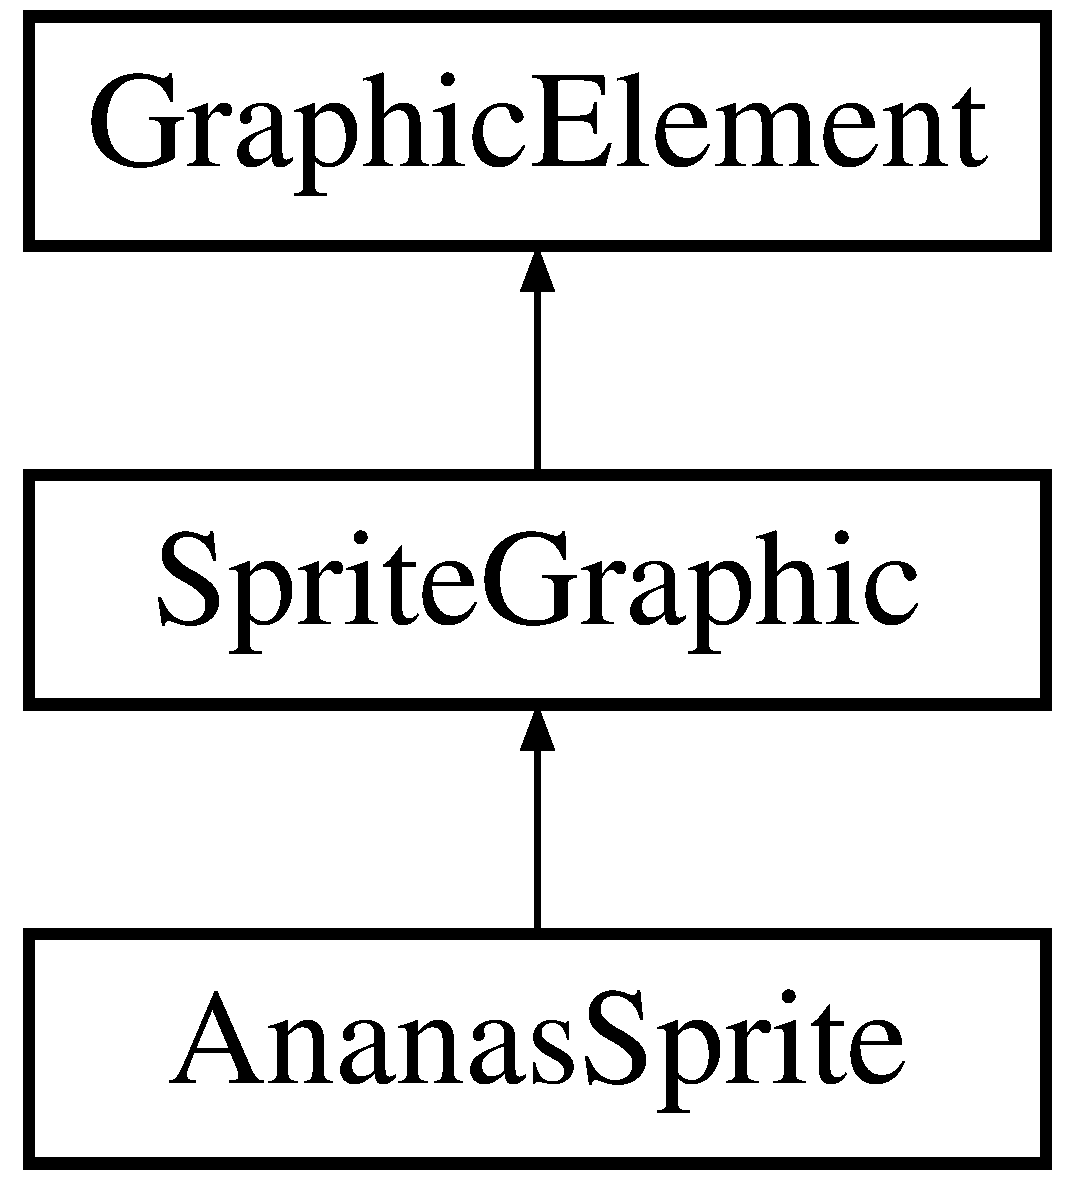
\includegraphics[height=3.000000cm]{class_ananas_sprite}
\end{center}
\end{figure}
\subsection*{Fonctions membres publiques}
\begin{DoxyCompactItemize}
\item 
\hypertarget{class_ananas_sprite_ade2186d7ff94d7d13d4ea771359881d5}{virtual void {\bfseries set\-Image\-To\-Sprite} ()}\label{class_ananas_sprite_ade2186d7ff94d7d13d4ea771359881d5}

\end{DoxyCompactItemize}
\subsection*{Membres hérités additionnels}


La documentation de cette classe a été générée à partir des fichiers suivants \-:\begin{DoxyCompactItemize}
\item 
/\-Users/\-Ananas/\-Desktop/\-Mes\-Projets\-Git/purupurudigger/\-Code\-Cpp/Ananas\-Sprite.\-h\item 
/\-Users/\-Ananas/\-Desktop/\-Mes\-Projets\-Git/purupurudigger/\-Code\-Cpp/Ananas\-Sprite.\-cpp\end{DoxyCompactItemize}

\hypertarget{class_background_graphic}{\section{Référence de la classe Background\-Graphic}
\label{class_background_graphic}\index{Background\-Graphic@{Background\-Graphic}}
}
Graphe d'héritage de Background\-Graphic\-:\begin{figure}[H]
\begin{center}
\leavevmode
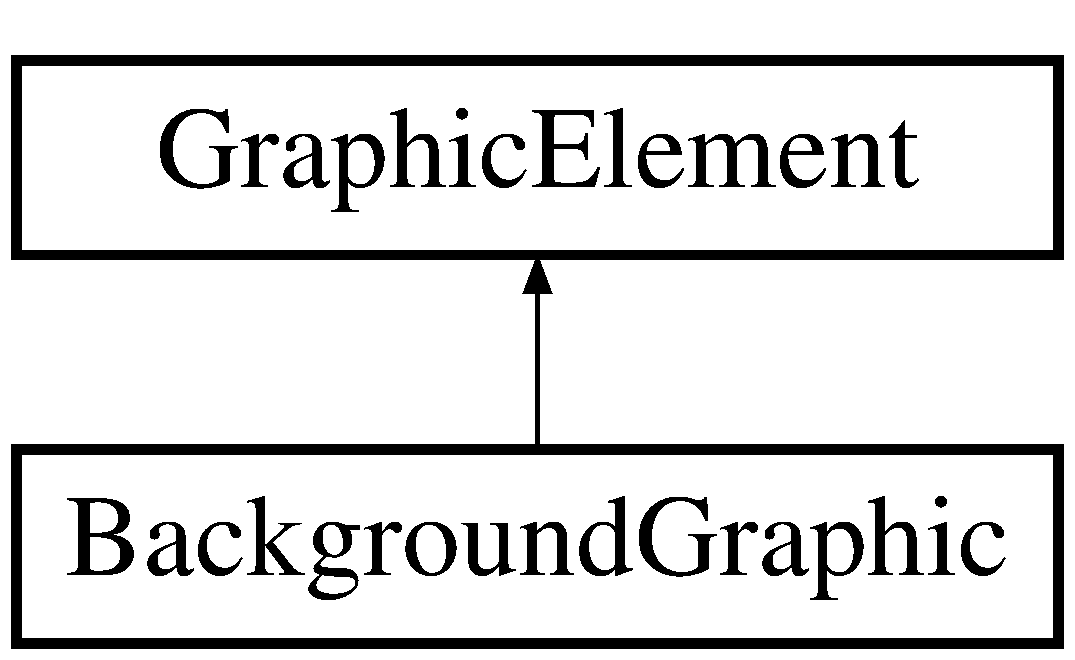
\includegraphics[height=2.000000cm]{class_background_graphic}
\end{center}
\end{figure}
\subsection*{Fonctions membres publiques}
\begin{DoxyCompactItemize}
\item 
\hypertarget{class_background_graphic_a6942ac3404db018c066dd2db1523c8ad}{virtual void {\bfseries set\-Image\-To\-Sprite} ()}\label{class_background_graphic_a6942ac3404db018c066dd2db1523c8ad}

\item 
\hypertarget{class_background_graphic_a4a0302e431b3abd754e49d151f299198}{virtual void {\bfseries set\-Teacher\-Mode} ()}\label{class_background_graphic_a4a0302e431b3abd754e49d151f299198}

\item 
\hypertarget{class_background_graphic_ac7615a6253c7900692addd2619832f8d}{virtual void {\bfseries set\-Ananas\-Mode} ()}\label{class_background_graphic_ac7615a6253c7900692addd2619832f8d}

\end{DoxyCompactItemize}
\subsection*{Attributs protégés statiques}
\begin{DoxyCompactItemize}
\item 
\hypertarget{class_background_graphic_a4aaecbc474b50bd3ea60b4c8b0541074}{static sf\-::\-Image {\bfseries my\-\_\-image}}\label{class_background_graphic_a4aaecbc474b50bd3ea60b4c8b0541074}

\end{DoxyCompactItemize}
\subsection*{Membres hérités additionnels}


La documentation de cette classe a été générée à partir des fichiers suivants \-:\begin{DoxyCompactItemize}
\item 
/\-Users/\-Ananas/\-Desktop/\-Mes\-Projets\-Git/purupurudigger/\-Code\-Cpp/Background\-Graphic.\-h\item 
/\-Users/\-Ananas/\-Desktop/\-Mes\-Projets\-Git/purupurudigger/\-Code\-Cpp/Background\-Graphic.\-cpp\end{DoxyCompactItemize}

\hypertarget{class_bomb}{\section{Référence de la classe Bomb}
\label{class_bomb}\index{Bomb@{Bomb}}
}


Classe modélisant ce qu'est une \hyperlink{class_bomb}{Bomb}.  




{\ttfamily \#include $<$Bomb.\-h$>$}

Graphe d'héritage de Bomb\-:\begin{figure}[H]
\begin{center}
\leavevmode
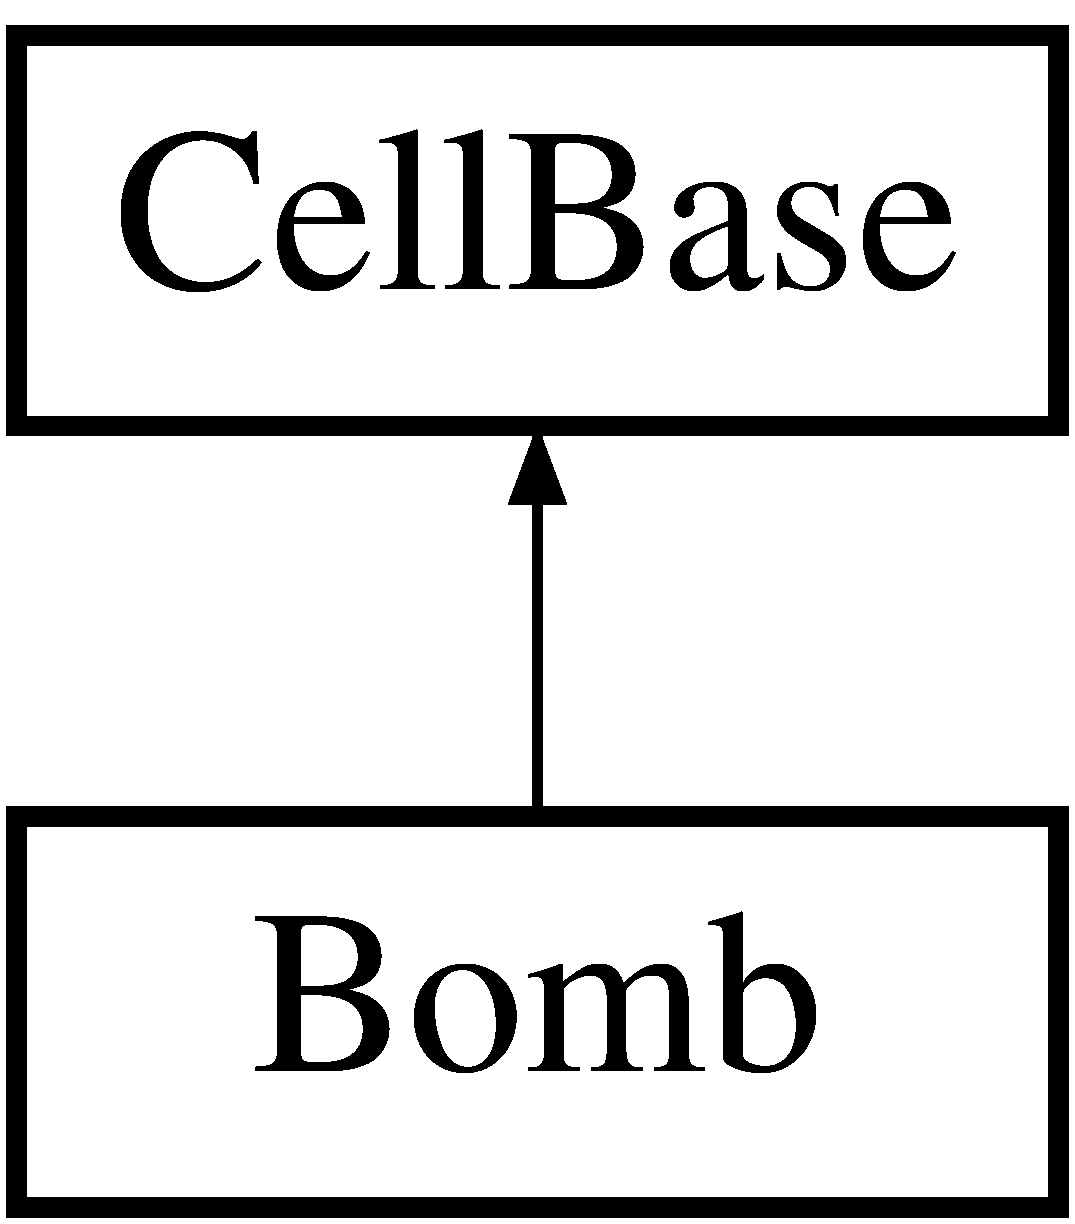
\includegraphics[height=2.000000cm]{class_bomb}
\end{center}
\end{figure}
\subsection*{Fonctions membres publiques}
\begin{DoxyCompactItemize}
\item 
\hyperlink{class_bomb_a5805401b6cfbb451cf31ebd4851740cf}{Bomb} ()
\begin{DoxyCompactList}\small\item\em Constructeur. \end{DoxyCompactList}\item 
\hyperlink{class_bomb_a318b2684bf1c574999874a943478b264}{Bomb} (int x, int y)
\begin{DoxyCompactList}\small\item\em Constructeur paramétré \end{DoxyCompactList}\item 
\hyperlink{class_bomb_a4819197ccba9c9d0e5dc0176baf1e9b2}{Bomb} (const \hyperlink{class_bomb}{Bomb} \&b)
\begin{DoxyCompactList}\small\item\em Constructeur par copie. \end{DoxyCompactList}\item 
virtual \hyperlink{class_bomb_acbb47327cfb2fa429887774ef3597965}{$\sim$\-Bomb} ()
\begin{DoxyCompactList}\small\item\em Destructeur. \end{DoxyCompactList}\item 
virtual \hyperlink{class_bomb}{Bomb} \& \hyperlink{class_bomb_a5b76072fc1f9ee0755823afe65b77db9}{operator=} (const \hyperlink{class_bomb}{Bomb} \&b)
\begin{DoxyCompactList}\small\item\em Opérateur d'affectation pour recopier une case. \end{DoxyCompactList}\end{DoxyCompactItemize}
\subsection*{Membres hérités additionnels}


\subsection{Description détaillée}
Classe modélisant ce qu'est une \hyperlink{class_bomb}{Bomb}. 

\subsection{Documentation des constructeurs et destructeur}
\hypertarget{class_bomb_a5805401b6cfbb451cf31ebd4851740cf}{\index{Bomb@{Bomb}!Bomb@{Bomb}}
\index{Bomb@{Bomb}!Bomb@{Bomb}}
\subsubsection[{Bomb}]{\setlength{\rightskip}{0pt plus 5cm}Bomb\-::\-Bomb (
\begin{DoxyParamCaption}
{}
\end{DoxyParamCaption}
)}}\label{class_bomb_a5805401b6cfbb451cf31ebd4851740cf}


Constructeur. 

Constructeur de la classe \hyperlink{class_bomb}{Bomb} \hypertarget{class_bomb_a318b2684bf1c574999874a943478b264}{\index{Bomb@{Bomb}!Bomb@{Bomb}}
\index{Bomb@{Bomb}!Bomb@{Bomb}}
\subsubsection[{Bomb}]{\setlength{\rightskip}{0pt plus 5cm}Bomb\-::\-Bomb (
\begin{DoxyParamCaption}
\item[{int}]{x, }
\item[{int}]{y}
\end{DoxyParamCaption}
)}}\label{class_bomb_a318b2684bf1c574999874a943478b264}


Constructeur paramétré 

Constructeur paramétré de la classe \hyperlink{class_bomb}{Bomb} \hypertarget{class_bomb_a4819197ccba9c9d0e5dc0176baf1e9b2}{\index{Bomb@{Bomb}!Bomb@{Bomb}}
\index{Bomb@{Bomb}!Bomb@{Bomb}}
\subsubsection[{Bomb}]{\setlength{\rightskip}{0pt plus 5cm}Bomb\-::\-Bomb (
\begin{DoxyParamCaption}
\item[{const {\bf Bomb} \&}]{b}
\end{DoxyParamCaption}
)}}\label{class_bomb_a4819197ccba9c9d0e5dc0176baf1e9b2}


Constructeur par copie. 

Constructeur par copie de la classe \hyperlink{class_bomb}{Bomb} 
\begin{DoxyParams}[1]{Paramètres}
\mbox{\tt in}  & {\em \hyperlink{class_bomb}{Bomb}} & b \\
\hline
\mbox{\tt out}  & {\em \hyperlink{class_bomb}{Bomb}} & b \\
\hline
\end{DoxyParams}
\hypertarget{class_bomb_acbb47327cfb2fa429887774ef3597965}{\index{Bomb@{Bomb}!$\sim$\-Bomb@{$\sim$\-Bomb}}
\index{$\sim$\-Bomb@{$\sim$\-Bomb}!Bomb@{Bomb}}
\subsubsection[{$\sim$\-Bomb}]{\setlength{\rightskip}{0pt plus 5cm}Bomb\-::$\sim$\-Bomb (
\begin{DoxyParamCaption}
{}
\end{DoxyParamCaption}
)\hspace{0.3cm}{\ttfamily [virtual]}}}\label{class_bomb_acbb47327cfb2fa429887774ef3597965}


Destructeur. 

Destructeur de la classe fille \hyperlink{class_bomb}{Bomb} 

\subsection{Documentation des fonctions membres}
\hypertarget{class_bomb_a5b76072fc1f9ee0755823afe65b77db9}{\index{Bomb@{Bomb}!operator=@{operator=}}
\index{operator=@{operator=}!Bomb@{Bomb}}
\subsubsection[{operator=}]{\setlength{\rightskip}{0pt plus 5cm}{\bf Bomb} \& Bomb\-::operator= (
\begin{DoxyParamCaption}
\item[{const {\bf Bomb} \&}]{b}
\end{DoxyParamCaption}
)\hspace{0.3cm}{\ttfamily [virtual]}}}\label{class_bomb_a5b76072fc1f9ee0755823afe65b77db9}


Opérateur d'affectation pour recopier une case. 


\begin{DoxyParams}{Paramètres}
{\em b\mbox{]}} & \hyperlink{class_bomb}{Bomb} c \-: opérateur d'affectation pour recopier une \hyperlink{class_bomb}{Bomb} \\
\hline
\end{DoxyParams}


La documentation de cette classe a été générée à partir des fichiers suivants \-:\begin{DoxyCompactItemize}
\item 
/\-Users/\-Ananas/\-Desktop/\-Mes\-Projets\-Git/purupurudigger/\-Code\-Cpp/\hyperlink{_bomb_8h}{Bomb.\-h}\item 
/\-Users/\-Ananas/\-Desktop/\-Mes\-Projets\-Git/purupurudigger/\-Code\-Cpp/\hyperlink{_bomb_8cpp}{Bomb.\-cpp}\end{DoxyCompactItemize}

\hypertarget{class_bomb_graphic}{\section{Référence de la classe Bomb\-Graphic}
\label{class_bomb_graphic}\index{Bomb\-Graphic@{Bomb\-Graphic}}
}
Graphe d'héritage de Bomb\-Graphic\-:\begin{figure}[H]
\begin{center}
\leavevmode
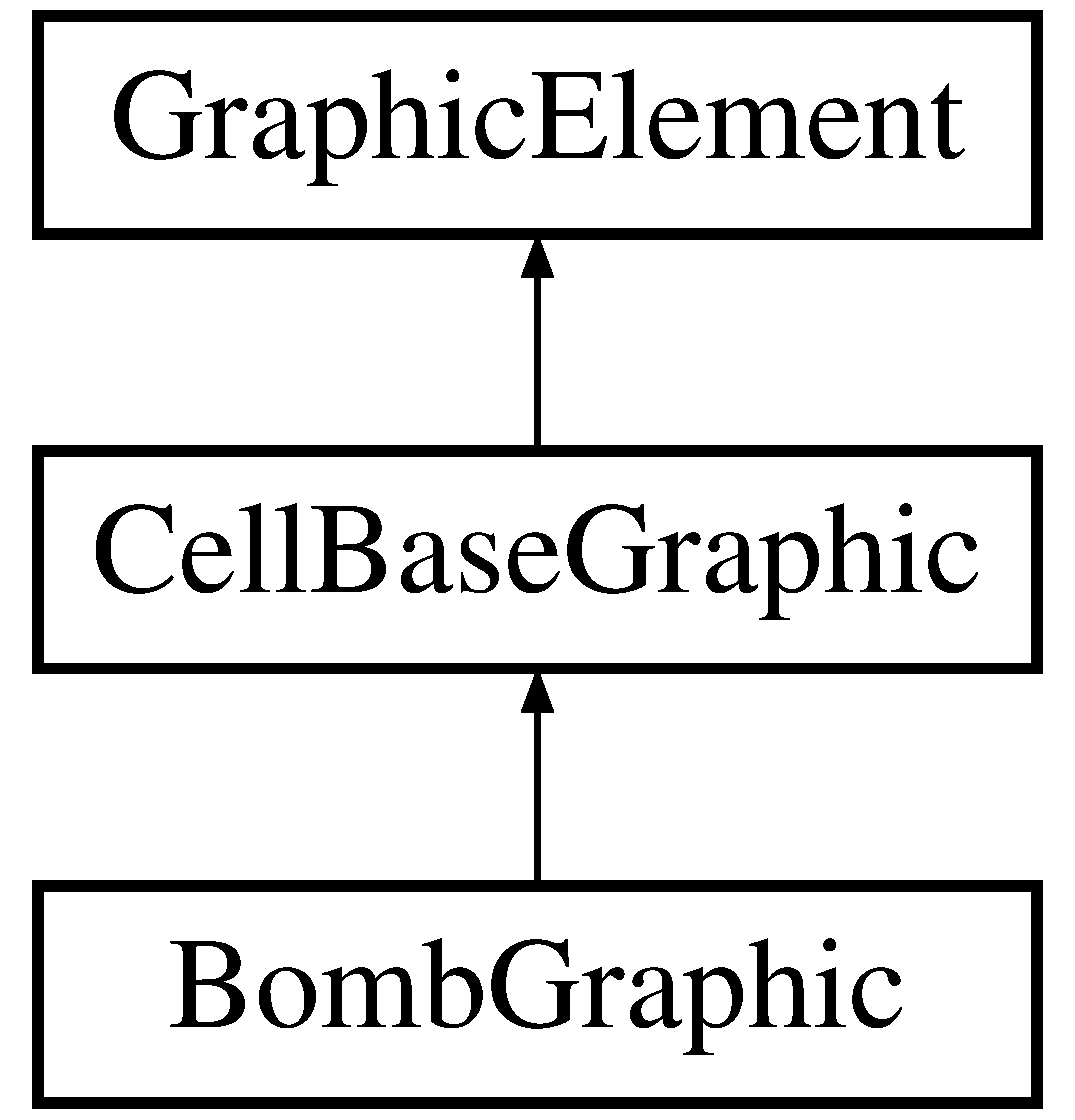
\includegraphics[height=3.000000cm]{class_bomb_graphic}
\end{center}
\end{figure}
\subsection*{Fonctions membres publiques}
\begin{DoxyCompactItemize}
\item 
\hypertarget{class_bomb_graphic_a919767f2decd54bc8f6c75edfad8a3ef}{virtual void {\bfseries set\-Image\-To\-Sprite} ()}\label{class_bomb_graphic_a919767f2decd54bc8f6c75edfad8a3ef}

\end{DoxyCompactItemize}
\subsection*{Membres hérités additionnels}


La documentation de cette classe a été générée à partir des fichiers suivants \-:\begin{DoxyCompactItemize}
\item 
/\-Users/\-Ananas/\-Desktop/\-Mes\-Projets\-Git/purupurudigger/\-Code\-Cpp/Bomb\-Graphic.\-h\item 
/\-Users/\-Ananas/\-Desktop/\-Mes\-Projets\-Git/purupurudigger/\-Code\-Cpp/Bomb\-Graphic.\-cpp\end{DoxyCompactItemize}

\hypertarget{class_button_graphic}{\section{Référence de la classe Button\-Graphic}
\label{class_button_graphic}\index{Button\-Graphic@{Button\-Graphic}}
}
Graphe d'héritage de Button\-Graphic\-:\begin{figure}[H]
\begin{center}
\leavevmode
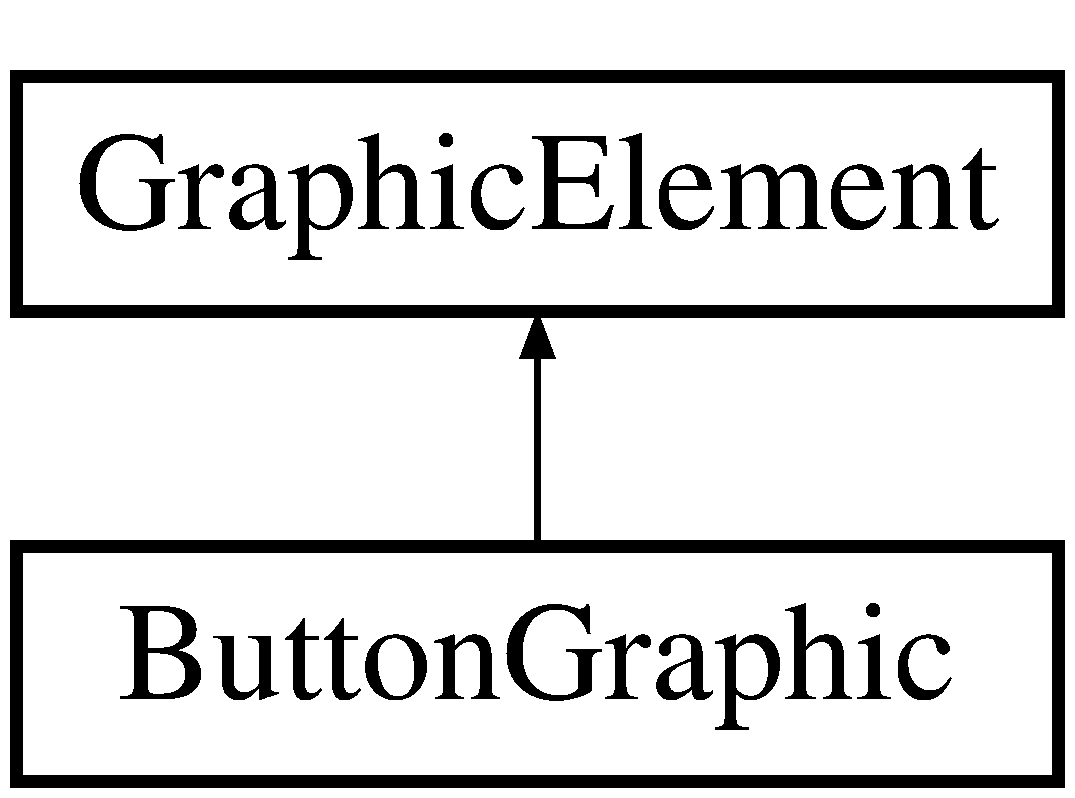
\includegraphics[height=2.000000cm]{class_button_graphic}
\end{center}
\end{figure}
\subsection*{Fonctions membres publiques}
\begin{DoxyCompactItemize}
\item 
\hypertarget{class_button_graphic_a4d34450a0f45dfc3569e3519de72eced}{virtual void {\bfseries set\-Image\-To\-Sprite} ()}\label{class_button_graphic_a4d34450a0f45dfc3569e3519de72eced}

\item 
\hypertarget{class_button_graphic_a2aaf45618764fd342fe39646d24a2c75}{virtual void {\bfseries set\-Teacher\-Mode} ()}\label{class_button_graphic_a2aaf45618764fd342fe39646d24a2c75}

\item 
\hypertarget{class_button_graphic_a087503d732dded5b8006c48c9047b736}{virtual void {\bfseries set\-Ananas\-Mode} ()}\label{class_button_graphic_a087503d732dded5b8006c48c9047b736}

\item 
\hypertarget{class_button_graphic_a8e406b9618765edc7b1f9ee7568c0def}{virtual void {\bfseries set\-Sprite\-And\-Draw} (int x, int y, sf\-::\-Render\-Window $\ast$\-\_\-window, std\-::string)}\label{class_button_graphic_a8e406b9618765edc7b1f9ee7568c0def}

\item 
\hypertarget{class_button_graphic_a2fed2c1bf6dc330998497efbf4347b87}{void {\bfseries set\-Hover} ()}\label{class_button_graphic_a2fed2c1bf6dc330998497efbf4347b87}

\item 
\hypertarget{class_button_graphic_a85728fbd0bad0617622398c1328037fc}{void {\bfseries reset} ()}\label{class_button_graphic_a85728fbd0bad0617622398c1328037fc}

\item 
\hypertarget{class_button_graphic_a19b792938f2ee0b681a8f73d3119e726}{virtual void {\bfseries draw} (sf\-::\-Render\-Window $\ast$\-\_\-window) const }\label{class_button_graphic_a19b792938f2ee0b681a8f73d3119e726}

\end{DoxyCompactItemize}
\subsection*{Attributs protégés}
\begin{DoxyCompactItemize}
\item 
\hypertarget{class_button_graphic_a5c0fc023a5c6856ca1f87a5a7601f24c}{sf\-::\-String {\bfseries my\-\_\-string}}\label{class_button_graphic_a5c0fc023a5c6856ca1f87a5a7601f24c}

\end{DoxyCompactItemize}
\subsection*{Attributs protégés statiques}
\begin{DoxyCompactItemize}
\item 
\hypertarget{class_button_graphic_a6ebb6c74733ac73702df072afbb684fc}{static sf\-::\-Image {\bfseries my\-\_\-image}}\label{class_button_graphic_a6ebb6c74733ac73702df072afbb684fc}

\item 
\hypertarget{class_button_graphic_aebc358786eeb35bf58959c62fc1bfa27}{static sf\-::\-Font {\bfseries my\-\_\-font}}\label{class_button_graphic_aebc358786eeb35bf58959c62fc1bfa27}

\end{DoxyCompactItemize}


La documentation de cette classe a été générée à partir des fichiers suivants \-:\begin{DoxyCompactItemize}
\item 
/\-Users/\-Ananas/\-Desktop/\-Mes\-Projets\-Git/purupurudigger/\-Code\-Cpp/Button\-Graphic.\-h\item 
/\-Users/\-Ananas/\-Desktop/\-Mes\-Projets\-Git/purupurudigger/\-Code\-Cpp/Button\-Graphic.\-cpp\end{DoxyCompactItemize}

\hypertarget{class_cell_base}{\section{Référence de la classe Cell\-Base}
\label{class_cell_base}\index{Cell\-Base@{Cell\-Base}}
}


Classe modélisant ce qu'est une case.  




{\ttfamily \#include $<$Cell\-Base.\-h$>$}

Graphe d'héritage de Cell\-Base\-:\begin{figure}[H]
\begin{center}
\leavevmode
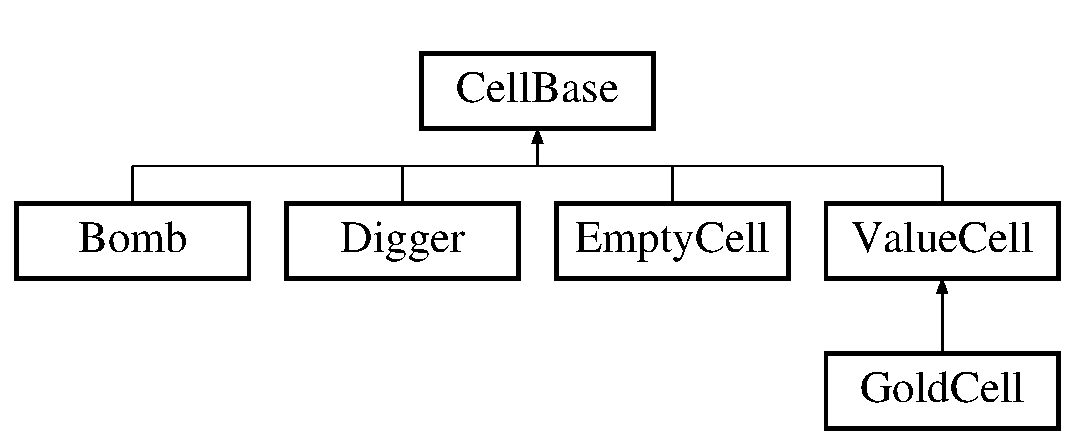
\includegraphics[height=3.000000cm]{class_cell_base}
\end{center}
\end{figure}
\subsection*{Fonctions membres publiques}
\begin{DoxyCompactItemize}
\item 
\hyperlink{class_cell_base_ac5cbc18d3f767bb91d9e052a3eb778b5}{Cell\-Base} ()
\begin{DoxyCompactList}\small\item\em Constructeur. \end{DoxyCompactList}\item 
\hyperlink{class_cell_base_a12169f30ca7038d58bdf810cb6314df0}{Cell\-Base} (int x, int y)
\begin{DoxyCompactList}\small\item\em Constructeur paramétré \end{DoxyCompactList}\item 
\hyperlink{class_cell_base_ae2b545b0d403816ba1d572cee7f97ec9}{Cell\-Base} (const \hyperlink{class_cell_base}{Cell\-Base} \&c)
\begin{DoxyCompactList}\small\item\em Constructeur par copie. \end{DoxyCompactList}\item 
virtual \hyperlink{class_cell_base_a91df7ce6090723939914fc08ae5dd25e}{$\sim$\-Cell\-Base} ()
\begin{DoxyCompactList}\small\item\em Destructeur. \end{DoxyCompactList}\item 
int \hyperlink{class_cell_base_a0df4af1a9faa0e1bc1d2ac22947b3281}{get\-X} () const 
\begin{DoxyCompactList}\small\item\em retourne la position en X de la case \end{DoxyCompactList}\item 
int \hyperlink{class_cell_base_a51f37b58bdf1ef4d51d956d02f35b411}{get\-Y} () const 
\begin{DoxyCompactList}\small\item\em retourne la position en Y de la case \end{DoxyCompactList}\item 
void \hyperlink{class_cell_base_a3280e04207e4419d425913d519fb867d}{set\-X} (int x)
\begin{DoxyCompactList}\small\item\em Pour positionner notre case dans la grille. \end{DoxyCompactList}\item 
void \hyperlink{class_cell_base_a5c2f67f6bb1ba06b42c90d81b5ed872a}{set\-Y} (int y)
\begin{DoxyCompactList}\small\item\em Pour positionner notre case dans la grille. \end{DoxyCompactList}\item 
virtual \hyperlink{class_cell_base}{Cell\-Base} \& \hyperlink{class_cell_base_a31f5f4bcdc5e254476b376eadc8fa2f6}{operator=} (const \hyperlink{class_cell_base}{Cell\-Base} \&c)
\begin{DoxyCompactList}\small\item\em Opérateur d'affectation pour recopier une case. \end{DoxyCompactList}\item 
\hypertarget{class_cell_base_aae6d1d9ee7ad46d21c4ac6e698cd2754}{std\-::string {\bfseries get\-Type} ()}\label{class_cell_base_aae6d1d9ee7ad46d21c4ac6e698cd2754}

\end{DoxyCompactItemize}
\subsection*{Fonctions membres protégées}
\begin{DoxyCompactItemize}
\item 
\hypertarget{class_cell_base_a1f9036ed8d703f7b341b49eec4fd8882}{virtual void {\bfseries to\-Clone} (const \hyperlink{class_cell_base}{Cell\-Base} \&c)}\label{class_cell_base_a1f9036ed8d703f7b341b49eec4fd8882}

\end{DoxyCompactItemize}
\subsection*{Attributs protégés}
\begin{DoxyCompactItemize}
\item 
std\-::string \hyperlink{class_cell_base_a4039c6141e348f927d90297d01e19509}{my\-\_\-type}
\item 
int \hyperlink{class_cell_base_a9dc2714aa92817ba6a6a23da19eb4fde}{my\-\_\-x}
\item 
int \hyperlink{class_cell_base_a39722b0f229e34f50c7b9d4d12d19a52}{my\-\_\-y}
\end{DoxyCompactItemize}


\subsection{Description détaillée}
Classe modélisant ce qu'est une case. 

\subsection{Documentation des constructeurs et destructeur}
\hypertarget{class_cell_base_ac5cbc18d3f767bb91d9e052a3eb778b5}{\index{Cell\-Base@{Cell\-Base}!Cell\-Base@{Cell\-Base}}
\index{Cell\-Base@{Cell\-Base}!CellBase@{Cell\-Base}}
\subsubsection[{Cell\-Base}]{\setlength{\rightskip}{0pt plus 5cm}Cell\-Base\-::\-Cell\-Base (
\begin{DoxyParamCaption}
{}
\end{DoxyParamCaption}
)}}\label{class_cell_base_ac5cbc18d3f767bb91d9e052a3eb778b5}


Constructeur. 

Constructeur de la classe \hyperlink{class_cell_base}{Cell\-Base} \hypertarget{class_cell_base_a12169f30ca7038d58bdf810cb6314df0}{\index{Cell\-Base@{Cell\-Base}!Cell\-Base@{Cell\-Base}}
\index{Cell\-Base@{Cell\-Base}!CellBase@{Cell\-Base}}
\subsubsection[{Cell\-Base}]{\setlength{\rightskip}{0pt plus 5cm}Cell\-Base\-::\-Cell\-Base (
\begin{DoxyParamCaption}
\item[{int}]{x, }
\item[{int}]{y}
\end{DoxyParamCaption}
)}}\label{class_cell_base_a12169f30ca7038d58bdf810cb6314df0}


Constructeur paramétré 

Constructeur paramétré de la classe \hyperlink{class_cell_base}{Cell\-Base} \hypertarget{class_cell_base_ae2b545b0d403816ba1d572cee7f97ec9}{\index{Cell\-Base@{Cell\-Base}!Cell\-Base@{Cell\-Base}}
\index{Cell\-Base@{Cell\-Base}!CellBase@{Cell\-Base}}
\subsubsection[{Cell\-Base}]{\setlength{\rightskip}{0pt plus 5cm}Cell\-Base\-::\-Cell\-Base (
\begin{DoxyParamCaption}
\item[{const {\bf Cell\-Base} \&}]{c}
\end{DoxyParamCaption}
)}}\label{class_cell_base_ae2b545b0d403816ba1d572cee7f97ec9}


Constructeur par copie. 

Constructeur par copie de la classe \hyperlink{class_cell_base}{Cell\-Base} \hypertarget{class_cell_base_a91df7ce6090723939914fc08ae5dd25e}{\index{Cell\-Base@{Cell\-Base}!$\sim$\-Cell\-Base@{$\sim$\-Cell\-Base}}
\index{$\sim$\-Cell\-Base@{$\sim$\-Cell\-Base}!CellBase@{Cell\-Base}}
\subsubsection[{$\sim$\-Cell\-Base}]{\setlength{\rightskip}{0pt plus 5cm}Cell\-Base\-::$\sim$\-Cell\-Base (
\begin{DoxyParamCaption}
{}
\end{DoxyParamCaption}
)\hspace{0.3cm}{\ttfamily [virtual]}}}\label{class_cell_base_a91df7ce6090723939914fc08ae5dd25e}


Destructeur. 

Destructeur de la classe mère \hyperlink{class_cell_base}{Cell\-Base} 

\subsection{Documentation des fonctions membres}
\hypertarget{class_cell_base_a0df4af1a9faa0e1bc1d2ac22947b3281}{\index{Cell\-Base@{Cell\-Base}!get\-X@{get\-X}}
\index{get\-X@{get\-X}!CellBase@{Cell\-Base}}
\subsubsection[{get\-X}]{\setlength{\rightskip}{0pt plus 5cm}int Cell\-Base\-::get\-X (
\begin{DoxyParamCaption}
{}
\end{DoxyParamCaption}
) const}}\label{class_cell_base_a0df4af1a9faa0e1bc1d2ac22947b3281}


retourne la position en X de la case 

\begin{DoxyReturn}{Renvoie}
l'entier positionnant notre case en X 
\end{DoxyReturn}
\hypertarget{class_cell_base_a51f37b58bdf1ef4d51d956d02f35b411}{\index{Cell\-Base@{Cell\-Base}!get\-Y@{get\-Y}}
\index{get\-Y@{get\-Y}!CellBase@{Cell\-Base}}
\subsubsection[{get\-Y}]{\setlength{\rightskip}{0pt plus 5cm}int Cell\-Base\-::get\-Y (
\begin{DoxyParamCaption}
{}
\end{DoxyParamCaption}
) const}}\label{class_cell_base_a51f37b58bdf1ef4d51d956d02f35b411}


retourne la position en Y de la case 

\begin{DoxyReturn}{Renvoie}
l'entier positionnant notre case en Y 
\end{DoxyReturn}
\hypertarget{class_cell_base_a31f5f4bcdc5e254476b376eadc8fa2f6}{\index{Cell\-Base@{Cell\-Base}!operator=@{operator=}}
\index{operator=@{operator=}!CellBase@{Cell\-Base}}
\subsubsection[{operator=}]{\setlength{\rightskip}{0pt plus 5cm}{\bf Cell\-Base} \& Cell\-Base\-::operator= (
\begin{DoxyParamCaption}
\item[{const {\bf Cell\-Base} \&}]{c}
\end{DoxyParamCaption}
)\hspace{0.3cm}{\ttfamily [virtual]}}}\label{class_cell_base_a31f5f4bcdc5e254476b376eadc8fa2f6}


Opérateur d'affectation pour recopier une case. 

param\mbox{[}c\mbox{]} \hyperlink{class_cell_base}{Cell\-Base} c \-: opérateur d'affectation pour recopier une case \hypertarget{class_cell_base_a3280e04207e4419d425913d519fb867d}{\index{Cell\-Base@{Cell\-Base}!set\-X@{set\-X}}
\index{set\-X@{set\-X}!CellBase@{Cell\-Base}}
\subsubsection[{set\-X}]{\setlength{\rightskip}{0pt plus 5cm}void Cell\-Base\-::set\-X (
\begin{DoxyParamCaption}
\item[{int}]{x}
\end{DoxyParamCaption}
)}}\label{class_cell_base_a3280e04207e4419d425913d519fb867d}


Pour positionner notre case dans la grille. 

param\mbox{[}in\mbox{]} int x \-: la position verticale de notre case \hypertarget{class_cell_base_a5c2f67f6bb1ba06b42c90d81b5ed872a}{\index{Cell\-Base@{Cell\-Base}!set\-Y@{set\-Y}}
\index{set\-Y@{set\-Y}!CellBase@{Cell\-Base}}
\subsubsection[{set\-Y}]{\setlength{\rightskip}{0pt plus 5cm}void Cell\-Base\-::set\-Y (
\begin{DoxyParamCaption}
\item[{int}]{y}
\end{DoxyParamCaption}
)}}\label{class_cell_base_a5c2f67f6bb1ba06b42c90d81b5ed872a}


Pour positionner notre case dans la grille. 

param\mbox{[}in\mbox{]} int x \-: la position horizontale de notre case 

\subsection{Documentation des données membres}
\hypertarget{class_cell_base_a4039c6141e348f927d90297d01e19509}{\index{Cell\-Base@{Cell\-Base}!my\-\_\-type@{my\-\_\-type}}
\index{my\-\_\-type@{my\-\_\-type}!CellBase@{Cell\-Base}}
\subsubsection[{my\-\_\-type}]{\setlength{\rightskip}{0pt plus 5cm}std\-::string Cell\-Base\-::my\-\_\-type\hspace{0.3cm}{\ttfamily [protected]}}}\label{class_cell_base_a4039c6141e348f927d90297d01e19509}
le type de ma case \hypertarget{class_cell_base_a9dc2714aa92817ba6a6a23da19eb4fde}{\index{Cell\-Base@{Cell\-Base}!my\-\_\-x@{my\-\_\-x}}
\index{my\-\_\-x@{my\-\_\-x}!CellBase@{Cell\-Base}}
\subsubsection[{my\-\_\-x}]{\setlength{\rightskip}{0pt plus 5cm}int Cell\-Base\-::my\-\_\-x\hspace{0.3cm}{\ttfamily [protected]}}}\label{class_cell_base_a9dc2714aa92817ba6a6a23da19eb4fde}
Le x de ma case \hypertarget{class_cell_base_a39722b0f229e34f50c7b9d4d12d19a52}{\index{Cell\-Base@{Cell\-Base}!my\-\_\-y@{my\-\_\-y}}
\index{my\-\_\-y@{my\-\_\-y}!CellBase@{Cell\-Base}}
\subsubsection[{my\-\_\-y}]{\setlength{\rightskip}{0pt plus 5cm}int Cell\-Base\-::my\-\_\-y\hspace{0.3cm}{\ttfamily [protected]}}}\label{class_cell_base_a39722b0f229e34f50c7b9d4d12d19a52}
Le y de ma case 

La documentation de cette classe a été générée à partir des fichiers suivants \-:\begin{DoxyCompactItemize}
\item 
/\-Users/\-Ananas/\-Desktop/\-Mes\-Projets\-Git/purupurudigger/\-Code\-Cpp/\hyperlink{_cell_base_8h}{Cell\-Base.\-h}\item 
/\-Users/\-Ananas/\-Desktop/\-Mes\-Projets\-Git/purupurudigger/\-Code\-Cpp/\hyperlink{_cell_base_8cpp}{Cell\-Base.\-cpp}\end{DoxyCompactItemize}

\hypertarget{class_cell_base_graphic}{\section{Référence de la classe Cell\-Base\-Graphic}
\label{class_cell_base_graphic}\index{Cell\-Base\-Graphic@{Cell\-Base\-Graphic}}
}
Graphe d'héritage de Cell\-Base\-Graphic\-:\begin{figure}[H]
\begin{center}
\leavevmode
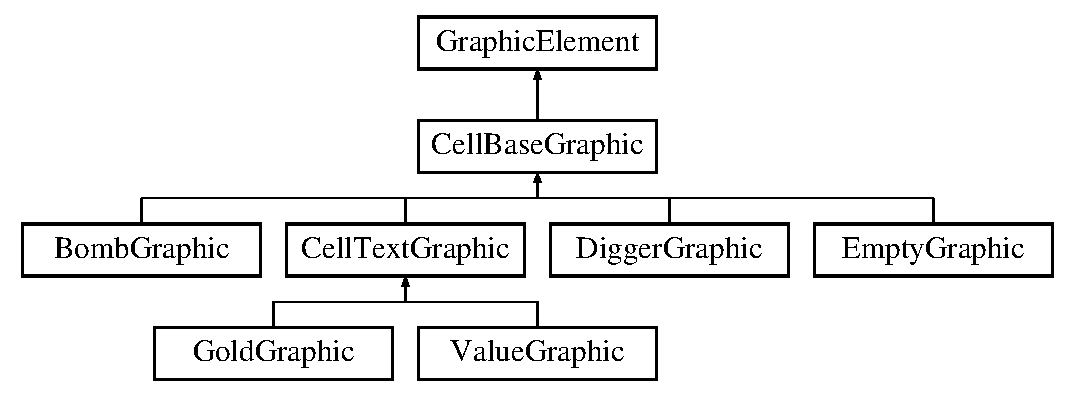
\includegraphics[height=4.000000cm]{class_cell_base_graphic}
\end{center}
\end{figure}
\subsection*{Fonctions membres publiques}
\begin{DoxyCompactItemize}
\item 
\hypertarget{class_cell_base_graphic_a8098385db84f6db111d2f3223f3d4a06}{void {\bfseries set\-Ananas\-Mode} ()}\label{class_cell_base_graphic_a8098385db84f6db111d2f3223f3d4a06}

\item 
\hypertarget{class_cell_base_graphic_a42d524a8413fcdd6af45a255b2a729f6}{void {\bfseries set\-Teacher\-Mode} ()}\label{class_cell_base_graphic_a42d524a8413fcdd6af45a255b2a729f6}

\item 
\hypertarget{class_cell_base_graphic_a4cb2ea2e3e7543a6c71ad1c189f980fe}{virtual void {\bfseries set\-Image\-To\-Sprite} ()}\label{class_cell_base_graphic_a4cb2ea2e3e7543a6c71ad1c189f980fe}

\end{DoxyCompactItemize}
\subsection*{Attributs protégés statiques}
\begin{DoxyCompactItemize}
\item 
\hypertarget{class_cell_base_graphic_a2005f0c436ef5192da542cb2d4bd1f4c}{static sf\-::\-Image {\bfseries my\-\_\-image}}\label{class_cell_base_graphic_a2005f0c436ef5192da542cb2d4bd1f4c}

\end{DoxyCompactItemize}
\subsection*{Membres hérités additionnels}


La documentation de cette classe a été générée à partir des fichiers suivants \-:\begin{DoxyCompactItemize}
\item 
/\-Users/\-Ananas/\-Desktop/\-Mes\-Projets\-Git/purupurudigger/\-Code\-Cpp/Cell\-Base\-Graphic.\-h\item 
/\-Users/\-Ananas/\-Desktop/\-Mes\-Projets\-Git/purupurudigger/\-Code\-Cpp/Cell\-Base\-Graphic.\-cpp\end{DoxyCompactItemize}

\hypertarget{class_cell_text_graphic}{\section{Référence de la classe Cell\-Text\-Graphic}
\label{class_cell_text_graphic}\index{Cell\-Text\-Graphic@{Cell\-Text\-Graphic}}
}
Graphe d'héritage de Cell\-Text\-Graphic\-:\begin{figure}[H]
\begin{center}
\leavevmode
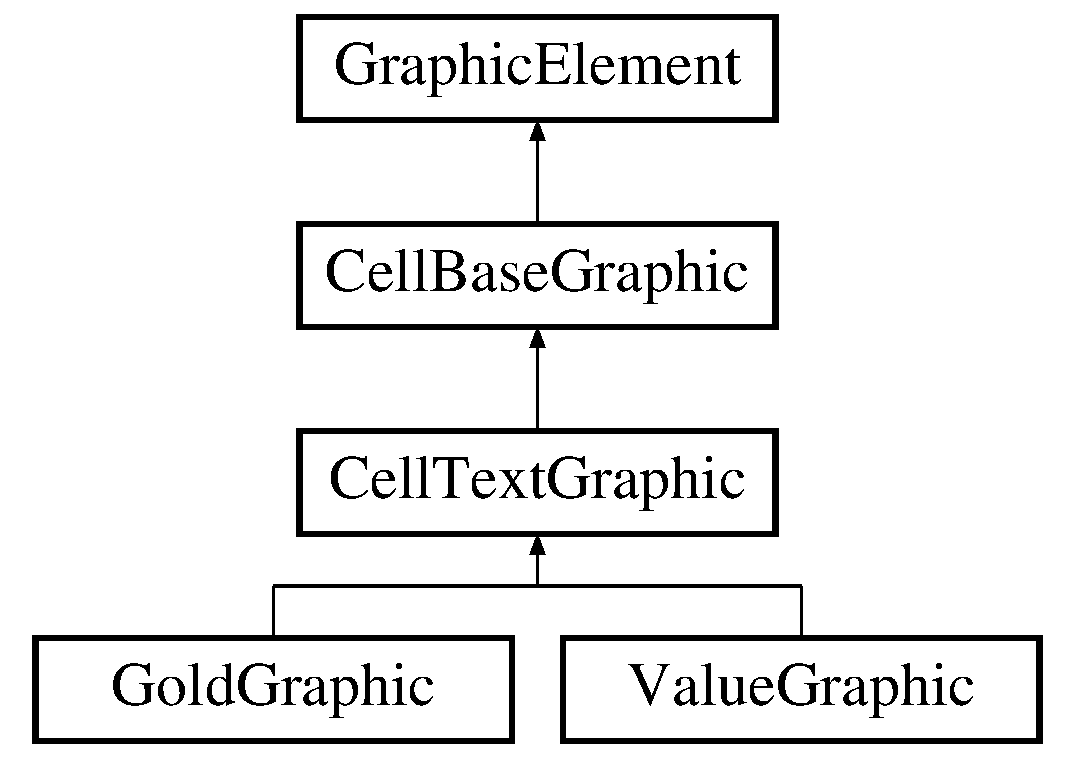
\includegraphics[height=4.000000cm]{class_cell_text_graphic}
\end{center}
\end{figure}
\subsection*{Fonctions membres publiques}
\begin{DoxyCompactItemize}
\item 
\hypertarget{class_cell_text_graphic_adc86a0a31ed4d6c4d50f5b0267008d2f}{virtual void {\bfseries set\-Ananas\-Mode} ()}\label{class_cell_text_graphic_adc86a0a31ed4d6c4d50f5b0267008d2f}

\item 
\hypertarget{class_cell_text_graphic_a8cf1549a23ffa44543819ef3b11e3fad}{virtual void {\bfseries set\-Teacher\-Mode} ()}\label{class_cell_text_graphic_a8cf1549a23ffa44543819ef3b11e3fad}

\item 
\hypertarget{class_cell_text_graphic_ad5f099b24da5923dcdf86274466c2630}{virtual void {\bfseries set\-Sprite\-And\-Draw} (int x, int y, sf\-::\-Render\-Window $\ast$\-\_\-window, std\-::string \-\_\-string)}\label{class_cell_text_graphic_ad5f099b24da5923dcdf86274466c2630}

\item 
\hypertarget{class_cell_text_graphic_a7d8d3ec20aa796b6ae882291b043f0f8}{virtual void {\bfseries set\-Image\-To\-Sprite} ()}\label{class_cell_text_graphic_a7d8d3ec20aa796b6ae882291b043f0f8}

\end{DoxyCompactItemize}
\subsection*{Attributs protégés}
\begin{DoxyCompactItemize}
\item 
\hypertarget{class_cell_text_graphic_ad701261feb308e2da626479a5f746515}{sf\-::\-String {\bfseries my\-\_\-string}}\label{class_cell_text_graphic_ad701261feb308e2da626479a5f746515}

\end{DoxyCompactItemize}
\subsection*{Attributs protégés statiques}
\begin{DoxyCompactItemize}
\item 
\hypertarget{class_cell_text_graphic_aa2ec7dc0bd72bbc7329cee2f17303405}{static sf\-::\-Font {\bfseries my\-\_\-font}}\label{class_cell_text_graphic_aa2ec7dc0bd72bbc7329cee2f17303405}

\end{DoxyCompactItemize}


La documentation de cette classe a été générée à partir des fichiers suivants \-:\begin{DoxyCompactItemize}
\item 
/\-Users/\-Ananas/\-Desktop/\-Mes\-Projets\-Git/purupurudigger/\-Code\-Cpp/Cell\-Text\-Graphic.\-h\item 
/\-Users/\-Ananas/\-Desktop/\-Mes\-Projets\-Git/purupurudigger/\-Code\-Cpp/Cell\-Text\-Graphic.\-cpp\end{DoxyCompactItemize}

\hypertarget{class_dec_functor}{\section{Référence de la classe Dec\-Functor}
\label{class_dec_functor}\index{Dec\-Functor@{Dec\-Functor}}
}


Foncteur pour trier une map à l'envers.  




{\ttfamily \#include $<$Int\-Dec\-Functor.\-h$>$}

\subsection*{Fonctions membres publiques}
\begin{DoxyCompactItemize}
\item 
{\footnotesize template$<$typename T , typename S $>$ }\\bool \hyperlink{class_dec_functor_aa76938dc740d51f98cda440e01946dc5}{operator()} (T n1, S n2)
\begin{DoxyCompactList}\small\item\em Constructeur. \end{DoxyCompactList}\end{DoxyCompactItemize}


\subsection{Description détaillée}
Foncteur pour trier une map à l'envers. 

\subsection{Documentation des fonctions membres}
\hypertarget{class_dec_functor_aa76938dc740d51f98cda440e01946dc5}{\index{Dec\-Functor@{Dec\-Functor}!operator()@{operator()}}
\index{operator()@{operator()}!DecFunctor@{Dec\-Functor}}
\subsubsection[{operator()}]{\setlength{\rightskip}{0pt plus 5cm}template$<$typename T , typename S $>$ bool Dec\-Functor\-::operator() (
\begin{DoxyParamCaption}
\item[{T}]{n1, }
\item[{S}]{n2}
\end{DoxyParamCaption}
)\hspace{0.3cm}{\ttfamily [inline]}}}\label{class_dec_functor_aa76938dc740d51f98cda440e01946dc5}


Constructeur. 

$<$ Notre template


\begin{DoxyParams}[1]{Paramètres}
\mbox{\tt in}  & {\em T} & n1 \\
\hline
\mbox{\tt in}  & {\em S} & n2 \\
\hline
\end{DoxyParams}
\begin{DoxyReturn}{Renvoie}
booléen pour le sens 
\end{DoxyReturn}


La documentation de cette classe a été générée à partir du fichier suivant \-:\begin{DoxyCompactItemize}
\item 
/\-Users/\-Ananas/\-Desktop/\-Mes\-Projets\-Git/purupurudigger/\-Code\-Cpp/\hyperlink{_int_dec_functor_8h}{Int\-Dec\-Functor.\-h}\end{DoxyCompactItemize}

\hypertarget{class_deutsch_graphic}{\section{Référence de la classe Deutsch\-Graphic}
\label{class_deutsch_graphic}\index{Deutsch\-Graphic@{Deutsch\-Graphic}}
}
Graphe d'héritage de Deutsch\-Graphic\-:\begin{figure}[H]
\begin{center}
\leavevmode
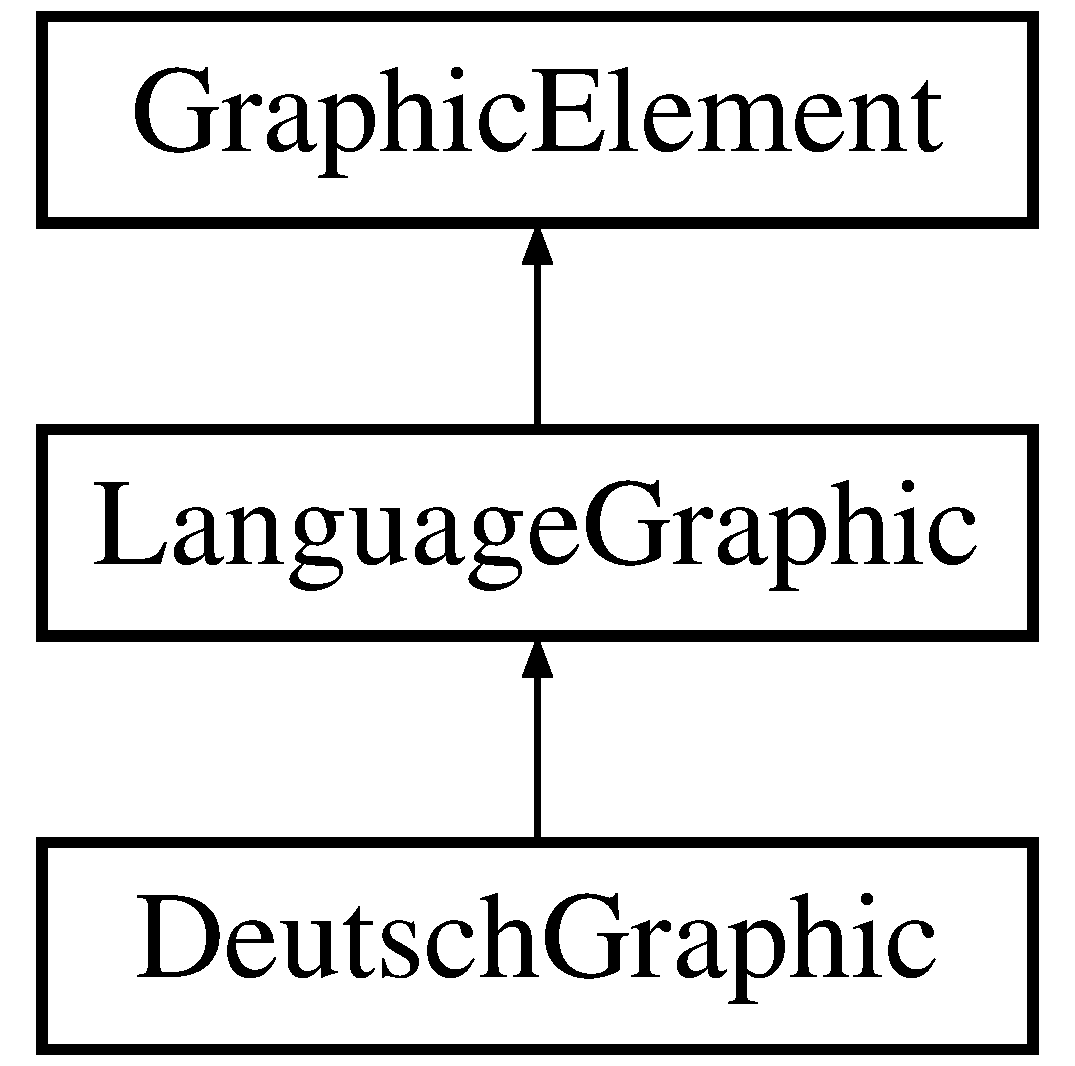
\includegraphics[height=3.000000cm]{class_deutsch_graphic}
\end{center}
\end{figure}
\subsection*{Fonctions membres publiques}
\begin{DoxyCompactItemize}
\item 
\hypertarget{class_deutsch_graphic_a8fb829b3ab050c52fe3a4cdbafc152f0}{virtual void {\bfseries set\-Image\-To\-Sprite} ()}\label{class_deutsch_graphic_a8fb829b3ab050c52fe3a4cdbafc152f0}

\end{DoxyCompactItemize}
\subsection*{Membres hérités additionnels}


La documentation de cette classe a été générée à partir des fichiers suivants \-:\begin{DoxyCompactItemize}
\item 
/\-Users/\-Ananas/\-Desktop/\-Mes\-Projets\-Git/purupurudigger/\-Code\-Cpp/Deutsch\-Graphic.\-h\item 
/\-Users/\-Ananas/\-Desktop/\-Mes\-Projets\-Git/purupurudigger/\-Code\-Cpp/Deutsch\-Graphic.\-cpp\end{DoxyCompactItemize}

\hypertarget{class_digger}{\section{Référence de la classe Digger}
\label{class_digger}\index{Digger@{Digger}}
}


Classe modélisant ce qu'est un digger.  




{\ttfamily \#include $<$Digger.\-h$>$}

Graphe d'héritage de Digger\-:\begin{figure}[H]
\begin{center}
\leavevmode
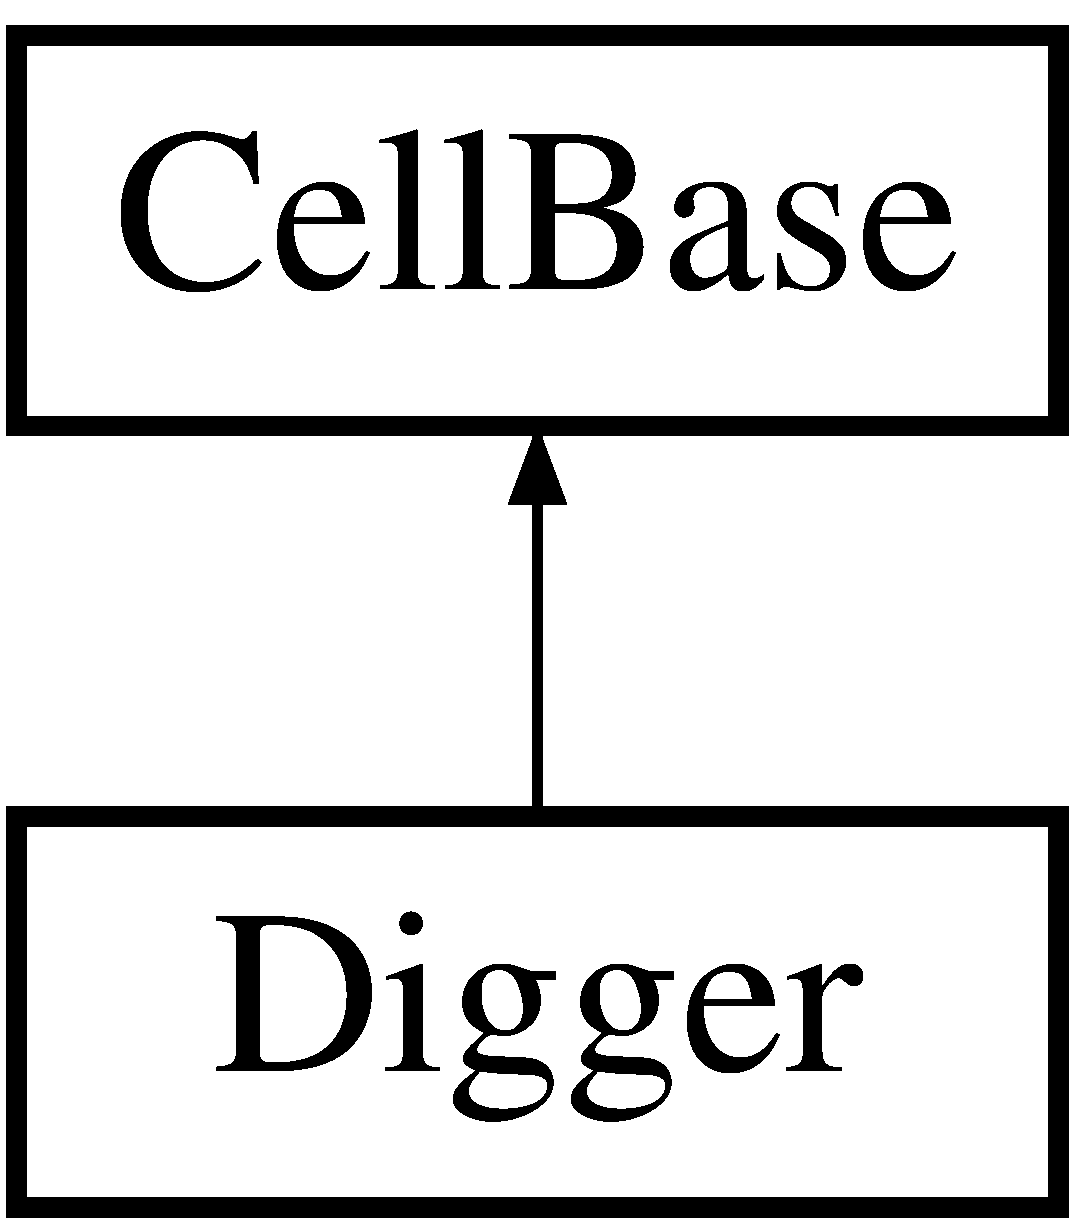
\includegraphics[height=2.000000cm]{class_digger}
\end{center}
\end{figure}
\subsection*{Fonctions membres publiques}
\begin{DoxyCompactItemize}
\item 
\hyperlink{class_digger_ab712cca1629d630478971e1ebeae14ed}{Digger} ()
\begin{DoxyCompactList}\small\item\em Constructeur. \end{DoxyCompactList}\item 
\hyperlink{class_digger_abf3aff066cf3adacd0c449eb7e420e69}{Digger} (int x, int y)
\begin{DoxyCompactList}\small\item\em Constructeur paramétré \end{DoxyCompactList}\item 
\hyperlink{class_digger_a393843f6e9a11b36bb37fba78d5103e2}{Digger} (const \hyperlink{class_digger}{Digger} \&d)
\begin{DoxyCompactList}\small\item\em Constructeur par copie. \end{DoxyCompactList}\item 
virtual \hyperlink{class_digger_a5660a95d7f3d1bfe5c8a754b12e52652}{$\sim$\-Digger} ()
\begin{DoxyCompactList}\small\item\em Destructeur. \end{DoxyCompactList}\item 
int \hyperlink{class_digger_aa6ddf774365ef0913ad360fe23bd715f}{get\-Life} () const 
\begin{DoxyCompactList}\small\item\em Retourne la vie du \hyperlink{class_digger}{Digger}. \end{DoxyCompactList}\item 
\hypertarget{class_digger_a8319d8bb91288c95ea00463e010b3ea3}{void \hyperlink{class_digger_a8319d8bb91288c95ea00463e010b3ea3}{add\-Life} ()}\label{class_digger_a8319d8bb91288c95ea00463e010b3ea3}

\begin{DoxyCompactList}\small\item\em Ajouter une vie au digger. \end{DoxyCompactList}\item 
\hypertarget{class_digger_a802611cc330dfbcb53fecc27a46e6c19}{void \hyperlink{class_digger_a802611cc330dfbcb53fecc27a46e6c19}{lost\-Life} ()}\label{class_digger_a802611cc330dfbcb53fecc27a46e6c19}

\begin{DoxyCompactList}\small\item\em Enlever une vie au digger. \end{DoxyCompactList}\item 
\hypertarget{class_digger_af393693ea7fb77799c277a81512364c3}{virtual void \hyperlink{class_digger_af393693ea7fb77799c277a81512364c3}{reset\-Life} ()}\label{class_digger_af393693ea7fb77799c277a81512364c3}

\begin{DoxyCompactList}\small\item\em Remets à 3 la vie du digger. \end{DoxyCompactList}\item 
virtual \hyperlink{class_digger}{Digger} \& \hyperlink{class_digger_a9d59783082f55dccab1a2d95d4625f58}{operator=} (const \hyperlink{class_digger}{Digger} \&d)
\begin{DoxyCompactList}\small\item\em Opérateur d'affectation pour recopier une \hyperlink{class_digger}{Digger}. \end{DoxyCompactList}\end{DoxyCompactItemize}
\subsection*{Membres hérités additionnels}


\subsection{Description détaillée}
Classe modélisant ce qu'est un digger. 

\subsection{Documentation des constructeurs et destructeur}
\hypertarget{class_digger_ab712cca1629d630478971e1ebeae14ed}{\index{Digger@{Digger}!Digger@{Digger}}
\index{Digger@{Digger}!Digger@{Digger}}
\subsubsection[{Digger}]{\setlength{\rightskip}{0pt plus 5cm}Digger\-::\-Digger (
\begin{DoxyParamCaption}
{}
\end{DoxyParamCaption}
)}}\label{class_digger_ab712cca1629d630478971e1ebeae14ed}


Constructeur. 

Constructeur de la classe \hyperlink{class_digger}{Digger} \hypertarget{class_digger_abf3aff066cf3adacd0c449eb7e420e69}{\index{Digger@{Digger}!Digger@{Digger}}
\index{Digger@{Digger}!Digger@{Digger}}
\subsubsection[{Digger}]{\setlength{\rightskip}{0pt plus 5cm}Digger\-::\-Digger (
\begin{DoxyParamCaption}
\item[{int}]{x, }
\item[{int}]{y}
\end{DoxyParamCaption}
)}}\label{class_digger_abf3aff066cf3adacd0c449eb7e420e69}


Constructeur paramétré 

Constructeur paramétré de la classe \hyperlink{class_digger}{Digger} 
\begin{DoxyParams}[1]{Paramètres}
\mbox{\tt in}  & {\em x} & \\
\hline
\mbox{\tt in}  & {\em y} & \\
\hline
\end{DoxyParams}
\hypertarget{class_digger_a393843f6e9a11b36bb37fba78d5103e2}{\index{Digger@{Digger}!Digger@{Digger}}
\index{Digger@{Digger}!Digger@{Digger}}
\subsubsection[{Digger}]{\setlength{\rightskip}{0pt plus 5cm}Digger\-::\-Digger (
\begin{DoxyParamCaption}
\item[{const {\bf Digger} \&}]{d}
\end{DoxyParamCaption}
)}}\label{class_digger_a393843f6e9a11b36bb37fba78d5103e2}


Constructeur par copie. 


\begin{DoxyParams}[1]{Paramètres}
\mbox{\tt in}  & {\em \hyperlink{class_digger}{Digger}} & d \\
\hline
\mbox{\tt out}  & {\em \hyperlink{class_digger}{Digger}} & d \\
\hline
\end{DoxyParams}
\hypertarget{class_digger_a5660a95d7f3d1bfe5c8a754b12e52652}{\index{Digger@{Digger}!$\sim$\-Digger@{$\sim$\-Digger}}
\index{$\sim$\-Digger@{$\sim$\-Digger}!Digger@{Digger}}
\subsubsection[{$\sim$\-Digger}]{\setlength{\rightskip}{0pt plus 5cm}Digger\-::$\sim$\-Digger (
\begin{DoxyParamCaption}
{}
\end{DoxyParamCaption}
)\hspace{0.3cm}{\ttfamily [virtual]}}}\label{class_digger_a5660a95d7f3d1bfe5c8a754b12e52652}


Destructeur. 

Destructeur de la classe fille Digger\-Cell 

\subsection{Documentation des fonctions membres}
\hypertarget{class_digger_aa6ddf774365ef0913ad360fe23bd715f}{\index{Digger@{Digger}!get\-Life@{get\-Life}}
\index{get\-Life@{get\-Life}!Digger@{Digger}}
\subsubsection[{get\-Life}]{\setlength{\rightskip}{0pt plus 5cm}int Digger\-::get\-Life (
\begin{DoxyParamCaption}
{}
\end{DoxyParamCaption}
) const}}\label{class_digger_aa6ddf774365ef0913ad360fe23bd715f}


Retourne la vie du \hyperlink{class_digger}{Digger}. 

\begin{DoxyReturn}{Renvoie}
my\-\_\-life, la vie du digger pour éviter l'abstraction de la classe 
\end{DoxyReturn}
\hypertarget{class_digger_a9d59783082f55dccab1a2d95d4625f58}{\index{Digger@{Digger}!operator=@{operator=}}
\index{operator=@{operator=}!Digger@{Digger}}
\subsubsection[{operator=}]{\setlength{\rightskip}{0pt plus 5cm}{\bf Digger} \& Digger\-::operator= (
\begin{DoxyParamCaption}
\item[{const {\bf Digger} \&}]{d}
\end{DoxyParamCaption}
)\hspace{0.3cm}{\ttfamily [virtual]}}}\label{class_digger_a9d59783082f55dccab1a2d95d4625f58}


Opérateur d'affectation pour recopier une \hyperlink{class_digger}{Digger}. 


\begin{DoxyParams}[1]{Paramètres}
\mbox{\tt in}  & {\em \hyperlink{class_digger}{Digger}} & d \-: opérateur d'affectation pour recopier un \hyperlink{class_digger}{Digger} \\
\hline
\end{DoxyParams}


La documentation de cette classe a été générée à partir des fichiers suivants \-:\begin{DoxyCompactItemize}
\item 
/\-Users/\-Ananas/\-Desktop/\-Mes\-Projets\-Git/purupurudigger/\-Code\-Cpp/\hyperlink{_digger_8h}{Digger.\-h}\item 
/\-Users/\-Ananas/\-Desktop/\-Mes\-Projets\-Git/purupurudigger/\-Code\-Cpp/\hyperlink{_digger_8cpp}{Digger.\-cpp}\end{DoxyCompactItemize}

\hypertarget{class_digger_graphic}{\section{Référence de la classe Digger\-Graphic}
\label{class_digger_graphic}\index{Digger\-Graphic@{Digger\-Graphic}}
}
Graphe d'héritage de Digger\-Graphic\-:\begin{figure}[H]
\begin{center}
\leavevmode
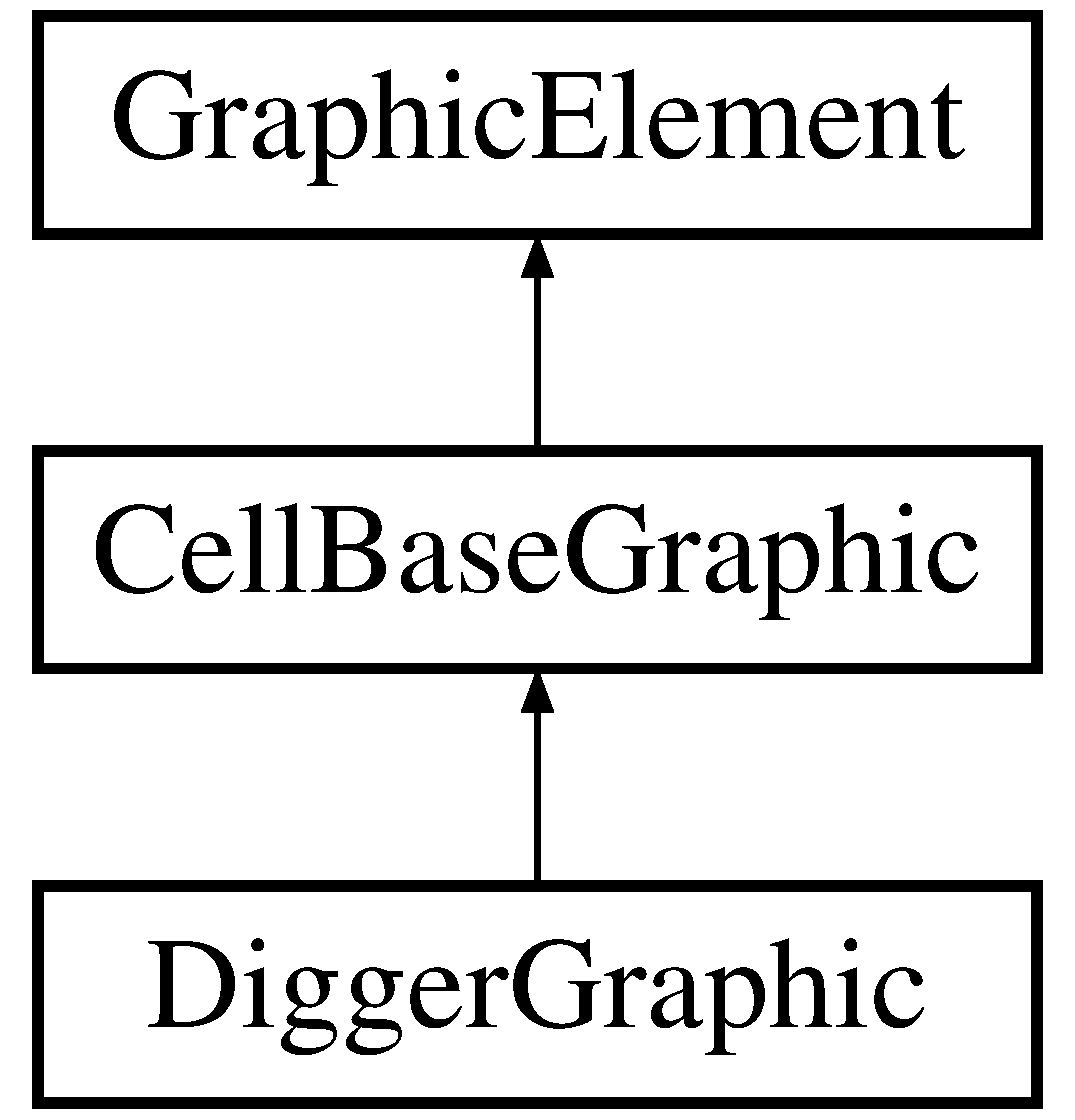
\includegraphics[height=3.000000cm]{class_digger_graphic}
\end{center}
\end{figure}
\subsection*{Fonctions membres publiques}
\begin{DoxyCompactItemize}
\item 
\hypertarget{class_digger_graphic_aa52f620e29aed04615addf75d9181eb5}{virtual void {\bfseries set\-Image\-To\-Sprite} ()}\label{class_digger_graphic_aa52f620e29aed04615addf75d9181eb5}

\end{DoxyCompactItemize}
\subsection*{Membres hérités additionnels}


La documentation de cette classe a été générée à partir des fichiers suivants \-:\begin{DoxyCompactItemize}
\item 
/\-Users/\-Ananas/\-Desktop/\-Mes\-Projets\-Git/purupurudigger/\-Code\-Cpp/Digger\-Graphic.\-h\item 
/\-Users/\-Ananas/\-Desktop/\-Mes\-Projets\-Git/purupurudigger/\-Code\-Cpp/Digger\-Graphic.\-cpp\end{DoxyCompactItemize}

\hypertarget{class_empty_cell}{\section{Référence de la classe Empty\-Cell}
\label{class_empty_cell}\index{Empty\-Cell@{Empty\-Cell}}
}


Classe modélisant ce qu'est une \hyperlink{class_empty_cell}{Empty\-Cell}.  




{\ttfamily \#include $<$Empty\-Cell.\-h$>$}

Graphe d'héritage de Empty\-Cell\-:\begin{figure}[H]
\begin{center}
\leavevmode
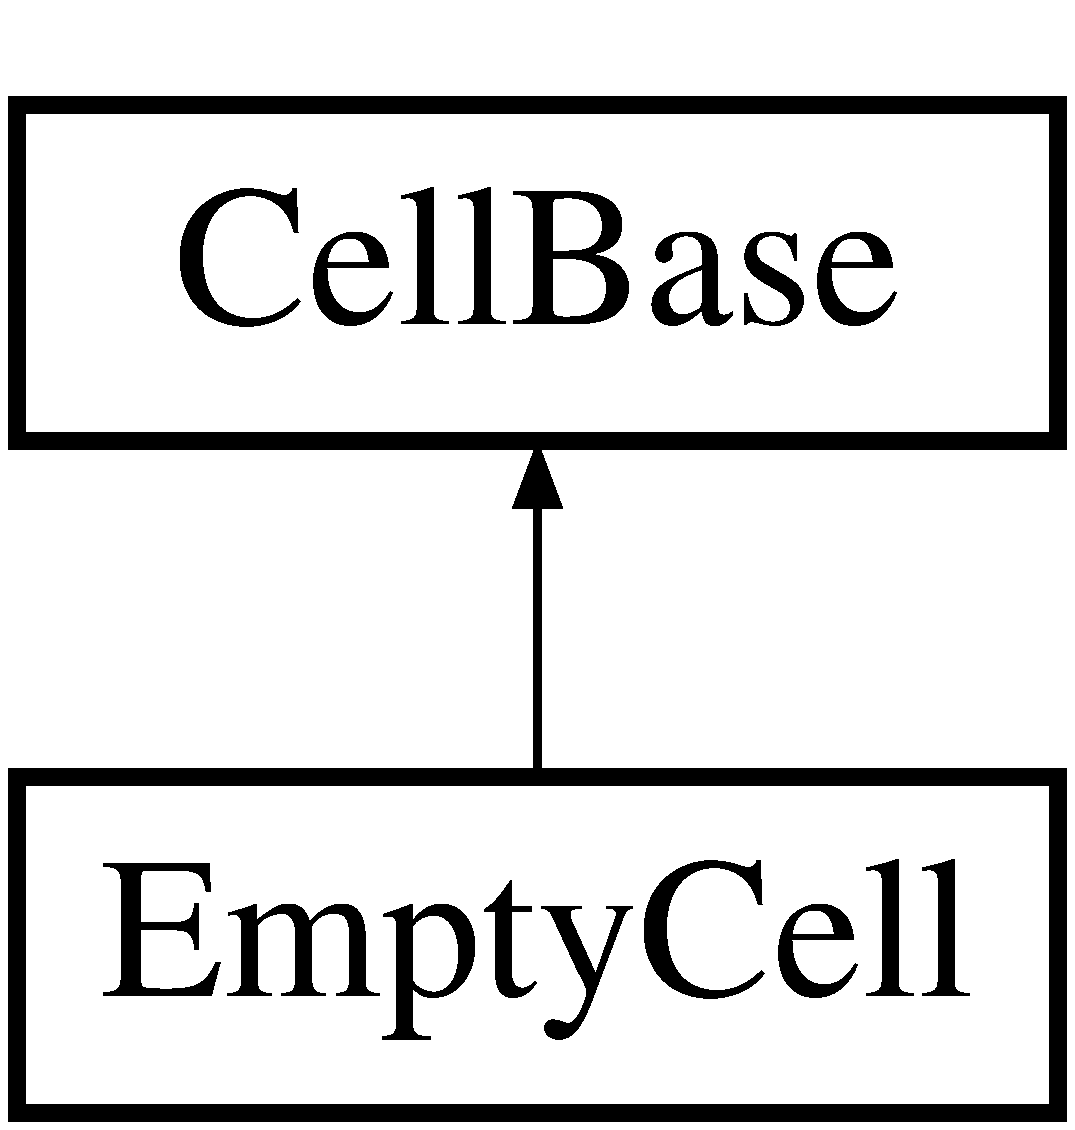
\includegraphics[height=2.000000cm]{class_empty_cell}
\end{center}
\end{figure}
\subsection*{Fonctions membres publiques}
\begin{DoxyCompactItemize}
\item 
\hyperlink{class_empty_cell_a1871cc46e277bf054e2fd9110f9030c3}{Empty\-Cell} ()
\begin{DoxyCompactList}\small\item\em Constructeur. \end{DoxyCompactList}\item 
\hyperlink{class_empty_cell_af51608a40bca4fb2d60be1882d7362da}{Empty\-Cell} (int x, int y)
\begin{DoxyCompactList}\small\item\em Constructeur paramétré \end{DoxyCompactList}\item 
\hyperlink{class_empty_cell_a888aa15c6c3dc2e882b42a78ee944432}{Empty\-Cell} (const \hyperlink{class_empty_cell}{Empty\-Cell} \&b)
\begin{DoxyCompactList}\small\item\em Constructeur par copie. \end{DoxyCompactList}\item 
virtual \hyperlink{class_empty_cell_a9a91934198895391fca6eac0b2fca9f5}{$\sim$\-Empty\-Cell} ()
\begin{DoxyCompactList}\small\item\em Destructeur. \end{DoxyCompactList}\item 
virtual \hyperlink{class_empty_cell}{Empty\-Cell} \& \hyperlink{class_empty_cell_a2b069d427ca55af2cba75382d8e7bb6f}{operator=} (const \hyperlink{class_empty_cell}{Empty\-Cell} \&b)
\begin{DoxyCompactList}\small\item\em Opérateur d'affectation pour recopier une case. \end{DoxyCompactList}\end{DoxyCompactItemize}
\subsection*{Membres hérités additionnels}


\subsection{Description détaillée}
Classe modélisant ce qu'est une \hyperlink{class_empty_cell}{Empty\-Cell}. 

\subsection{Documentation des constructeurs et destructeur}
\hypertarget{class_empty_cell_a1871cc46e277bf054e2fd9110f9030c3}{\index{Empty\-Cell@{Empty\-Cell}!Empty\-Cell@{Empty\-Cell}}
\index{Empty\-Cell@{Empty\-Cell}!EmptyCell@{Empty\-Cell}}
\subsubsection[{Empty\-Cell}]{\setlength{\rightskip}{0pt plus 5cm}Empty\-Cell\-::\-Empty\-Cell (
\begin{DoxyParamCaption}
{}
\end{DoxyParamCaption}
)}}\label{class_empty_cell_a1871cc46e277bf054e2fd9110f9030c3}


Constructeur. 

Constructeur de la classe \hyperlink{class_empty_cell}{Empty\-Cell} \hypertarget{class_empty_cell_af51608a40bca4fb2d60be1882d7362da}{\index{Empty\-Cell@{Empty\-Cell}!Empty\-Cell@{Empty\-Cell}}
\index{Empty\-Cell@{Empty\-Cell}!EmptyCell@{Empty\-Cell}}
\subsubsection[{Empty\-Cell}]{\setlength{\rightskip}{0pt plus 5cm}Empty\-Cell\-::\-Empty\-Cell (
\begin{DoxyParamCaption}
\item[{int}]{x, }
\item[{int}]{y}
\end{DoxyParamCaption}
)}}\label{class_empty_cell_af51608a40bca4fb2d60be1882d7362da}


Constructeur paramétré 

Constructeur paramétré de la classe \hyperlink{class_empty_cell}{Empty\-Cell} \hypertarget{class_empty_cell_a888aa15c6c3dc2e882b42a78ee944432}{\index{Empty\-Cell@{Empty\-Cell}!Empty\-Cell@{Empty\-Cell}}
\index{Empty\-Cell@{Empty\-Cell}!EmptyCell@{Empty\-Cell}}
\subsubsection[{Empty\-Cell}]{\setlength{\rightskip}{0pt plus 5cm}Empty\-Cell\-::\-Empty\-Cell (
\begin{DoxyParamCaption}
\item[{const {\bf Empty\-Cell} \&}]{b}
\end{DoxyParamCaption}
)}}\label{class_empty_cell_a888aa15c6c3dc2e882b42a78ee944432}


Constructeur par copie. 

Constructeur par copie de la classe \hyperlink{class_empty_cell}{Empty\-Cell} \hypertarget{class_empty_cell_a9a91934198895391fca6eac0b2fca9f5}{\index{Empty\-Cell@{Empty\-Cell}!$\sim$\-Empty\-Cell@{$\sim$\-Empty\-Cell}}
\index{$\sim$\-Empty\-Cell@{$\sim$\-Empty\-Cell}!EmptyCell@{Empty\-Cell}}
\subsubsection[{$\sim$\-Empty\-Cell}]{\setlength{\rightskip}{0pt plus 5cm}Empty\-Cell\-::$\sim$\-Empty\-Cell (
\begin{DoxyParamCaption}
{}
\end{DoxyParamCaption}
)\hspace{0.3cm}{\ttfamily [virtual]}}}\label{class_empty_cell_a9a91934198895391fca6eac0b2fca9f5}


Destructeur. 

Destructeur de la classe fille \hyperlink{class_empty_cell}{Empty\-Cell} 

\subsection{Documentation des fonctions membres}
\hypertarget{class_empty_cell_a2b069d427ca55af2cba75382d8e7bb6f}{\index{Empty\-Cell@{Empty\-Cell}!operator=@{operator=}}
\index{operator=@{operator=}!EmptyCell@{Empty\-Cell}}
\subsubsection[{operator=}]{\setlength{\rightskip}{0pt plus 5cm}{\bf Empty\-Cell} \& Empty\-Cell\-::operator= (
\begin{DoxyParamCaption}
\item[{const {\bf Empty\-Cell} \&}]{b}
\end{DoxyParamCaption}
)\hspace{0.3cm}{\ttfamily [virtual]}}}\label{class_empty_cell_a2b069d427ca55af2cba75382d8e7bb6f}


Opérateur d'affectation pour recopier une case. 


\begin{DoxyParams}{Paramètres}
{\em b\mbox{]}} & \hyperlink{class_empty_cell}{Empty\-Cell} b \-: opérateur d'affectation pour recopier une \hyperlink{class_empty_cell}{Empty\-Cell} \\
\hline
\end{DoxyParams}


La documentation de cette classe a été générée à partir des fichiers suivants \-:\begin{DoxyCompactItemize}
\item 
/\-Users/\-Ananas/\-Desktop/\-Mes\-Projets\-Git/purupurudigger/\-Code\-Cpp/\hyperlink{_empty_cell_8h}{Empty\-Cell.\-h}\item 
/\-Users/\-Ananas/\-Desktop/\-Mes\-Projets\-Git/purupurudigger/\-Code\-Cpp/\hyperlink{_empty_cell_8cpp}{Empty\-Cell.\-cpp}\end{DoxyCompactItemize}

\hypertarget{class_empty_graphic}{\section{Référence de la classe Empty\-Graphic}
\label{class_empty_graphic}\index{Empty\-Graphic@{Empty\-Graphic}}
}
Graphe d'héritage de Empty\-Graphic\-:\begin{figure}[H]
\begin{center}
\leavevmode
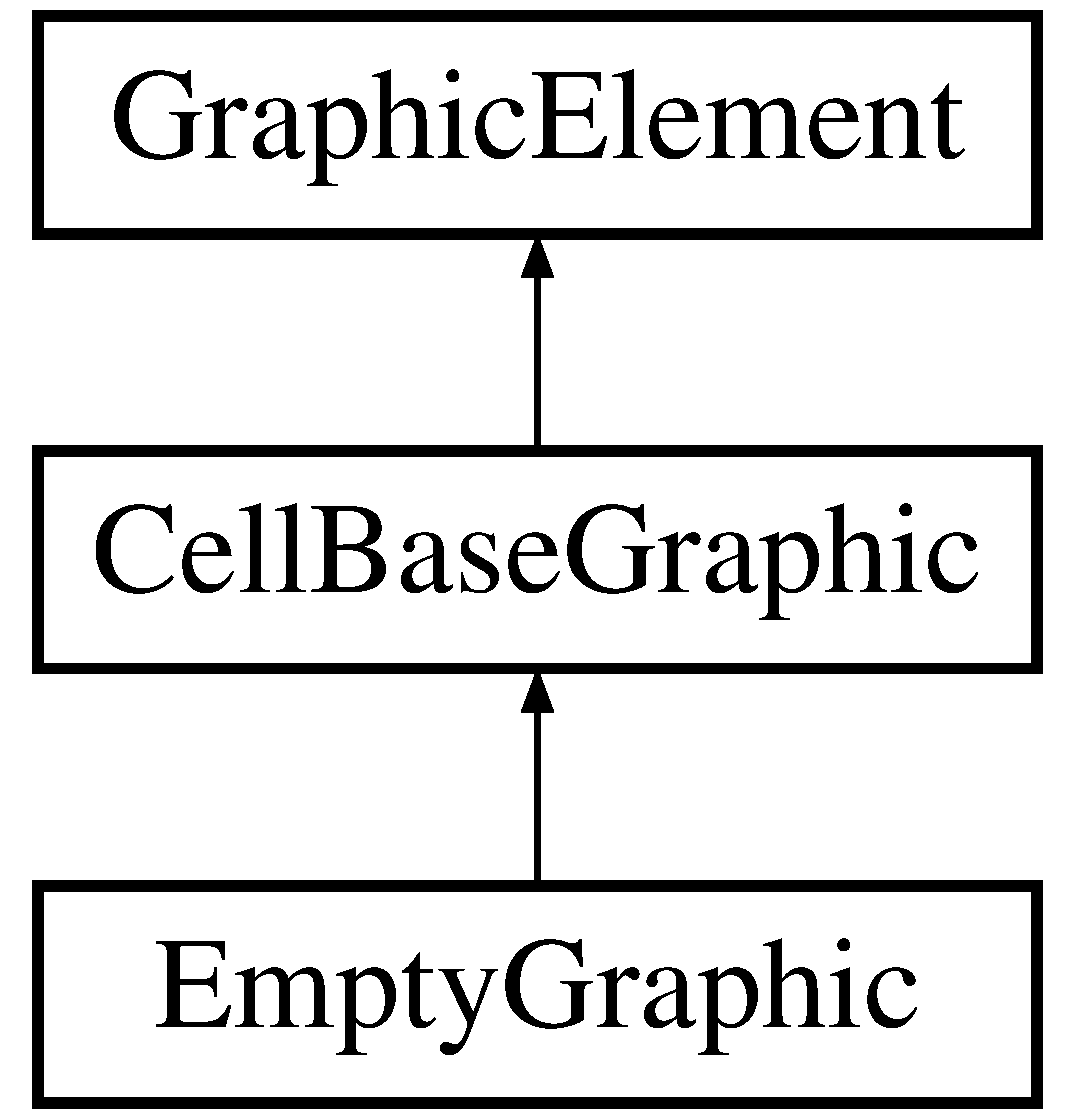
\includegraphics[height=3.000000cm]{class_empty_graphic}
\end{center}
\end{figure}
\subsection*{Fonctions membres publiques}
\begin{DoxyCompactItemize}
\item 
\hypertarget{class_empty_graphic_a39a2b103f1e102d21f6e3d464d09ee29}{virtual void {\bfseries set\-Image\-To\-Sprite} ()}\label{class_empty_graphic_a39a2b103f1e102d21f6e3d464d09ee29}

\end{DoxyCompactItemize}
\subsection*{Membres hérités additionnels}


La documentation de cette classe a été générée à partir des fichiers suivants \-:\begin{DoxyCompactItemize}
\item 
/\-Users/\-Ananas/\-Desktop/\-Mes\-Projets\-Git/purupurudigger/\-Code\-Cpp/Empty\-Graphic.\-h\item 
/\-Users/\-Ananas/\-Desktop/\-Mes\-Projets\-Git/purupurudigger/\-Code\-Cpp/Empty\-Graphic.\-cpp\end{DoxyCompactItemize}

\hypertarget{class_english_graphic}{\section{Référence de la classe English\-Graphic}
\label{class_english_graphic}\index{English\-Graphic@{English\-Graphic}}
}
Graphe d'héritage de English\-Graphic\-:\begin{figure}[H]
\begin{center}
\leavevmode
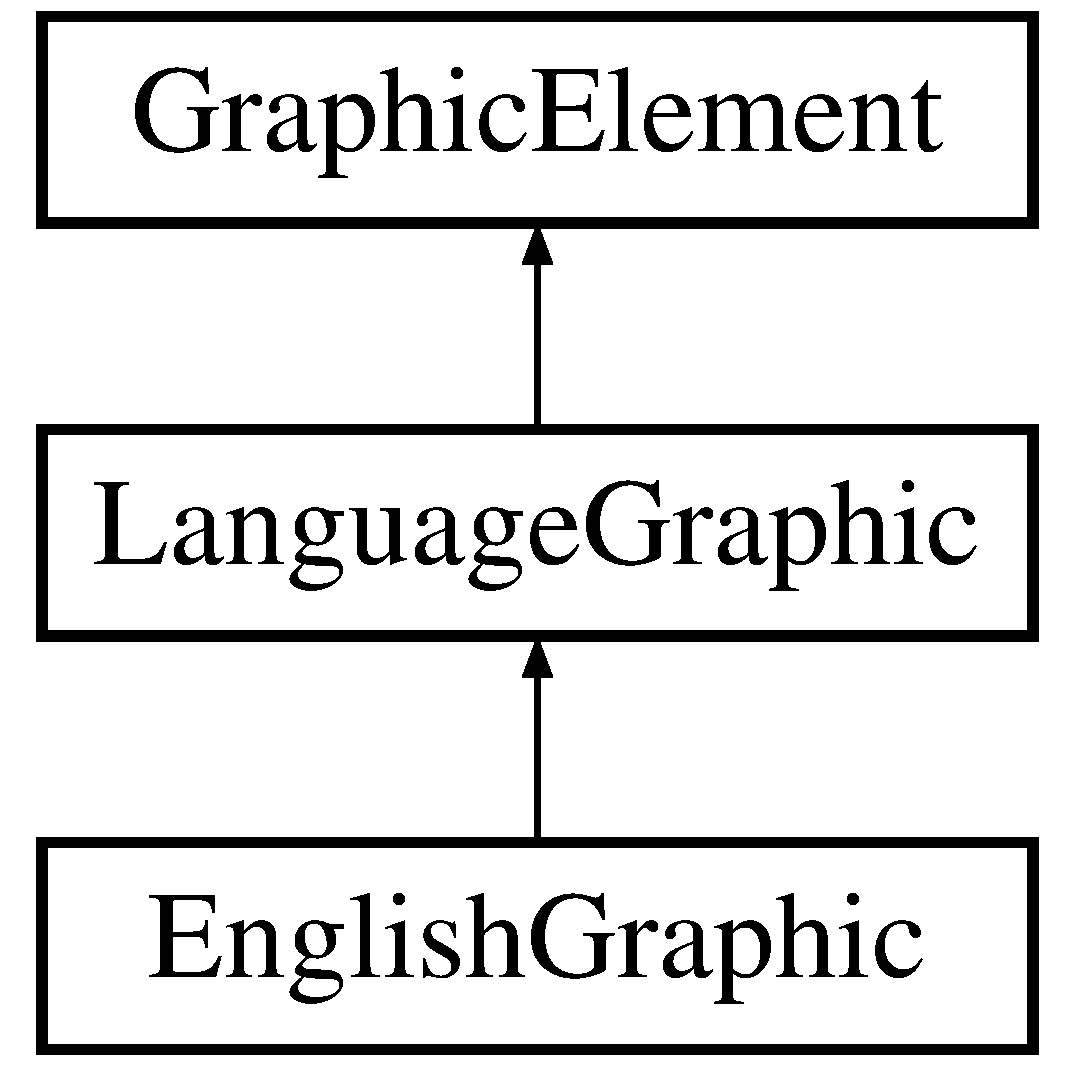
\includegraphics[height=3.000000cm]{class_english_graphic}
\end{center}
\end{figure}
\subsection*{Fonctions membres publiques}
\begin{DoxyCompactItemize}
\item 
\hypertarget{class_english_graphic_a8724406bc3e9168b6413683d5458a94a}{virtual void {\bfseries set\-Image\-To\-Sprite} ()}\label{class_english_graphic_a8724406bc3e9168b6413683d5458a94a}

\end{DoxyCompactItemize}
\subsection*{Membres hérités additionnels}


La documentation de cette classe a été générée à partir des fichiers suivants \-:\begin{DoxyCompactItemize}
\item 
/\-Users/\-Ananas/\-Desktop/\-Mes\-Projets\-Git/purupurudigger/\-Code\-Cpp/English\-Graphic.\-h\item 
/\-Users/\-Ananas/\-Desktop/\-Mes\-Projets\-Git/purupurudigger/\-Code\-Cpp/English\-Graphic.\-cpp\end{DoxyCompactItemize}

\hypertarget{class_french_graphic}{\section{Référence de la classe French\-Graphic}
\label{class_french_graphic}\index{French\-Graphic@{French\-Graphic}}
}
Graphe d'héritage de French\-Graphic\-:\begin{figure}[H]
\begin{center}
\leavevmode
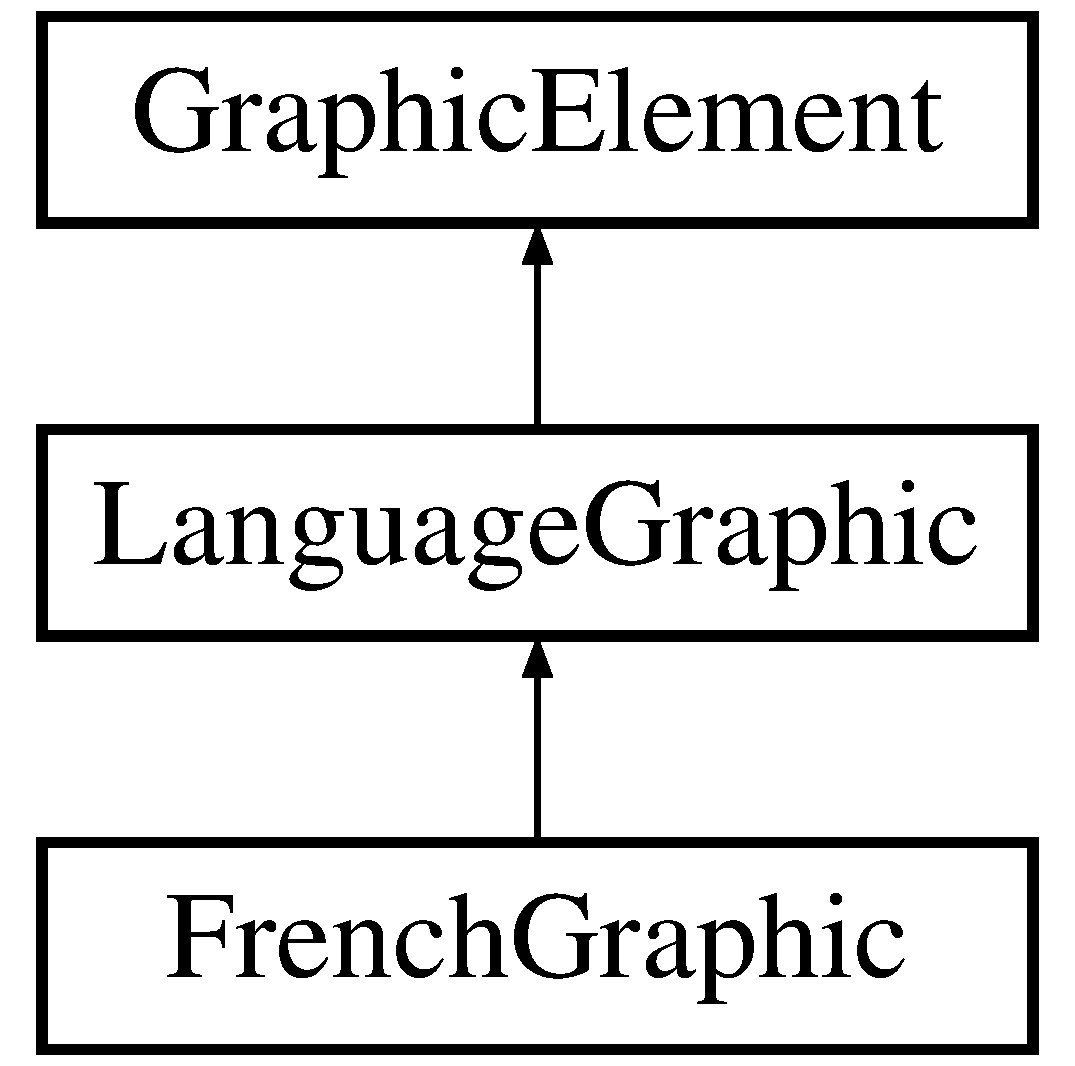
\includegraphics[height=3.000000cm]{class_french_graphic}
\end{center}
\end{figure}
\subsection*{Fonctions membres publiques}
\begin{DoxyCompactItemize}
\item 
\hypertarget{class_french_graphic_aedbd7c9da10afd3e9f4f6fa6251ffc5c}{virtual void {\bfseries set\-Image\-To\-Sprite} ()}\label{class_french_graphic_aedbd7c9da10afd3e9f4f6fa6251ffc5c}

\end{DoxyCompactItemize}
\subsection*{Membres hérités additionnels}


La documentation de cette classe a été générée à partir des fichiers suivants \-:\begin{DoxyCompactItemize}
\item 
/\-Users/\-Ananas/\-Desktop/\-Mes\-Projets\-Git/purupurudigger/\-Code\-Cpp/French\-Graphic.\-h\item 
/\-Users/\-Ananas/\-Desktop/\-Mes\-Projets\-Git/purupurudigger/\-Code\-Cpp/French\-Graphic.\-cpp\end{DoxyCompactItemize}

\hypertarget{class_game_model}{\section{Référence de la classe Game\-Model}
\label{class_game_model}\index{Game\-Model@{Game\-Model}}
}


Classe modélisant une partie.  




{\ttfamily \#include $<$Game\-Model.\-h$>$}

\subsection*{Fonctions membres publiques}
\begin{DoxyCompactItemize}
\item 
\hyperlink{class_game_model_aa5637be937d4a2ffe81541d513838424}{Game\-Model} ()
\begin{DoxyCompactList}\small\item\em Constructeur. \end{DoxyCompactList}\item 
\hyperlink{class_game_model_ac72de76e47bb6be675de3c49c15ac4af}{$\sim$\-Game\-Model} ()
\begin{DoxyCompactList}\small\item\em Destructeur. \end{DoxyCompactList}\item 
\hyperlink{class_score}{Score} $\ast$const \hyperlink{class_game_model_ab678951d954d7b978be043a045536d08}{get\-Score} ()
\begin{DoxyCompactList}\small\item\em Retourner notre score ( affichage ) \end{DoxyCompactList}\item 
\hyperlink{class_level}{Level} $\ast$const \hyperlink{class_game_model_aa7f4029f9ae959c7a1f07e263d92cccd}{get\-Level} ()
\begin{DoxyCompactList}\small\item\em Retourner notre \hyperlink{class_level}{Level} ( affichage ) \end{DoxyCompactList}\item 
void \hyperlink{class_game_model_aae26e8164a296410e518c1eae486da0a}{order\-Movement} (int depl)
\begin{DoxyCompactList}\small\item\em Ordonner un mouvement à notre grille. \end{DoxyCompactList}\item 
\hypertarget{class_game_model_a835e35b513c8598ea4143a74dcc08be4}{void {\bfseries order\-Movement} (int xclick, int yclick)}\label{class_game_model_a835e35b513c8598ea4143a74dcc08be4}

\item 
\hypertarget{class_game_model_a8fb77b55b8f6bd052c965a95cd82e2f2}{Movement {\bfseries get\-Movement} () const }\label{class_game_model_a8fb77b55b8f6bd052c965a95cd82e2f2}

\item 
bool \hyperlink{class_game_model_a0693b7716ee4a7307a0ac8b60a3fea52}{game\-Over} () const 
\begin{DoxyCompactList}\small\item\em Savoir si la partie est terminée. \end{DoxyCompactList}\item 
\hypertarget{class_game_model_aaaf0476b35dca74a9c786f523f011ba2}{void {\bfseries reset} ()}\label{class_game_model_aaaf0476b35dca74a9c786f523f011ba2}

\end{DoxyCompactItemize}


\subsection{Description détaillée}
Classe modélisant une partie. 

\subsection{Documentation des constructeurs et destructeur}
\hypertarget{class_game_model_aa5637be937d4a2ffe81541d513838424}{\index{Game\-Model@{Game\-Model}!Game\-Model@{Game\-Model}}
\index{Game\-Model@{Game\-Model}!GameModel@{Game\-Model}}
\subsubsection[{Game\-Model}]{\setlength{\rightskip}{0pt plus 5cm}Game\-Model\-::\-Game\-Model (
\begin{DoxyParamCaption}
{}
\end{DoxyParamCaption}
)}}\label{class_game_model_aa5637be937d4a2ffe81541d513838424}


Constructeur. 

Constructeur de la classe \hyperlink{class_game_model}{Game\-Model} \hypertarget{class_game_model_ac72de76e47bb6be675de3c49c15ac4af}{\index{Game\-Model@{Game\-Model}!$\sim$\-Game\-Model@{$\sim$\-Game\-Model}}
\index{$\sim$\-Game\-Model@{$\sim$\-Game\-Model}!GameModel@{Game\-Model}}
\subsubsection[{$\sim$\-Game\-Model}]{\setlength{\rightskip}{0pt plus 5cm}Game\-Model\-::$\sim$\-Game\-Model (
\begin{DoxyParamCaption}
{}
\end{DoxyParamCaption}
)}}\label{class_game_model_ac72de76e47bb6be675de3c49c15ac4af}


Destructeur. 

Destructeur de la classe \hyperlink{class_game_model}{Game\-Model} 

\subsection{Documentation des fonctions membres}
\hypertarget{class_game_model_a0693b7716ee4a7307a0ac8b60a3fea52}{\index{Game\-Model@{Game\-Model}!game\-Over@{game\-Over}}
\index{game\-Over@{game\-Over}!GameModel@{Game\-Model}}
\subsubsection[{game\-Over}]{\setlength{\rightskip}{0pt plus 5cm}bool Game\-Model\-::game\-Over (
\begin{DoxyParamCaption}
{}
\end{DoxyParamCaption}
) const}}\label{class_game_model_a0693b7716ee4a7307a0ac8b60a3fea52}


Savoir si la partie est terminée. 

\begin{DoxyReturn}{Renvoie}
true si la partie est finie 
\end{DoxyReturn}
\hypertarget{class_game_model_aa7f4029f9ae959c7a1f07e263d92cccd}{\index{Game\-Model@{Game\-Model}!get\-Level@{get\-Level}}
\index{get\-Level@{get\-Level}!GameModel@{Game\-Model}}
\subsubsection[{get\-Level}]{\setlength{\rightskip}{0pt plus 5cm}{\bf Level} $\ast$const Game\-Model\-::get\-Level (
\begin{DoxyParamCaption}
{}
\end{DoxyParamCaption}
)}}\label{class_game_model_aa7f4029f9ae959c7a1f07e263d92cccd}


Retourner notre \hyperlink{class_level}{Level} ( affichage ) 

\begin{DoxyReturn}{Renvoie}
un pointeur constant sur le level 
\end{DoxyReturn}
\hypertarget{class_game_model_ab678951d954d7b978be043a045536d08}{\index{Game\-Model@{Game\-Model}!get\-Score@{get\-Score}}
\index{get\-Score@{get\-Score}!GameModel@{Game\-Model}}
\subsubsection[{get\-Score}]{\setlength{\rightskip}{0pt plus 5cm}{\bf Score} $\ast$const Game\-Model\-::get\-Score (
\begin{DoxyParamCaption}
{}
\end{DoxyParamCaption}
)}}\label{class_game_model_ab678951d954d7b978be043a045536d08}


Retourner notre score ( affichage ) 

\begin{DoxyReturn}{Renvoie}
un pointeur constant sur le score 
\end{DoxyReturn}
\hypertarget{class_game_model_aae26e8164a296410e518c1eae486da0a}{\index{Game\-Model@{Game\-Model}!order\-Movement@{order\-Movement}}
\index{order\-Movement@{order\-Movement}!GameModel@{Game\-Model}}
\subsubsection[{order\-Movement}]{\setlength{\rightskip}{0pt plus 5cm}void Game\-Model\-::order\-Movement (
\begin{DoxyParamCaption}
\item[{int}]{depl}
\end{DoxyParamCaption}
)}}\label{class_game_model_aae26e8164a296410e518c1eae486da0a}


Ordonner un mouvement à notre grille. 


\begin{DoxyParams}[1]{Paramètres}
\mbox{\tt in}  & {\em le} & mouvement \\
\hline
\end{DoxyParams}


La documentation de cette classe a été générée à partir des fichiers suivants \-:\begin{DoxyCompactItemize}
\item 
/\-Users/\-Ananas/\-Desktop/\-Mes\-Projets\-Git/purupurudigger/\-Code\-Cpp/\hyperlink{_game_model_8h}{Game\-Model.\-h}\item 
/\-Users/\-Ananas/\-Desktop/\-Mes\-Projets\-Git/purupurudigger/\-Code\-Cpp/\hyperlink{_game_model_8cpp}{Game\-Model.\-cpp}\end{DoxyCompactItemize}

\hypertarget{class_game_view}{\section{Référence de la classe Game\-View}
\label{class_game_view}\index{Game\-View@{Game\-View}}
}


Classe modélisant ce qu'est une vue.  




{\ttfamily \#include $<$Game\-View.\-h$>$}

\subsection*{Fonctions membres publiques}
\begin{DoxyCompactItemize}
\item 
\hyperlink{class_game_view_a3851092ffd63639b4a498b70d279bdc0}{Game\-View} ()
\item 
void \hyperlink{class_game_view_a08a03be946eac62d5bdd9cd0e8262857}{set\-Model} (\hyperlink{class_game_model}{Game\-Model} $\ast$model)
\begin{DoxyCompactList}\small\item\em Injection du modèle à la vue. \end{DoxyCompactList}\item 
\hypertarget{class_game_view_aceb15f33e67a2b5ffc94c3bfbff50842}{void \hyperlink{class_game_view_aceb15f33e67a2b5ffc94c3bfbff50842}{treat\-Game} ()}\label{class_game_view_aceb15f33e67a2b5ffc94c3bfbff50842}

\begin{DoxyCompactList}\small\item\em La boucle de jeu. \end{DoxyCompactList}\item 
void \hyperlink{class_game_view_a08a03be946eac62d5bdd9cd0e8262857}{set\-Model} (\hyperlink{class_game_model}{Game\-Model} $\ast$model)
\begin{DoxyCompactList}\small\item\em Injection du modèle à la vue. \end{DoxyCompactList}\item 
\hypertarget{class_game_view_aceb15f33e67a2b5ffc94c3bfbff50842}{void \hyperlink{class_game_view_aceb15f33e67a2b5ffc94c3bfbff50842}{treat\-Game} ()}\label{class_game_view_aceb15f33e67a2b5ffc94c3bfbff50842}

\begin{DoxyCompactList}\small\item\em La boucle de jeu. \end{DoxyCompactList}\end{DoxyCompactItemize}


\subsection{Description détaillée}
Classe modélisant ce qu'est une vue. 

\subsection{Documentation des constructeurs et destructeur}
\hypertarget{class_game_view_a3851092ffd63639b4a498b70d279bdc0}{\index{Game\-View@{Game\-View}!Game\-View@{Game\-View}}
\index{Game\-View@{Game\-View}!GameView@{Game\-View}}
\subsubsection[{Game\-View}]{\setlength{\rightskip}{0pt plus 5cm}Game\-View\-::\-Game\-View (
\begin{DoxyParamCaption}
{}
\end{DoxyParamCaption}
)}}\label{class_game_view_a3851092ffd63639b4a498b70d279bdc0}
On set notre map pour l'affichage 

\subsection{Documentation des fonctions membres}
\hypertarget{class_game_view_a08a03be946eac62d5bdd9cd0e8262857}{\index{Game\-View@{Game\-View}!set\-Model@{set\-Model}}
\index{set\-Model@{set\-Model}!GameView@{Game\-View}}
\subsubsection[{set\-Model}]{\setlength{\rightskip}{0pt plus 5cm}void Game\-View\-::set\-Model (
\begin{DoxyParamCaption}
\item[{{\bf Game\-Model} $\ast$}]{model}
\end{DoxyParamCaption}
)}}\label{class_game_view_a08a03be946eac62d5bdd9cd0e8262857}


Injection du modèle à la vue. 

param\mbox{[}in\mbox{]} model \-: le modèle à interpréter \hypertarget{class_game_view_a08a03be946eac62d5bdd9cd0e8262857}{\index{Game\-View@{Game\-View}!set\-Model@{set\-Model}}
\index{set\-Model@{set\-Model}!GameView@{Game\-View}}
\subsubsection[{set\-Model}]{\setlength{\rightskip}{0pt plus 5cm}void Game\-View\-::set\-Model (
\begin{DoxyParamCaption}
\item[{{\bf Game\-Model} $\ast$}]{model}
\end{DoxyParamCaption}
)}}\label{class_game_view_a08a03be946eac62d5bdd9cd0e8262857}


Injection du modèle à la vue. 

param\mbox{[}in\mbox{]} model \-: le modèle à interpréter 

La documentation de cette classe a été générée à partir des fichiers suivants \-:\begin{DoxyCompactItemize}
\item 
/\-Users/\-Ananas/\-Desktop/\-Mes\-Projets\-Git/purupurudigger/\-Code\-Cpp/\hyperlink{_game_view_8h}{Game\-View.\-h}\item 
/\-Users/\-Ananas/\-Desktop/\-Mes\-Projets\-Git/purupurudigger/\-Code\-Cpp/Game\-View\-S\-F\-M\-L.\-h\item 
/\-Users/\-Ananas/\-Desktop/\-Mes\-Projets\-Git/purupurudigger/\-Code\-Cpp/\hyperlink{_game_view_8cpp}{Game\-View.\-cpp}\item 
/\-Users/\-Ananas/\-Desktop/\-Mes\-Projets\-Git/purupurudigger/\-Code\-Cpp/Game\-View\-S\-F\-M\-L.\-cpp\end{DoxyCompactItemize}

\hypertarget{class_gold_cell}{\section{Référence de la classe Gold\-Cell}
\label{class_gold_cell}\index{Gold\-Cell@{Gold\-Cell}}
}


Classe modélisant ce qu'est une \hyperlink{class_gold_cell}{Gold\-Cell}.  




{\ttfamily \#include $<$Gold\-Cell.\-h$>$}

Graphe d'héritage de Gold\-Cell\-:\begin{figure}[H]
\begin{center}
\leavevmode
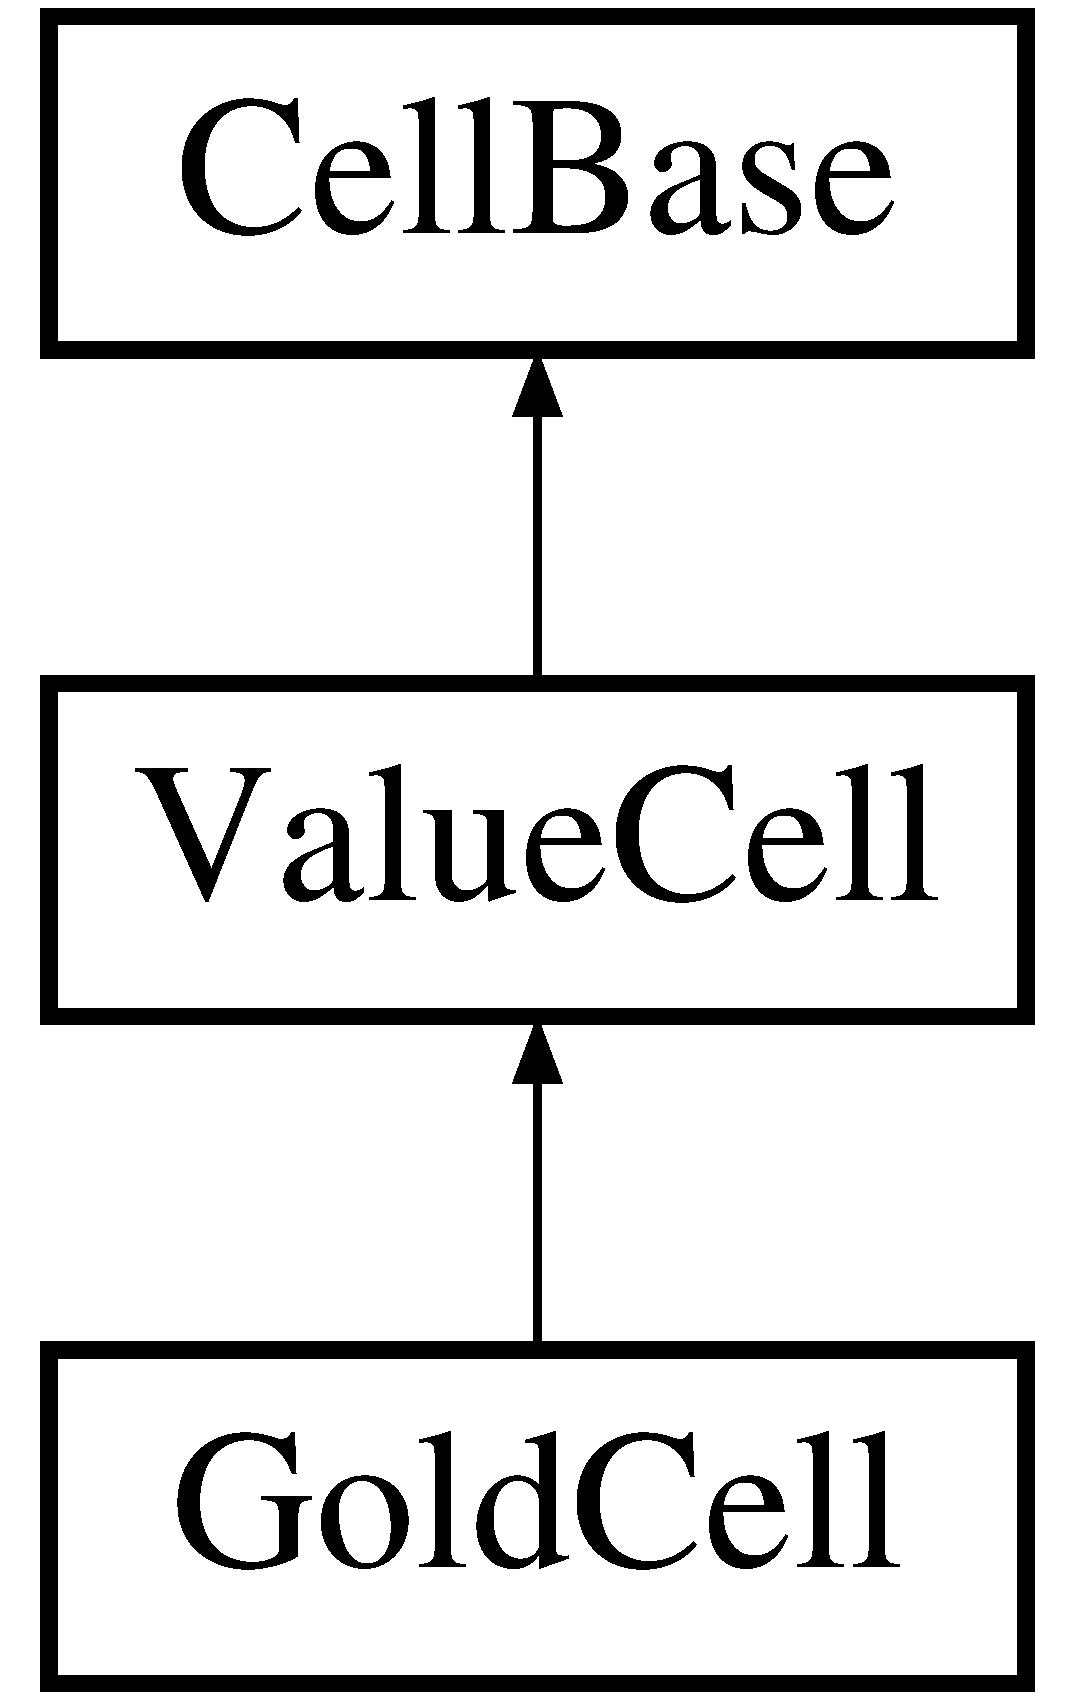
\includegraphics[height=3.000000cm]{class_gold_cell}
\end{center}
\end{figure}
\subsection*{Fonctions membres publiques}
\begin{DoxyCompactItemize}
\item 
\hyperlink{class_gold_cell_ae7b344911cc3027935f0f9142e05d184}{Gold\-Cell} ()
\begin{DoxyCompactList}\small\item\em Constructeur. \end{DoxyCompactList}\item 
\hyperlink{class_gold_cell_a3bff4553728b09dd6aa1a1a27961eea7}{Gold\-Cell} (int x, int y)
\begin{DoxyCompactList}\small\item\em Constructeur paramétré \end{DoxyCompactList}\item 
\hyperlink{class_gold_cell_abac5d2fdba9d335d4e59866228381b6b}{Gold\-Cell} (const \hyperlink{class_gold_cell}{Gold\-Cell} \&g)
\begin{DoxyCompactList}\small\item\em Constructeur par copie. \end{DoxyCompactList}\item 
virtual \hyperlink{class_gold_cell_a385e8c1656defcd6063c955db8869d87}{$\sim$\-Gold\-Cell} ()
\begin{DoxyCompactList}\small\item\em Destructeur. \end{DoxyCompactList}\item 
virtual int \hyperlink{class_gold_cell_a1f111db9bdb520176a48bb689c7baf2b}{get\-Points} () const 
\begin{DoxyCompactList}\small\item\em Retourne les points que va ajouter la case dans les scores. \end{DoxyCompactList}\item 
virtual \hyperlink{class_gold_cell}{Gold\-Cell} \& \hyperlink{class_gold_cell_ac858c489397f874d2091d2987a321cfa}{operator=} (const \hyperlink{class_gold_cell}{Gold\-Cell} \&g)
\begin{DoxyCompactList}\small\item\em Opérateur d'affectation pour recopier une \hyperlink{class_gold_cell}{Gold\-Cell}. \end{DoxyCompactList}\end{DoxyCompactItemize}
\subsection*{Membres hérités additionnels}


\subsection{Description détaillée}
Classe modélisant ce qu'est une \hyperlink{class_gold_cell}{Gold\-Cell}. 

\subsection{Documentation des constructeurs et destructeur}
\hypertarget{class_gold_cell_ae7b344911cc3027935f0f9142e05d184}{\index{Gold\-Cell@{Gold\-Cell}!Gold\-Cell@{Gold\-Cell}}
\index{Gold\-Cell@{Gold\-Cell}!GoldCell@{Gold\-Cell}}
\subsubsection[{Gold\-Cell}]{\setlength{\rightskip}{0pt plus 5cm}Gold\-Cell\-::\-Gold\-Cell (
\begin{DoxyParamCaption}
{}
\end{DoxyParamCaption}
)}}\label{class_gold_cell_ae7b344911cc3027935f0f9142e05d184}


Constructeur. 

Constructeur de la classe \hyperlink{class_gold_cell}{Gold\-Cell} \hypertarget{class_gold_cell_a3bff4553728b09dd6aa1a1a27961eea7}{\index{Gold\-Cell@{Gold\-Cell}!Gold\-Cell@{Gold\-Cell}}
\index{Gold\-Cell@{Gold\-Cell}!GoldCell@{Gold\-Cell}}
\subsubsection[{Gold\-Cell}]{\setlength{\rightskip}{0pt plus 5cm}Gold\-Cell\-::\-Gold\-Cell (
\begin{DoxyParamCaption}
\item[{int}]{x, }
\item[{int}]{y}
\end{DoxyParamCaption}
)}}\label{class_gold_cell_a3bff4553728b09dd6aa1a1a27961eea7}


Constructeur paramétré 

Constructeur paramétré de la classe \hyperlink{class_gold_cell}{Gold\-Cell} \hypertarget{class_gold_cell_abac5d2fdba9d335d4e59866228381b6b}{\index{Gold\-Cell@{Gold\-Cell}!Gold\-Cell@{Gold\-Cell}}
\index{Gold\-Cell@{Gold\-Cell}!GoldCell@{Gold\-Cell}}
\subsubsection[{Gold\-Cell}]{\setlength{\rightskip}{0pt plus 5cm}Gold\-Cell\-::\-Gold\-Cell (
\begin{DoxyParamCaption}
\item[{const {\bf Gold\-Cell} \&}]{g}
\end{DoxyParamCaption}
)}}\label{class_gold_cell_abac5d2fdba9d335d4e59866228381b6b}


Constructeur par copie. 


\begin{DoxyParams}[1]{Paramètres}
\mbox{\tt in}  & {\em \hyperlink{class_gold_cell}{Gold\-Cell}} & g \\
\hline
\mbox{\tt out}  & {\em \hyperlink{class_gold_cell}{Gold\-Cell}} & g \\
\hline
\end{DoxyParams}
\hypertarget{class_gold_cell_a385e8c1656defcd6063c955db8869d87}{\index{Gold\-Cell@{Gold\-Cell}!$\sim$\-Gold\-Cell@{$\sim$\-Gold\-Cell}}
\index{$\sim$\-Gold\-Cell@{$\sim$\-Gold\-Cell}!GoldCell@{Gold\-Cell}}
\subsubsection[{$\sim$\-Gold\-Cell}]{\setlength{\rightskip}{0pt plus 5cm}Gold\-Cell\-::$\sim$\-Gold\-Cell (
\begin{DoxyParamCaption}
{}
\end{DoxyParamCaption}
)\hspace{0.3cm}{\ttfamily [virtual]}}}\label{class_gold_cell_a385e8c1656defcd6063c955db8869d87}


Destructeur. 

Destructeur de la classe fille \hyperlink{class_gold_cell}{Gold\-Cell} 

\subsection{Documentation des fonctions membres}
\hypertarget{class_gold_cell_a1f111db9bdb520176a48bb689c7baf2b}{\index{Gold\-Cell@{Gold\-Cell}!get\-Points@{get\-Points}}
\index{get\-Points@{get\-Points}!GoldCell@{Gold\-Cell}}
\subsubsection[{get\-Points}]{\setlength{\rightskip}{0pt plus 5cm}int Gold\-Cell\-::get\-Points (
\begin{DoxyParamCaption}
{}
\end{DoxyParamCaption}
) const\hspace{0.3cm}{\ttfamily [virtual]}}}\label{class_gold_cell_a1f111db9bdb520176a48bb689c7baf2b}


Retourne les points que va ajouter la case dans les scores. 

\begin{DoxyReturn}{Renvoie}
my\-\_\-points, retourne la valeur de la case 
\end{DoxyReturn}


Réimplémentée à partir de \hyperlink{class_value_cell_a711326876009350576251e512fcf126e}{Value\-Cell}.

\hypertarget{class_gold_cell_ac858c489397f874d2091d2987a321cfa}{\index{Gold\-Cell@{Gold\-Cell}!operator=@{operator=}}
\index{operator=@{operator=}!GoldCell@{Gold\-Cell}}
\subsubsection[{operator=}]{\setlength{\rightskip}{0pt plus 5cm}{\bf Gold\-Cell} \& Gold\-Cell\-::operator= (
\begin{DoxyParamCaption}
\item[{const {\bf Gold\-Cell} \&}]{g}
\end{DoxyParamCaption}
)\hspace{0.3cm}{\ttfamily [virtual]}}}\label{class_gold_cell_ac858c489397f874d2091d2987a321cfa}


Opérateur d'affectation pour recopier une \hyperlink{class_gold_cell}{Gold\-Cell}. 


\begin{DoxyParams}[1]{Paramètres}
\mbox{\tt in}  & {\em \hyperlink{class_gold_cell}{Gold\-Cell}} & g \-: opérateur d'affectation pour recopier une \hyperlink{class_gold_cell}{Gold\-Cell} \\
\hline
\end{DoxyParams}


La documentation de cette classe a été générée à partir des fichiers suivants \-:\begin{DoxyCompactItemize}
\item 
/\-Users/\-Ananas/\-Desktop/\-Mes\-Projets\-Git/purupurudigger/\-Code\-Cpp/\hyperlink{_gold_cell_8h}{Gold\-Cell.\-h}\item 
/\-Users/\-Ananas/\-Desktop/\-Mes\-Projets\-Git/purupurudigger/\-Code\-Cpp/\hyperlink{_gold_cell_8cpp}{Gold\-Cell.\-cpp}\end{DoxyCompactItemize}

\hypertarget{class_gold_graphic}{\section{Référence de la classe Gold\-Graphic}
\label{class_gold_graphic}\index{Gold\-Graphic@{Gold\-Graphic}}
}
Graphe d'héritage de Gold\-Graphic\-:\begin{figure}[H]
\begin{center}
\leavevmode
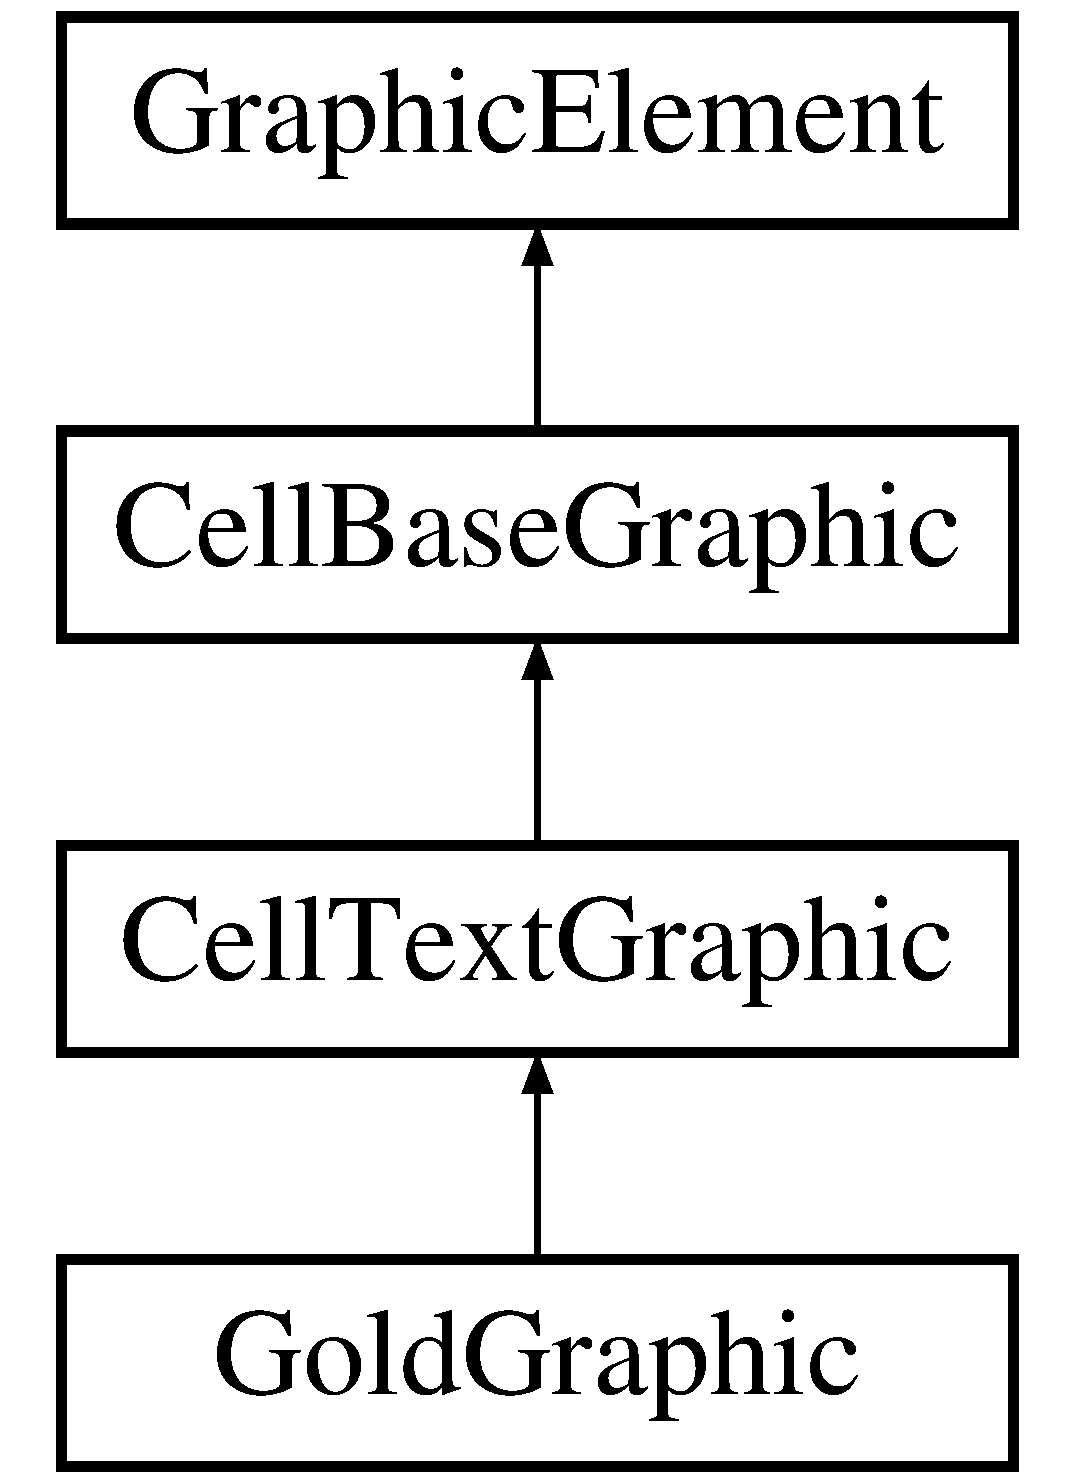
\includegraphics[height=4.000000cm]{class_gold_graphic}
\end{center}
\end{figure}
\subsection*{Fonctions membres publiques}
\begin{DoxyCompactItemize}
\item 
\hypertarget{class_gold_graphic_a6375496c97a1dd0e0b2d9241add4167c}{virtual void {\bfseries set\-Image\-To\-Sprite} ()}\label{class_gold_graphic_a6375496c97a1dd0e0b2d9241add4167c}

\end{DoxyCompactItemize}
\subsection*{Membres hérités additionnels}


La documentation de cette classe a été générée à partir des fichiers suivants \-:\begin{DoxyCompactItemize}
\item 
/\-Users/\-Ananas/\-Desktop/\-Mes\-Projets\-Git/purupurudigger/\-Code\-Cpp/Gold\-Graphic.\-h\item 
/\-Users/\-Ananas/\-Desktop/\-Mes\-Projets\-Git/purupurudigger/\-Code\-Cpp/Gold\-Graphic.\-cpp\end{DoxyCompactItemize}

\hypertarget{class_graphic_audible_element}{\section{Référence de la classe Graphic\-Audible\-Element}
\label{class_graphic_audible_element}\index{Graphic\-Audible\-Element@{Graphic\-Audible\-Element}}
}
Graphe d'héritage de Graphic\-Audible\-Element\-:\begin{figure}[H]
\begin{center}
\leavevmode
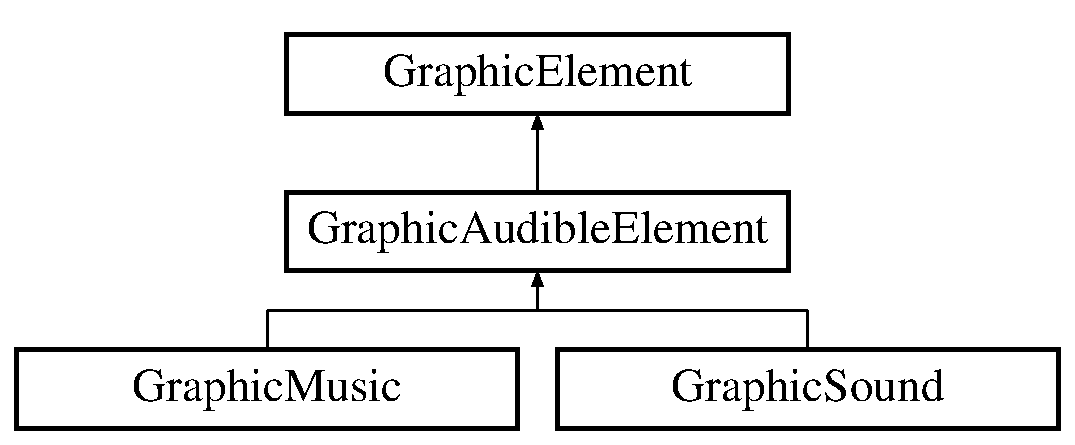
\includegraphics[height=3.000000cm]{class_graphic_audible_element}
\end{center}
\end{figure}
\subsection*{Fonctions membres publiques}
\begin{DoxyCompactItemize}
\item 
\hypertarget{class_graphic_audible_element_a77fd0f4aa0bf4e9297a790a1e920a00d}{virtual void {\bfseries set\-Image\-To\-Sprite} ()}\label{class_graphic_audible_element_a77fd0f4aa0bf4e9297a790a1e920a00d}

\item 
\hypertarget{class_graphic_audible_element_a0c740dab12b2f82088fa3e9ef700b97d}{virtual void {\bfseries set\-Teacher\-Mode} ()}\label{class_graphic_audible_element_a0c740dab12b2f82088fa3e9ef700b97d}

\item 
\hypertarget{class_graphic_audible_element_a02916f15862524394c0ab8af1aed1b26}{virtual void {\bfseries set\-Ananas\-Mode} ()}\label{class_graphic_audible_element_a02916f15862524394c0ab8af1aed1b26}

\item 
\hypertarget{class_graphic_audible_element_a26b22e8494b6bc40258692b8d79b33ba}{virtual void {\bfseries reverse} ()=0}\label{class_graphic_audible_element_a26b22e8494b6bc40258692b8d79b33ba}

\item 
\hypertarget{class_graphic_audible_element_a6ea54ae9948bed795527b42e3bbfc69a}{bool {\bfseries get\-On\-Off} () const }\label{class_graphic_audible_element_a6ea54ae9948bed795527b42e3bbfc69a}

\end{DoxyCompactItemize}
\subsection*{Attributs protégés}
\begin{DoxyCompactItemize}
\item 
\hypertarget{class_graphic_audible_element_ab0393a89bf30f2ff574b38cc09241ba4}{bool {\bfseries is\-On}}\label{class_graphic_audible_element_ab0393a89bf30f2ff574b38cc09241ba4}

\end{DoxyCompactItemize}
\subsection*{Attributs protégés statiques}
\begin{DoxyCompactItemize}
\item 
\hypertarget{class_graphic_audible_element_accfc407868d33341460d3272561b15d3}{static sf\-::\-Image {\bfseries my\-\_\-image}}\label{class_graphic_audible_element_accfc407868d33341460d3272561b15d3}

\end{DoxyCompactItemize}


La documentation de cette classe a été générée à partir des fichiers suivants \-:\begin{DoxyCompactItemize}
\item 
/\-Users/\-Ananas/\-Desktop/\-Mes\-Projets\-Git/purupurudigger/\-Code\-Cpp/Graphic\-Audible\-Element.\-h\item 
/\-Users/\-Ananas/\-Desktop/\-Mes\-Projets\-Git/purupurudigger/\-Code\-Cpp/Graphic\-Audible\-Element.\-cpp\end{DoxyCompactItemize}

\hypertarget{class_graphic_element}{\section{Référence de la classe Graphic\-Element}
\label{class_graphic_element}\index{Graphic\-Element@{Graphic\-Element}}
}
Graphe d'héritage de Graphic\-Element\-:\begin{figure}[H]
\begin{center}
\leavevmode
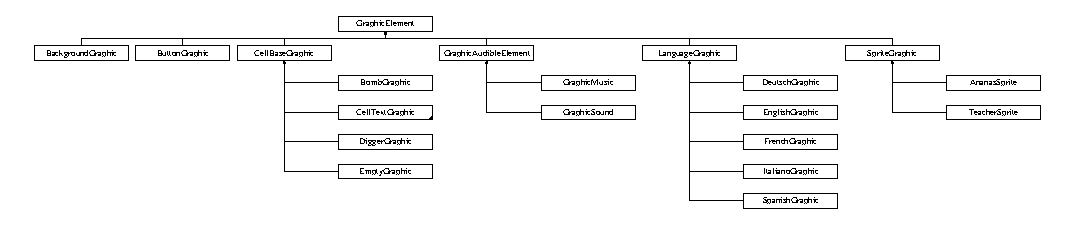
\includegraphics[height=2.578947cm]{class_graphic_element}
\end{center}
\end{figure}
\subsection*{Fonctions membres publiques}
\begin{DoxyCompactItemize}
\item 
\hypertarget{class_graphic_element_a236fbf61e8623a79c3ba3c154e8ebcdc}{virtual void {\bfseries set\-Teacher\-Mode} ()=0}\label{class_graphic_element_a236fbf61e8623a79c3ba3c154e8ebcdc}

\item 
\hypertarget{class_graphic_element_a8380da6f1b3db8d3bb1280b29f0a8e3c}{virtual void {\bfseries set\-Ananas\-Mode} ()=0}\label{class_graphic_element_a8380da6f1b3db8d3bb1280b29f0a8e3c}

\item 
\hypertarget{class_graphic_element_a36f73fee3d4548034a453ac48f80f102}{virtual void {\bfseries set\-Image\-To\-Sprite} ()=0}\label{class_graphic_element_a36f73fee3d4548034a453ac48f80f102}

\item 
\hypertarget{class_graphic_element_a7eb43ee4425ba80ea9865635c0f2e068}{virtual void {\bfseries set\-Sprite\-And\-Draw} (int x, int y, sf\-::\-Render\-Window $\ast$\-\_\-window)}\label{class_graphic_element_a7eb43ee4425ba80ea9865635c0f2e068}

\item 
\hypertarget{class_graphic_element_aadeb26c2c6e4f565b539da573c5c72c4}{virtual void {\bfseries draw} (sf\-::\-Render\-Window $\ast$\-\_\-window) const }\label{class_graphic_element_aadeb26c2c6e4f565b539da573c5c72c4}

\item 
\hypertarget{class_graphic_element_abb979d8b0590a0fc548a7698146179a2}{bool {\bfseries is\-In\-Zone} (int x, int y) const }\label{class_graphic_element_abb979d8b0590a0fc548a7698146179a2}

\item 
\hypertarget{class_graphic_element_a54dac49064cff360b8c5f97bfc66b9e3}{int {\bfseries get\-X\-Pos} () const }\label{class_graphic_element_a54dac49064cff360b8c5f97bfc66b9e3}

\item 
\hypertarget{class_graphic_element_abec2c4fe9aed0bb58b3b16747f9cbe3a}{int {\bfseries get\-Y\-Pos} () const }\label{class_graphic_element_abec2c4fe9aed0bb58b3b16747f9cbe3a}

\end{DoxyCompactItemize}
\subsection*{Attributs protégés}
\begin{DoxyCompactItemize}
\item 
\hypertarget{class_graphic_element_a4dc07a8f4481911bfe363bbf6f0b669a}{sf\-::\-Sprite {\bfseries my\-\_\-sprite}}\label{class_graphic_element_a4dc07a8f4481911bfe363bbf6f0b669a}

\end{DoxyCompactItemize}


La documentation de cette classe a été générée à partir des fichiers suivants \-:\begin{DoxyCompactItemize}
\item 
/\-Users/\-Ananas/\-Desktop/\-Mes\-Projets\-Git/purupurudigger/\-Code\-Cpp/Graphic\-Element.\-h\item 
/\-Users/\-Ananas/\-Desktop/\-Mes\-Projets\-Git/purupurudigger/\-Code\-Cpp/Graphic\-Element.\-cpp\end{DoxyCompactItemize}

\hypertarget{class_graphic_music}{\section{Référence de la classe Graphic\-Music}
\label{class_graphic_music}\index{Graphic\-Music@{Graphic\-Music}}
}
Graphe d'héritage de Graphic\-Music\-:\begin{figure}[H]
\begin{center}
\leavevmode
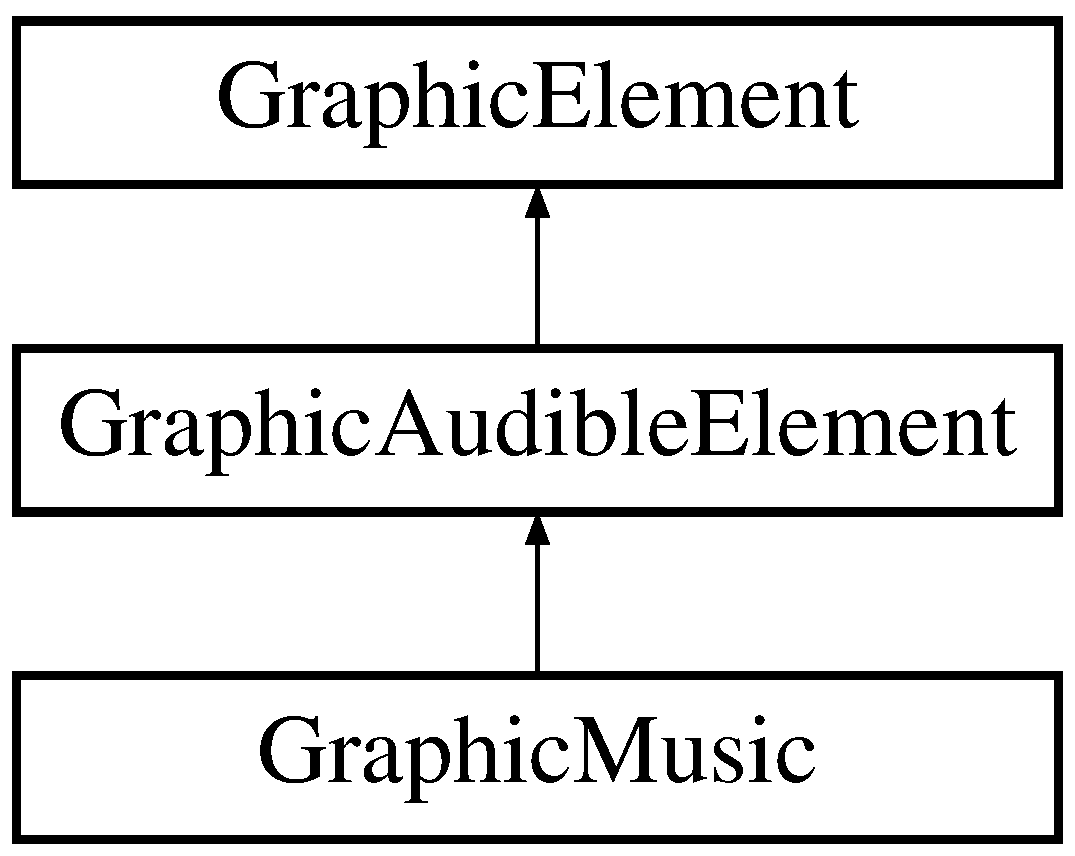
\includegraphics[height=3.000000cm]{class_graphic_music}
\end{center}
\end{figure}
\subsection*{Fonctions membres publiques}
\begin{DoxyCompactItemize}
\item 
\hypertarget{class_graphic_music_a0528a4869bf1d97b2b7e0a7f8b0029f1}{virtual void {\bfseries set\-Image\-To\-Sprite} ()}\label{class_graphic_music_a0528a4869bf1d97b2b7e0a7f8b0029f1}

\item 
\hypertarget{class_graphic_music_af3f690eaed25bdd2e5598a6f6ad5558c}{virtual void {\bfseries reverse} ()}\label{class_graphic_music_af3f690eaed25bdd2e5598a6f6ad5558c}

\end{DoxyCompactItemize}
\subsection*{Membres hérités additionnels}


La documentation de cette classe a été générée à partir des fichiers suivants \-:\begin{DoxyCompactItemize}
\item 
/\-Users/\-Ananas/\-Desktop/\-Mes\-Projets\-Git/purupurudigger/\-Code\-Cpp/Graphic\-Music.\-h\item 
/\-Users/\-Ananas/\-Desktop/\-Mes\-Projets\-Git/purupurudigger/\-Code\-Cpp/Graphic\-Music.\-cpp\end{DoxyCompactItemize}

\hypertarget{class_graphic_sound}{\section{Référence de la classe Graphic\-Sound}
\label{class_graphic_sound}\index{Graphic\-Sound@{Graphic\-Sound}}
}
Graphe d'héritage de Graphic\-Sound\-:\begin{figure}[H]
\begin{center}
\leavevmode
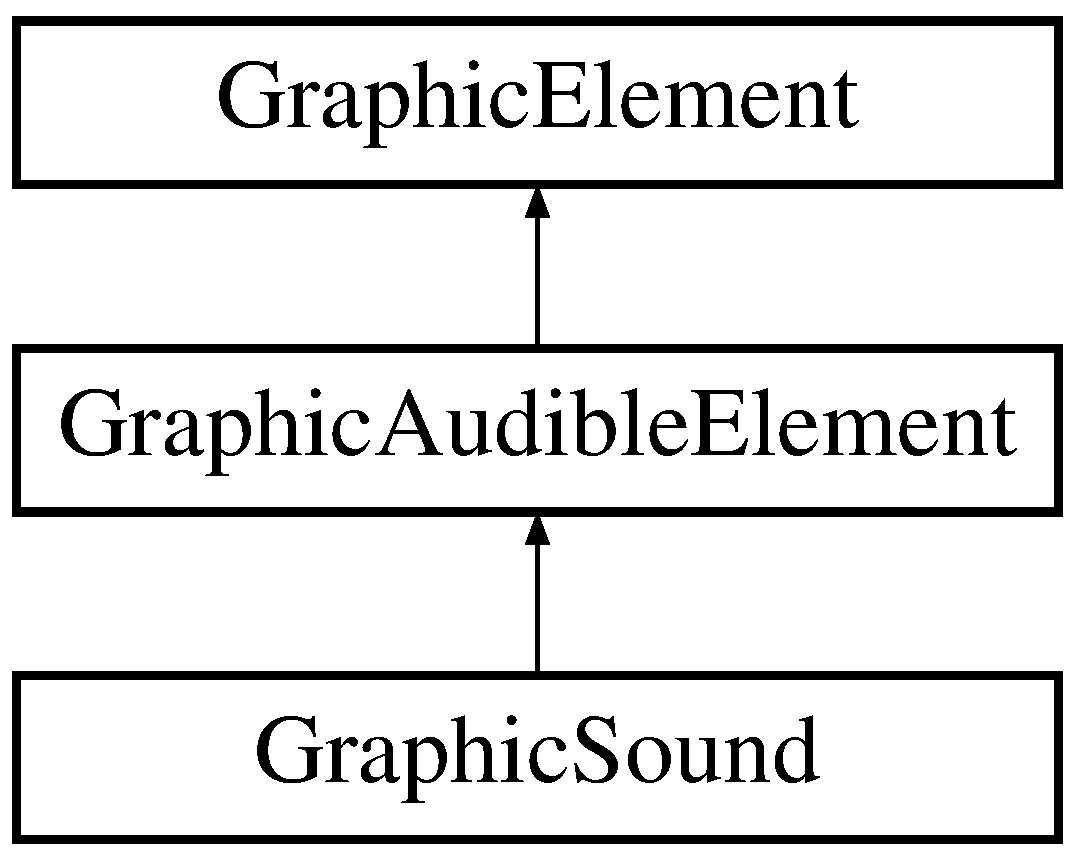
\includegraphics[height=3.000000cm]{class_graphic_sound}
\end{center}
\end{figure}
\subsection*{Fonctions membres publiques}
\begin{DoxyCompactItemize}
\item 
\hypertarget{class_graphic_sound_a2d2cd8f4d8494ec67a82d17aa7e40551}{virtual void {\bfseries set\-Image\-To\-Sprite} ()}\label{class_graphic_sound_a2d2cd8f4d8494ec67a82d17aa7e40551}

\item 
\hypertarget{class_graphic_sound_a45c58758081239bd45bc6b03eaea8989}{virtual void {\bfseries reverse} ()}\label{class_graphic_sound_a45c58758081239bd45bc6b03eaea8989}

\end{DoxyCompactItemize}
\subsection*{Membres hérités additionnels}


La documentation de cette classe a été générée à partir des fichiers suivants \-:\begin{DoxyCompactItemize}
\item 
/\-Users/\-Ananas/\-Desktop/\-Mes\-Projets\-Git/purupurudigger/\-Code\-Cpp/Graphic\-Sound.\-h\item 
/\-Users/\-Ananas/\-Desktop/\-Mes\-Projets\-Git/purupurudigger/\-Code\-Cpp/Graphic\-Sound.\-cpp\end{DoxyCompactItemize}

\hypertarget{class_italiano_graphic}{\section{Référence de la classe Italiano\-Graphic}
\label{class_italiano_graphic}\index{Italiano\-Graphic@{Italiano\-Graphic}}
}
Graphe d'héritage de Italiano\-Graphic\-:\begin{figure}[H]
\begin{center}
\leavevmode
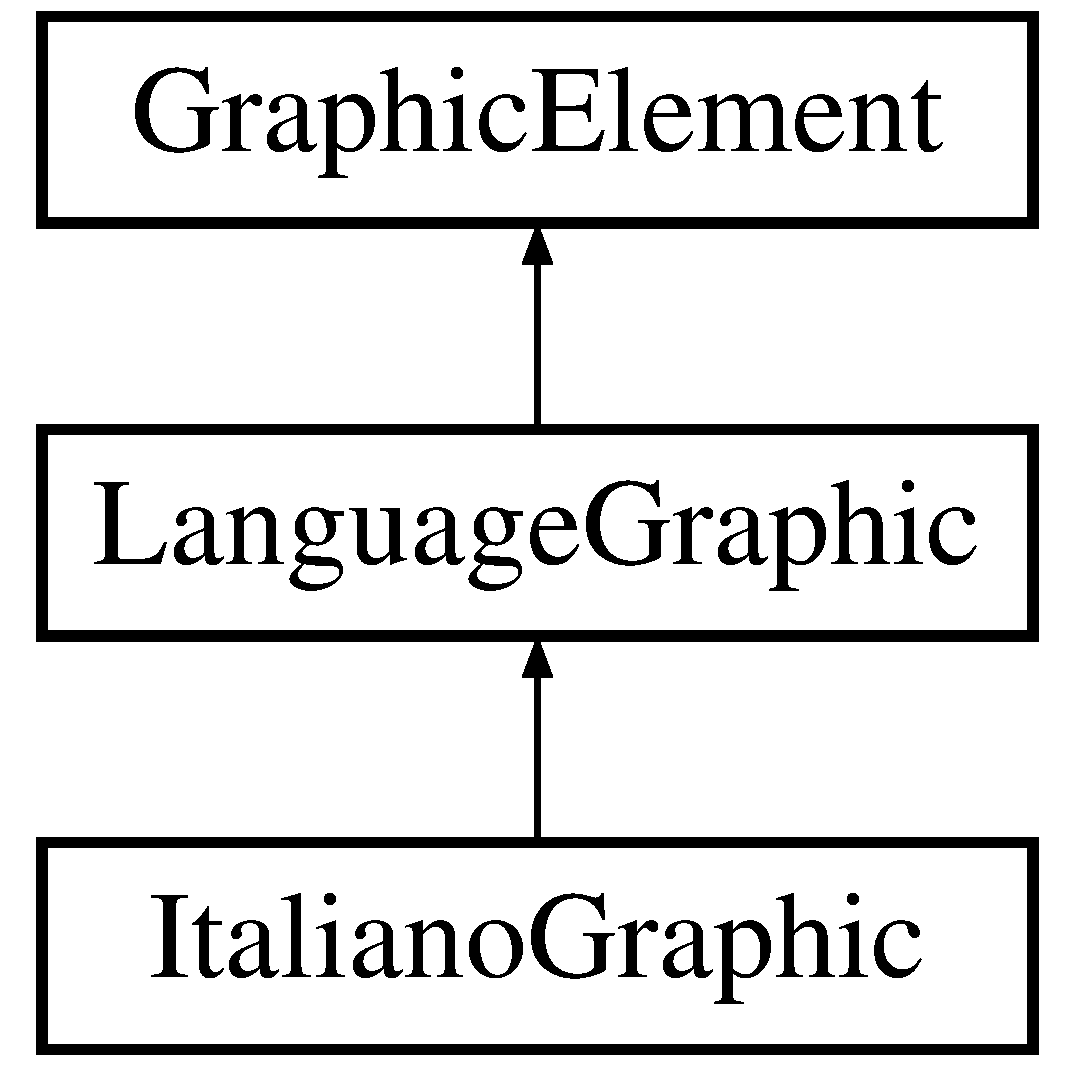
\includegraphics[height=3.000000cm]{class_italiano_graphic}
\end{center}
\end{figure}
\subsection*{Fonctions membres publiques}
\begin{DoxyCompactItemize}
\item 
\hypertarget{class_italiano_graphic_a04c213fd2d6388ec911aa0577f5d6846}{virtual void {\bfseries set\-Image\-To\-Sprite} ()}\label{class_italiano_graphic_a04c213fd2d6388ec911aa0577f5d6846}

\end{DoxyCompactItemize}
\subsection*{Membres hérités additionnels}


La documentation de cette classe a été générée à partir des fichiers suivants \-:\begin{DoxyCompactItemize}
\item 
/\-Users/\-Ananas/\-Desktop/\-Mes\-Projets\-Git/purupurudigger/\-Code\-Cpp/Italiano\-Graphic.\-h\item 
/\-Users/\-Ananas/\-Desktop/\-Mes\-Projets\-Git/purupurudigger/\-Code\-Cpp/Italiano\-Graphic.\-cpp\end{DoxyCompactItemize}

\hypertarget{class_language_graphic}{\section{Référence de la classe Language\-Graphic}
\label{class_language_graphic}\index{Language\-Graphic@{Language\-Graphic}}
}
Graphe d'héritage de Language\-Graphic\-:\begin{figure}[H]
\begin{center}
\leavevmode
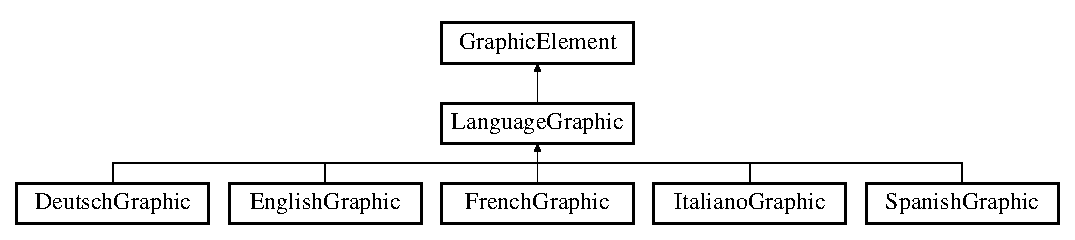
\includegraphics[height=2.776860cm]{class_language_graphic}
\end{center}
\end{figure}
\subsection*{Fonctions membres publiques}
\begin{DoxyCompactItemize}
\item 
\hypertarget{class_language_graphic_af84e2a15f4ffff39b23ae9f271530e10}{virtual void {\bfseries set\-Image\-To\-Sprite} ()}\label{class_language_graphic_af84e2a15f4ffff39b23ae9f271530e10}

\item 
\hypertarget{class_language_graphic_a5d97e74fa17437b7e506afaafdbd037a}{virtual void {\bfseries set\-Teacher\-Mode} ()}\label{class_language_graphic_a5d97e74fa17437b7e506afaafdbd037a}

\item 
\hypertarget{class_language_graphic_a452acee7fc2e289a30913b622ae29965}{virtual void {\bfseries set\-Ananas\-Mode} ()}\label{class_language_graphic_a452acee7fc2e289a30913b622ae29965}

\item 
\hypertarget{class_language_graphic_ab5c752f8c3d223e2a456521f96c86d79}{void {\bfseries set\-Hover} ()}\label{class_language_graphic_ab5c752f8c3d223e2a456521f96c86d79}

\item 
\hypertarget{class_language_graphic_acca816079c11a5cdb1d3b4aeb44a5d46}{void {\bfseries reset} ()}\label{class_language_graphic_acca816079c11a5cdb1d3b4aeb44a5d46}

\end{DoxyCompactItemize}
\subsection*{Attributs protégés statiques}
\begin{DoxyCompactItemize}
\item 
\hypertarget{class_language_graphic_a54664ca1c39562c8e506ba7873d6ad05}{static sf\-::\-Image {\bfseries my\-\_\-image}}\label{class_language_graphic_a54664ca1c39562c8e506ba7873d6ad05}

\end{DoxyCompactItemize}
\subsection*{Membres hérités additionnels}


La documentation de cette classe a été générée à partir des fichiers suivants \-:\begin{DoxyCompactItemize}
\item 
/\-Users/\-Ananas/\-Desktop/\-Mes\-Projets\-Git/purupurudigger/\-Code\-Cpp/Language\-Graphic.\-h\item 
/\-Users/\-Ananas/\-Desktop/\-Mes\-Projets\-Git/purupurudigger/\-Code\-Cpp/Language\-Graphic.\-cpp\end{DoxyCompactItemize}

\hypertarget{class_language_message}{\section{Référence de la classe Language\-Message}
\label{class_language_message}\index{Language\-Message@{Language\-Message}}
}


Classe pour enregistrer notre multilangue.  




{\ttfamily \#include $<$Language\-Message.\-h$>$}

\subsection*{Fonctions membres publiques}
\begin{DoxyCompactItemize}
\item 
\hyperlink{class_language_message_aed1448b1bcddacd0aa85ddeff0af8451}{Language\-Message} ()
\begin{DoxyCompactList}\small\item\em Constructeur. \end{DoxyCompactList}\item 
\hypertarget{class_language_message_a13dfa70f541da1eb2cd6eb3ea2aefc6f}{std\-::map$<$ \hyperlink{_constantes_8h_a4f09127c805cc1f5ee20e67db7b45efa}{Message}, std\-::string $>$ \& \hyperlink{class_language_message_a13dfa70f541da1eb2cd6eb3ea2aefc6f}{operator\mbox{[}$\,$\mbox{]}} (\hyperlink{_constantes_8h_a315ca917ad583797f709ea477dd28705}{Language} language)}\label{class_language_message_a13dfa70f541da1eb2cd6eb3ea2aefc6f}

\begin{DoxyCompactList}\small\item\em Surcharge de l'opérateur crochet. \end{DoxyCompactList}\end{DoxyCompactItemize}
\subsection*{Attributs publics}
\begin{DoxyCompactItemize}
\item 
std\-::map$<$ \hyperlink{_constantes_8h_a315ca917ad583797f709ea477dd28705}{Language}, std\-::map\\*
$<$ \hyperlink{_constantes_8h_a4f09127c805cc1f5ee20e67db7b45efa}{Message}, std\-::string $>$ $>$ \hyperlink{class_language_message_aed19151194189a85d29c9a2bbd4ff002}{my\-\_\-languages}
\end{DoxyCompactItemize}


\subsection{Description détaillée}
Classe pour enregistrer notre multilangue. 

\subsection{Documentation des constructeurs et destructeur}
\hypertarget{class_language_message_aed1448b1bcddacd0aa85ddeff0af8451}{\index{Language\-Message@{Language\-Message}!Language\-Message@{Language\-Message}}
\index{Language\-Message@{Language\-Message}!LanguageMessage@{Language\-Message}}
\subsubsection[{Language\-Message}]{\setlength{\rightskip}{0pt plus 5cm}Language\-Message\-::\-Language\-Message (
\begin{DoxyParamCaption}
{}
\end{DoxyParamCaption}
)}}\label{class_language_message_aed1448b1bcddacd0aa85ddeff0af8451}


Constructeur. 

Constructeur de la classe \hyperlink{class_language_message}{Language\-Message} 

\subsection{Documentation des données membres}
\hypertarget{class_language_message_aed19151194189a85d29c9a2bbd4ff002}{\index{Language\-Message@{Language\-Message}!my\-\_\-languages@{my\-\_\-languages}}
\index{my\-\_\-languages@{my\-\_\-languages}!LanguageMessage@{Language\-Message}}
\subsubsection[{my\-\_\-languages}]{\setlength{\rightskip}{0pt plus 5cm}std\-::map$<$ {\bf Language}, std\-::map$<$ {\bf Message}, std\-::string$>$ $>$ Language\-Message\-::my\-\_\-languages}}\label{class_language_message_aed19151194189a85d29c9a2bbd4ff002}
Notre map 

La documentation de cette classe a été générée à partir des fichiers suivants \-:\begin{DoxyCompactItemize}
\item 
/\-Users/\-Ananas/\-Desktop/\-Mes\-Projets\-Git/purupurudigger/\-Code\-Cpp/\hyperlink{_language_message_8h}{Language\-Message.\-h}\item 
/\-Users/\-Ananas/\-Desktop/\-Mes\-Projets\-Git/purupurudigger/\-Code\-Cpp/\hyperlink{_language_message_8cpp}{Language\-Message.\-cpp}\end{DoxyCompactItemize}

\hypertarget{class_level}{\section{Référence de la classe Level}
\label{class_level}\index{Level@{Level}}
}


Classe modélisant un level.  




{\ttfamily \#include $<$Level.\-h$>$}

\subsection*{Fonctions membres publiques}
\begin{DoxyCompactItemize}
\item 
\hypertarget{class_level_aca6522d3c16432468659428c2be31af2}{void \hyperlink{class_level_aca6522d3c16432468659428c2be31af2}{reset} ()}\label{class_level_aca6522d3c16432468659428c2be31af2}

\begin{DoxyCompactList}\small\item\em Méthode pour regénerer une grille après avoir perdu ou gagné sans perdre les attributs de notre \hyperlink{class_digger}{Digger}. \end{DoxyCompactList}\item 
\hyperlink{class_level_a40ebd1dfbcdd2ed15b7f9dfb98151df4}{Level} (\hyperlink{class_score}{Score} $\ast$score)
\begin{DoxyCompactList}\small\item\em Constructeur. \end{DoxyCompactList}\item 
\hyperlink{class_level_a249eac1e8f19ff44134efa5e986feaca}{$\sim$\-Level} ()
\begin{DoxyCompactList}\small\item\em Destructeur. \end{DoxyCompactList}\item 
void \hyperlink{class_level_a9291559602f5fb2cad18728b98a5f3fb}{lost\-Level} ()
\begin{DoxyCompactList}\small\item\em Perdre le level. \end{DoxyCompactList}\item 
void \hyperlink{class_level_a534a7bc704bb07bd9141fa9f6a869e50}{reset\-Win} ()
\begin{DoxyCompactList}\small\item\em remettre win a false \end{DoxyCompactList}\item 
void \hyperlink{class_level_ad56c1bf009f384ba4e721ff3d1691856}{reset\-Lose} ()
\begin{DoxyCompactList}\small\item\em remettre lose a false \end{DoxyCompactList}\item 
int \hyperlink{class_level_afa4a755701365c8f7e8f9e19286c8478}{get\-Goal} () const 
\begin{DoxyCompactList}\small\item\em Connaître l'objectif en point du \hyperlink{class_level}{Level}. \end{DoxyCompactList}\item 
int \hyperlink{class_level_ac3ae10185fc3529283360e8e038525d7}{get\-Current\-Move} () const 
\begin{DoxyCompactList}\small\item\em Connaître nos déplacements en cours. \end{DoxyCompactList}\item 
bool \hyperlink{class_level_a72494b188b4e0ad5e903dc87661d052f}{time\-Is\-Up} () const 
\begin{DoxyCompactList}\small\item\em Connaître si le temps est écoulé \end{DoxyCompactList}\item 
float \hyperlink{class_level_a8905da43f541f853f45224ea08cdc8ab}{left\-Time} () const 
\begin{DoxyCompactList}\small\item\em Connaître le temps restant. \end{DoxyCompactList}\item 
\hypertarget{class_level_a71db09429d1295bb6bc7d55ae4e5da25}{void \hyperlink{class_level_a71db09429d1295bb6bc7d55ae4e5da25}{reset\-Time} ()}\label{class_level_a71db09429d1295bb6bc7d55ae4e5da25}

\begin{DoxyCompactList}\small\item\em Connaître le temps actuelle à jour. \end{DoxyCompactList}\item 
\hyperlink{class_digger}{Digger} $\ast$const \hyperlink{class_level_a2c53239c70b357a0a2287762e06c9182}{get\-Digger} () const 
\begin{DoxyCompactList}\small\item\em Retourner notre digger pour avoir des informations sur lui. \end{DoxyCompactList}\item 
bool \hyperlink{class_level_a8b98e1d55d50e4d8d9cba54e96b72677}{is\-Cell\-Clickable} (int click\-\_\-x, int click\-\_\-y) const 
\begin{DoxyCompactList}\small\item\em Connaître si la case est franchissable ( de type numérique et à côté du \hyperlink{class_digger}{Digger}. \end{DoxyCompactList}\item 
const \hyperlink{_level_8h_aa52f3da1e4a1cd4aecda50840fed14ff}{Grid} \& \hyperlink{class_level_a777499d0a75fde6c16507539554d47ef}{get\-Grid} () const 
\begin{DoxyCompactList}\small\item\em Renvoyer notre grille ( affichage ) \end{DoxyCompactList}\item 
bool \hyperlink{class_level_a77f7a589835b97308725fb33cce9b180}{is\-Dead} () const 
\begin{DoxyCompactList}\small\item\em Connaître si notre \hyperlink{class_digger}{Digger} est définitivement mort. \end{DoxyCompactList}\item 
bool \hyperlink{class_level_a0a925be843eb5104640f6620fc1d60de}{win} () const 
\begin{DoxyCompactList}\small\item\em Connaître si l'on vient juste de gagner un niveau ( affichage ) \end{DoxyCompactList}\item 
bool \hyperlink{class_level_a0407f9f93fcc7f4b62243f19a08a151d}{lose} () const 
\begin{DoxyCompactList}\small\item\em Connaître si l'on vient juste de perdre un niveau ( affichage ) \end{DoxyCompactList}\item 
void \hyperlink{class_level_a856f5d48686f4ed8cb39c0c9bee65bda}{move\-West} ()
\begin{DoxyCompactList}\small\item\em Sucre pour se déplacer à gauche ( delta\-X 0, delta\-Y -\/1, voir la methode move() \end{DoxyCompactList}\item 
void \hyperlink{class_level_acfe6e8be0de8e13f4cbad5f21ed85228}{move\-East} ()
\begin{DoxyCompactList}\small\item\em Sucre pour se déplacer à droite ( delta\-X 0, delta\-Y 1, voir la methode move() \end{DoxyCompactList}\item 
void \hyperlink{class_level_ab9e3b417fd1f1c729d806b4cfbd3a818}{move\-North} ()
\begin{DoxyCompactList}\small\item\em Sucre pour se déplacer en haut ( delta\-X -\/1, delta\-Y 0, voir la methode move() \end{DoxyCompactList}\item 
void \hyperlink{class_level_a582ad2bd2ba5ac4b2caa878b28acd768}{move\-South} ()
\begin{DoxyCompactList}\small\item\em Sucre pour se déplacer en bas ( delta\-X 1, delta\-Y 0, voir la methode move() \end{DoxyCompactList}\item 
void \hyperlink{class_level_a3a1751a147b9c508123e4e7f2838fb65}{move\-North\-East} ()
\begin{DoxyCompactList}\small\item\em Sucre pour se déplacer en haut à droite ( delta\-X -\/1, delta\-Y 1, voir la methode move() \end{DoxyCompactList}\item 
void \hyperlink{class_level_a93288849fa5c50b2ccc95ea72824e426}{move\-North\-West} ()
\begin{DoxyCompactList}\small\item\em Sucre pour se déplacer en haut à gauche ( delta\-X -\/1, delta\-Y -\/1, voir la methode move() \end{DoxyCompactList}\item 
void \hyperlink{class_level_a4495effa976a4fd91fac4fce196bf34f}{move\-South\-West} ()
\begin{DoxyCompactList}\small\item\em Sucre pour se déplacer en bas à gauche ( delta\-X 1, delta\-Y -\/1, voir la methode move() \end{DoxyCompactList}\item 
void \hyperlink{class_level_a28aeb93c2ff6d17d313da1d3f621e0ad}{move\-South\-East} ()
\begin{DoxyCompactList}\small\item\em Sucre pour se déplacer en bas à droite ( delta\-X 1, delta\-Y 1, voir la methode move() \end{DoxyCompactList}\end{DoxyCompactItemize}


\subsection{Description détaillée}
Classe modélisant un level. 

\subsection{Documentation des constructeurs et destructeur}
\hypertarget{class_level_a40ebd1dfbcdd2ed15b7f9dfb98151df4}{\index{Level@{Level}!Level@{Level}}
\index{Level@{Level}!Level@{Level}}
\subsubsection[{Level}]{\setlength{\rightskip}{0pt plus 5cm}Level\-::\-Level (
\begin{DoxyParamCaption}
\item[{{\bf Score} $\ast$}]{score}
\end{DoxyParamCaption}
)}}\label{class_level_a40ebd1dfbcdd2ed15b7f9dfb98151df4}


Constructeur. 

Constructeur de la classe \hyperlink{class_level}{Level}


\begin{DoxyParams}{Paramètres}
{\em $\ast$score} & \-: score de notre partie (injection de dépendance ) \\
\hline
\end{DoxyParams}
\hypertarget{class_level_a249eac1e8f19ff44134efa5e986feaca}{\index{Level@{Level}!$\sim$\-Level@{$\sim$\-Level}}
\index{$\sim$\-Level@{$\sim$\-Level}!Level@{Level}}
\subsubsection[{$\sim$\-Level}]{\setlength{\rightskip}{0pt plus 5cm}Level\-::$\sim$\-Level (
\begin{DoxyParamCaption}
{}
\end{DoxyParamCaption}
)}}\label{class_level_a249eac1e8f19ff44134efa5e986feaca}


Destructeur. 

Destructeur de la classe \hyperlink{class_level}{Level} 

\subsection{Documentation des fonctions membres}
\hypertarget{class_level_ac3ae10185fc3529283360e8e038525d7}{\index{Level@{Level}!get\-Current\-Move@{get\-Current\-Move}}
\index{get\-Current\-Move@{get\-Current\-Move}!Level@{Level}}
\subsubsection[{get\-Current\-Move}]{\setlength{\rightskip}{0pt plus 5cm}int Level\-::get\-Current\-Move (
\begin{DoxyParamCaption}
{}
\end{DoxyParamCaption}
) const}}\label{class_level_ac3ae10185fc3529283360e8e038525d7}


Connaître nos déplacements en cours. 

\begin{DoxyReturn}{Renvoie}
my\-\_\-current\-Move 
\end{DoxyReturn}
\hypertarget{class_level_a2c53239c70b357a0a2287762e06c9182}{\index{Level@{Level}!get\-Digger@{get\-Digger}}
\index{get\-Digger@{get\-Digger}!Level@{Level}}
\subsubsection[{get\-Digger}]{\setlength{\rightskip}{0pt plus 5cm}{\bf Digger} $\ast$const Level\-::get\-Digger (
\begin{DoxyParamCaption}
{}
\end{DoxyParamCaption}
) const}}\label{class_level_a2c53239c70b357a0a2287762e06c9182}


Retourner notre digger pour avoir des informations sur lui. 

\begin{DoxyReturn}{Renvoie}
un pointeur sur notre digger 
\end{DoxyReturn}
\hypertarget{class_level_afa4a755701365c8f7e8f9e19286c8478}{\index{Level@{Level}!get\-Goal@{get\-Goal}}
\index{get\-Goal@{get\-Goal}!Level@{Level}}
\subsubsection[{get\-Goal}]{\setlength{\rightskip}{0pt plus 5cm}int Level\-::get\-Goal (
\begin{DoxyParamCaption}
{}
\end{DoxyParamCaption}
) const}}\label{class_level_afa4a755701365c8f7e8f9e19286c8478}


Connaître l'objectif en point du \hyperlink{class_level}{Level}. 

\begin{DoxyReturn}{Renvoie}
my\-\_\-goal 
\end{DoxyReturn}
\hypertarget{class_level_a777499d0a75fde6c16507539554d47ef}{\index{Level@{Level}!get\-Grid@{get\-Grid}}
\index{get\-Grid@{get\-Grid}!Level@{Level}}
\subsubsection[{get\-Grid}]{\setlength{\rightskip}{0pt plus 5cm}const {\bf Grid} \& Level\-::get\-Grid (
\begin{DoxyParamCaption}
{}
\end{DoxyParamCaption}
) const}}\label{class_level_a777499d0a75fde6c16507539554d47ef}


Renvoyer notre grille ( affichage ) 

\begin{DoxyReturn}{Renvoie}
my\-\_\-grid 
\end{DoxyReturn}
\hypertarget{class_level_a8b98e1d55d50e4d8d9cba54e96b72677}{\index{Level@{Level}!is\-Cell\-Clickable@{is\-Cell\-Clickable}}
\index{is\-Cell\-Clickable@{is\-Cell\-Clickable}!Level@{Level}}
\subsubsection[{is\-Cell\-Clickable}]{\setlength{\rightskip}{0pt plus 5cm}bool Level\-::is\-Cell\-Clickable (
\begin{DoxyParamCaption}
\item[{int}]{click\-\_\-x, }
\item[{int}]{click\-\_\-y}
\end{DoxyParamCaption}
) const}}\label{class_level_a8b98e1d55d50e4d8d9cba54e96b72677}


Connaître si la case est franchissable ( de type numérique et à côté du \hyperlink{class_digger}{Digger}. 

param\mbox{[}in\mbox{]} click\-\_\-x \-: la position verticale de notre click param\mbox{[}in\mbox{]} click\-\_\-y \-: la position horizontale de notre click

\begin{DoxyReturn}{Renvoie}
true si la case est franchissable 
\end{DoxyReturn}
Il faut vérifier si l'on ne sort pas du tableau

Il faut d'abord vérifier que la case est juste à côté de notre digger

On vérifie son type \hypertarget{class_level_a77f7a589835b97308725fb33cce9b180}{\index{Level@{Level}!is\-Dead@{is\-Dead}}
\index{is\-Dead@{is\-Dead}!Level@{Level}}
\subsubsection[{is\-Dead}]{\setlength{\rightskip}{0pt plus 5cm}bool Level\-::is\-Dead (
\begin{DoxyParamCaption}
{}
\end{DoxyParamCaption}
) const}}\label{class_level_a77f7a589835b97308725fb33cce9b180}


Connaître si notre \hyperlink{class_digger}{Digger} est définitivement mort. 

\begin{DoxyReturn}{Renvoie}
true si il est mort 
\end{DoxyReturn}
\hypertarget{class_level_a8905da43f541f853f45224ea08cdc8ab}{\index{Level@{Level}!left\-Time@{left\-Time}}
\index{left\-Time@{left\-Time}!Level@{Level}}
\subsubsection[{left\-Time}]{\setlength{\rightskip}{0pt plus 5cm}float Level\-::left\-Time (
\begin{DoxyParamCaption}
{}
\end{DoxyParamCaption}
) const}}\label{class_level_a8905da43f541f853f45224ea08cdc8ab}


Connaître le temps restant. 

\begin{DoxyReturn}{Renvoie}
le temps restant 
\end{DoxyReturn}
\hypertarget{class_level_a0407f9f93fcc7f4b62243f19a08a151d}{\index{Level@{Level}!lose@{lose}}
\index{lose@{lose}!Level@{Level}}
\subsubsection[{lose}]{\setlength{\rightskip}{0pt plus 5cm}bool Level\-::lose (
\begin{DoxyParamCaption}
{}
\end{DoxyParamCaption}
) const}}\label{class_level_a0407f9f93fcc7f4b62243f19a08a151d}


Connaître si l'on vient juste de perdre un niveau ( affichage ) 

\begin{DoxyReturn}{Renvoie}
true si l'on vient de perdre un niveau 
\end{DoxyReturn}
\hypertarget{class_level_a9291559602f5fb2cad18728b98a5f3fb}{\index{Level@{Level}!lost\-Level@{lost\-Level}}
\index{lost\-Level@{lost\-Level}!Level@{Level}}
\subsubsection[{lost\-Level}]{\setlength{\rightskip}{0pt plus 5cm}void Level\-::lost\-Level (
\begin{DoxyParamCaption}
{}
\end{DoxyParamCaption}
)}}\label{class_level_a9291559602f5fb2cad18728b98a5f3fb}


Perdre le level. 

Faire perdre une vie et regénération d'un niveau \hypertarget{class_level_acfe6e8be0de8e13f4cbad5f21ed85228}{\index{Level@{Level}!move\-East@{move\-East}}
\index{move\-East@{move\-East}!Level@{Level}}
\subsubsection[{move\-East}]{\setlength{\rightskip}{0pt plus 5cm}void Level\-::move\-East (
\begin{DoxyParamCaption}
{}
\end{DoxyParamCaption}
)}}\label{class_level_acfe6e8be0de8e13f4cbad5f21ed85228}


Sucre pour se déplacer à droite ( delta\-X 0, delta\-Y 1, voir la methode move() 

\begin{DoxySeeAlso}{Voir également}
deplacement 
\end{DoxySeeAlso}
\hypertarget{class_level_ab9e3b417fd1f1c729d806b4cfbd3a818}{\index{Level@{Level}!move\-North@{move\-North}}
\index{move\-North@{move\-North}!Level@{Level}}
\subsubsection[{move\-North}]{\setlength{\rightskip}{0pt plus 5cm}void Level\-::move\-North (
\begin{DoxyParamCaption}
{}
\end{DoxyParamCaption}
)}}\label{class_level_ab9e3b417fd1f1c729d806b4cfbd3a818}


Sucre pour se déplacer en haut ( delta\-X -\/1, delta\-Y 0, voir la methode move() 

\begin{DoxySeeAlso}{Voir également}
deplacement 
\end{DoxySeeAlso}
\hypertarget{class_level_a3a1751a147b9c508123e4e7f2838fb65}{\index{Level@{Level}!move\-North\-East@{move\-North\-East}}
\index{move\-North\-East@{move\-North\-East}!Level@{Level}}
\subsubsection[{move\-North\-East}]{\setlength{\rightskip}{0pt plus 5cm}void Level\-::move\-North\-East (
\begin{DoxyParamCaption}
{}
\end{DoxyParamCaption}
)}}\label{class_level_a3a1751a147b9c508123e4e7f2838fb65}


Sucre pour se déplacer en haut à droite ( delta\-X -\/1, delta\-Y 1, voir la methode move() 

\begin{DoxySeeAlso}{Voir également}
deplacement 
\end{DoxySeeAlso}
\hypertarget{class_level_a93288849fa5c50b2ccc95ea72824e426}{\index{Level@{Level}!move\-North\-West@{move\-North\-West}}
\index{move\-North\-West@{move\-North\-West}!Level@{Level}}
\subsubsection[{move\-North\-West}]{\setlength{\rightskip}{0pt plus 5cm}void Level\-::move\-North\-West (
\begin{DoxyParamCaption}
{}
\end{DoxyParamCaption}
)}}\label{class_level_a93288849fa5c50b2ccc95ea72824e426}


Sucre pour se déplacer en haut à gauche ( delta\-X -\/1, delta\-Y -\/1, voir la methode move() 

\begin{DoxySeeAlso}{Voir également}
deplacement 
\end{DoxySeeAlso}
\hypertarget{class_level_a582ad2bd2ba5ac4b2caa878b28acd768}{\index{Level@{Level}!move\-South@{move\-South}}
\index{move\-South@{move\-South}!Level@{Level}}
\subsubsection[{move\-South}]{\setlength{\rightskip}{0pt plus 5cm}void Level\-::move\-South (
\begin{DoxyParamCaption}
{}
\end{DoxyParamCaption}
)}}\label{class_level_a582ad2bd2ba5ac4b2caa878b28acd768}


Sucre pour se déplacer en bas ( delta\-X 1, delta\-Y 0, voir la methode move() 

\begin{DoxySeeAlso}{Voir également}
deplacement 
\end{DoxySeeAlso}
\hypertarget{class_level_a28aeb93c2ff6d17d313da1d3f621e0ad}{\index{Level@{Level}!move\-South\-East@{move\-South\-East}}
\index{move\-South\-East@{move\-South\-East}!Level@{Level}}
\subsubsection[{move\-South\-East}]{\setlength{\rightskip}{0pt plus 5cm}void Level\-::move\-South\-East (
\begin{DoxyParamCaption}
{}
\end{DoxyParamCaption}
)}}\label{class_level_a28aeb93c2ff6d17d313da1d3f621e0ad}


Sucre pour se déplacer en bas à droite ( delta\-X 1, delta\-Y 1, voir la methode move() 

\begin{DoxySeeAlso}{Voir également}
deplacement 
\end{DoxySeeAlso}
\hypertarget{class_level_a4495effa976a4fd91fac4fce196bf34f}{\index{Level@{Level}!move\-South\-West@{move\-South\-West}}
\index{move\-South\-West@{move\-South\-West}!Level@{Level}}
\subsubsection[{move\-South\-West}]{\setlength{\rightskip}{0pt plus 5cm}void Level\-::move\-South\-West (
\begin{DoxyParamCaption}
{}
\end{DoxyParamCaption}
)}}\label{class_level_a4495effa976a4fd91fac4fce196bf34f}


Sucre pour se déplacer en bas à gauche ( delta\-X 1, delta\-Y -\/1, voir la methode move() 

\begin{DoxySeeAlso}{Voir également}
deplacement 
\end{DoxySeeAlso}
\hypertarget{class_level_a856f5d48686f4ed8cb39c0c9bee65bda}{\index{Level@{Level}!move\-West@{move\-West}}
\index{move\-West@{move\-West}!Level@{Level}}
\subsubsection[{move\-West}]{\setlength{\rightskip}{0pt plus 5cm}void Level\-::move\-West (
\begin{DoxyParamCaption}
{}
\end{DoxyParamCaption}
)}}\label{class_level_a856f5d48686f4ed8cb39c0c9bee65bda}


Sucre pour se déplacer à gauche ( delta\-X 0, delta\-Y -\/1, voir la methode move() 

\begin{DoxySeeAlso}{Voir également}
deplacement 
\end{DoxySeeAlso}
\hypertarget{class_level_ad56c1bf009f384ba4e721ff3d1691856}{\index{Level@{Level}!reset\-Lose@{reset\-Lose}}
\index{reset\-Lose@{reset\-Lose}!Level@{Level}}
\subsubsection[{reset\-Lose}]{\setlength{\rightskip}{0pt plus 5cm}void Level\-::reset\-Lose (
\begin{DoxyParamCaption}
{}
\end{DoxyParamCaption}
)}}\label{class_level_ad56c1bf009f384ba4e721ff3d1691856}


remettre lose a false 

remet l'attribut lose false \hypertarget{class_level_a534a7bc704bb07bd9141fa9f6a869e50}{\index{Level@{Level}!reset\-Win@{reset\-Win}}
\index{reset\-Win@{reset\-Win}!Level@{Level}}
\subsubsection[{reset\-Win}]{\setlength{\rightskip}{0pt plus 5cm}void Level\-::reset\-Win (
\begin{DoxyParamCaption}
{}
\end{DoxyParamCaption}
)}}\label{class_level_a534a7bc704bb07bd9141fa9f6a869e50}


remettre win a false 

remet l'attribut win false \hypertarget{class_level_a72494b188b4e0ad5e903dc87661d052f}{\index{Level@{Level}!time\-Is\-Up@{time\-Is\-Up}}
\index{time\-Is\-Up@{time\-Is\-Up}!Level@{Level}}
\subsubsection[{time\-Is\-Up}]{\setlength{\rightskip}{0pt plus 5cm}bool Level\-::time\-Is\-Up (
\begin{DoxyParamCaption}
{}
\end{DoxyParamCaption}
) const}}\label{class_level_a72494b188b4e0ad5e903dc87661d052f}


Connaître si le temps est écoulé 

\begin{DoxyReturn}{Renvoie}
true si le temps est écoulé 
\end{DoxyReturn}
\hypertarget{class_level_a0a925be843eb5104640f6620fc1d60de}{\index{Level@{Level}!win@{win}}
\index{win@{win}!Level@{Level}}
\subsubsection[{win}]{\setlength{\rightskip}{0pt plus 5cm}bool Level\-::win (
\begin{DoxyParamCaption}
{}
\end{DoxyParamCaption}
) const}}\label{class_level_a0a925be843eb5104640f6620fc1d60de}


Connaître si l'on vient juste de gagner un niveau ( affichage ) 

\begin{DoxyReturn}{Renvoie}
true si l'on vient de gagner un niveau 
\end{DoxyReturn}


La documentation de cette classe a été générée à partir des fichiers suivants \-:\begin{DoxyCompactItemize}
\item 
/\-Users/\-Ananas/\-Desktop/\-Mes\-Projets\-Git/purupurudigger/\-Code\-Cpp/\hyperlink{_level_8h}{Level.\-h}\item 
/\-Users/\-Ananas/\-Desktop/\-Mes\-Projets\-Git/purupurudigger/\-Code\-Cpp/\hyperlink{_level_8cpp}{Level.\-cpp}\end{DoxyCompactItemize}

\hypertarget{class_score}{\section{Référence de la classe Score}
\label{class_score}\index{Score@{Score}}
}


Classe modélisant un score.  




{\ttfamily \#include $<$Score.\-h$>$}

\subsection*{Fonctions membres publiques}
\begin{DoxyCompactItemize}
\item 
\hyperlink{class_score_a039c99843551e5e4b512ecee99e46617}{Score} ()
\begin{DoxyCompactList}\small\item\em Constructeur. \end{DoxyCompactList}\item 
int \hyperlink{class_score_afcc13cb223fd905475a59693921451f8}{get\-Current} () const 
\begin{DoxyCompactList}\small\item\em Connaître le score courant. \end{DoxyCompactList}\item 
int \hyperlink{class_score_a68f116f8c2e0b732ee89949b0a403767}{get\-Current\-Step} () const 
\begin{DoxyCompactList}\small\item\em Connaître le niveau. \end{DoxyCompactList}\item 
int \hyperlink{class_score_a74a8797f08b2bbaa5883ec9daa4235a1}{get\-Globale} () const 
\begin{DoxyCompactList}\small\item\em Connaître le score totale. \end{DoxyCompactList}\item 
\hypertarget{class_score_a5c9ffcdf9765a29eb2ddf0d6dec622f6}{void \hyperlink{class_score_a5c9ffcdf9765a29eb2ddf0d6dec622f6}{add\-Success} ()}\label{class_score_a5c9ffcdf9765a29eb2ddf0d6dec622f6}

\begin{DoxyCompactList}\small\item\em Ajoute une case à notre tableau. \end{DoxyCompactList}\item 
\hypertarget{class_score_ade936f4b478e9b5b5188e5232b6f1a0f}{void \hyperlink{class_score_ade936f4b478e9b5b5188e5232b6f1a0f}{reset\-Score} ()}\label{class_score_ade936f4b478e9b5b5188e5232b6f1a0f}

\begin{DoxyCompactList}\small\item\em Remet à 0 la valeur de la dernière case de notre tableau. \end{DoxyCompactList}\item 
void \hyperlink{class_score_a5be24d8d1d1de90eaa68fec905b59ee6}{add\-Points} (const int \&i)
\begin{DoxyCompactList}\small\item\em Ajoute des points à notre case courante. \end{DoxyCompactList}\end{DoxyCompactItemize}


\subsection{Description détaillée}
Classe modélisant un score. 

\subsection{Documentation des constructeurs et destructeur}
\hypertarget{class_score_a039c99843551e5e4b512ecee99e46617}{\index{Score@{Score}!Score@{Score}}
\index{Score@{Score}!Score@{Score}}
\subsubsection[{Score}]{\setlength{\rightskip}{0pt plus 5cm}Score\-::\-Score (
\begin{DoxyParamCaption}
{}
\end{DoxyParamCaption}
)}}\label{class_score_a039c99843551e5e4b512ecee99e46617}


Constructeur. 

Constructeur de la classe \hyperlink{class_score}{Score} 

\subsection{Documentation des fonctions membres}
\hypertarget{class_score_a5be24d8d1d1de90eaa68fec905b59ee6}{\index{Score@{Score}!add\-Points@{add\-Points}}
\index{add\-Points@{add\-Points}!Score@{Score}}
\subsubsection[{add\-Points}]{\setlength{\rightskip}{0pt plus 5cm}void Score\-::add\-Points (
\begin{DoxyParamCaption}
\item[{const int \&}]{i}
\end{DoxyParamCaption}
)}}\label{class_score_a5be24d8d1d1de90eaa68fec905b59ee6}


Ajoute des points à notre case courante. 


\begin{DoxyParams}[1]{Paramètres}
\mbox{\tt in}  & {\em la} & valeur de ce que l'on doit ajouter à notre score courant \\
\hline
\end{DoxyParams}
\hypertarget{class_score_afcc13cb223fd905475a59693921451f8}{\index{Score@{Score}!get\-Current@{get\-Current}}
\index{get\-Current@{get\-Current}!Score@{Score}}
\subsubsection[{get\-Current}]{\setlength{\rightskip}{0pt plus 5cm}int Score\-::get\-Current (
\begin{DoxyParamCaption}
{}
\end{DoxyParamCaption}
) const}}\label{class_score_afcc13cb223fd905475a59693921451f8}


Connaître le score courant. 

\begin{DoxyReturn}{Renvoie}
la valeur de la dernière case de notre tableau de score 
\end{DoxyReturn}
\hypertarget{class_score_a68f116f8c2e0b732ee89949b0a403767}{\index{Score@{Score}!get\-Current\-Step@{get\-Current\-Step}}
\index{get\-Current\-Step@{get\-Current\-Step}!Score@{Score}}
\subsubsection[{get\-Current\-Step}]{\setlength{\rightskip}{0pt plus 5cm}int Score\-::get\-Current\-Step (
\begin{DoxyParamCaption}
{}
\end{DoxyParamCaption}
) const}}\label{class_score_a68f116f8c2e0b732ee89949b0a403767}


Connaître le niveau. 

\begin{DoxyReturn}{Renvoie}
la taille de notre tableau de score 
\end{DoxyReturn}
\hypertarget{class_score_a74a8797f08b2bbaa5883ec9daa4235a1}{\index{Score@{Score}!get\-Globale@{get\-Globale}}
\index{get\-Globale@{get\-Globale}!Score@{Score}}
\subsubsection[{get\-Globale}]{\setlength{\rightskip}{0pt plus 5cm}int Score\-::get\-Globale (
\begin{DoxyParamCaption}
{}
\end{DoxyParamCaption}
) const}}\label{class_score_a74a8797f08b2bbaa5883ec9daa4235a1}


Connaître le score totale. 

\begin{DoxyReturn}{Renvoie}
la somme du contenu de notre tableau de score 
\end{DoxyReturn}


La documentation de cette classe a été générée à partir des fichiers suivants \-:\begin{DoxyCompactItemize}
\item 
/\-Users/\-Ananas/\-Desktop/\-Mes\-Projets\-Git/purupurudigger/\-Code\-Cpp/\hyperlink{_score_8h}{Score.\-h}\item 
/\-Users/\-Ananas/\-Desktop/\-Mes\-Projets\-Git/purupurudigger/\-Code\-Cpp/\hyperlink{_score_8cpp}{Score.\-cpp}\end{DoxyCompactItemize}

\hypertarget{class_spanish_graphic}{\section{Référence de la classe Spanish\-Graphic}
\label{class_spanish_graphic}\index{Spanish\-Graphic@{Spanish\-Graphic}}
}
Graphe d'héritage de Spanish\-Graphic\-:\begin{figure}[H]
\begin{center}
\leavevmode
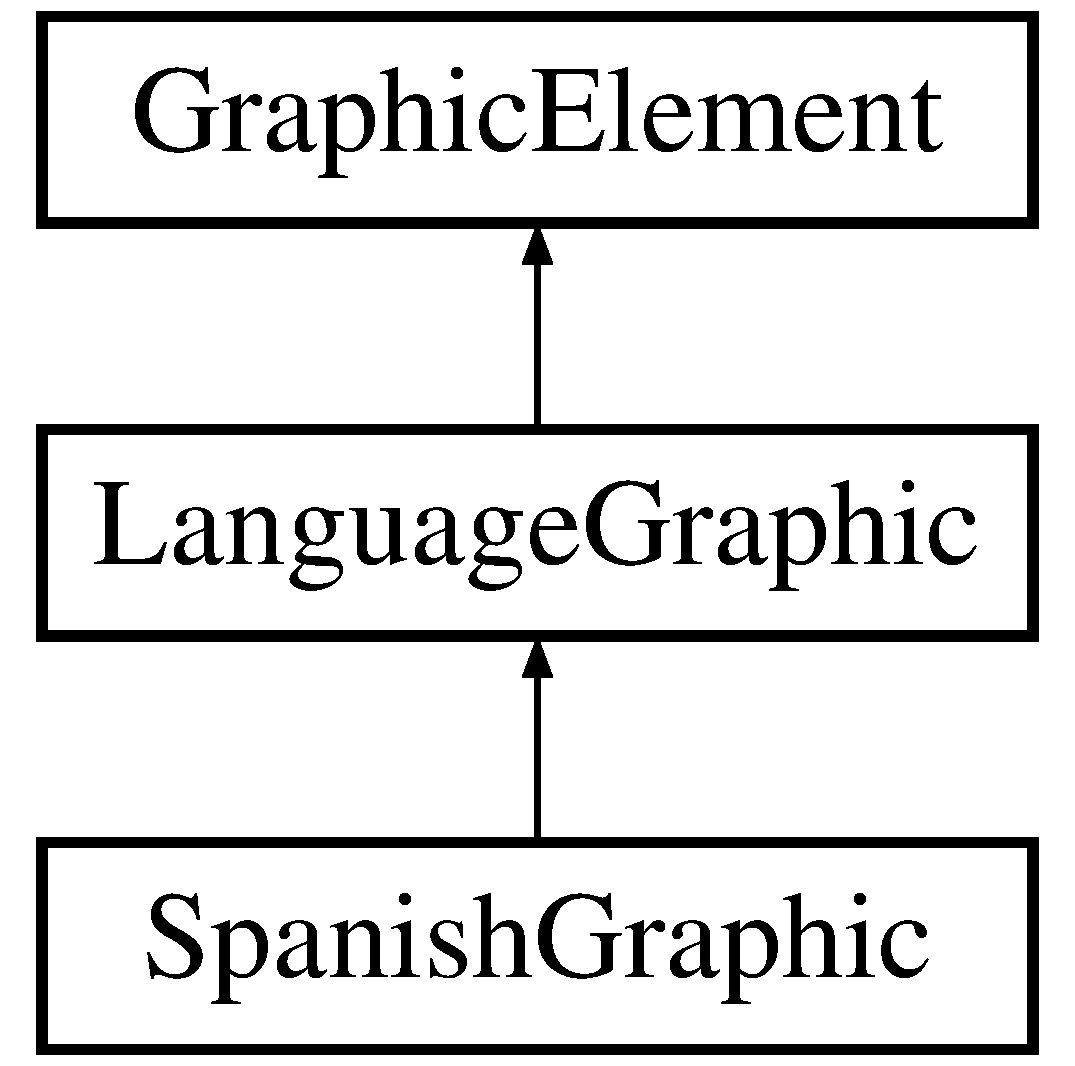
\includegraphics[height=3.000000cm]{class_spanish_graphic}
\end{center}
\end{figure}
\subsection*{Fonctions membres publiques}
\begin{DoxyCompactItemize}
\item 
\hypertarget{class_spanish_graphic_a7489943639278c9586612319afea18fa}{virtual void {\bfseries set\-Image\-To\-Sprite} ()}\label{class_spanish_graphic_a7489943639278c9586612319afea18fa}

\end{DoxyCompactItemize}
\subsection*{Membres hérités additionnels}


La documentation de cette classe a été générée à partir des fichiers suivants \-:\begin{DoxyCompactItemize}
\item 
/\-Users/\-Ananas/\-Desktop/\-Mes\-Projets\-Git/purupurudigger/\-Code\-Cpp/Spanish\-Graphic.\-h\item 
/\-Users/\-Ananas/\-Desktop/\-Mes\-Projets\-Git/purupurudigger/\-Code\-Cpp/Spanish\-Graphic.\-cpp\end{DoxyCompactItemize}

\hypertarget{class_sprite_graphic}{\section{Référence de la classe Sprite\-Graphic}
\label{class_sprite_graphic}\index{Sprite\-Graphic@{Sprite\-Graphic}}
}
Graphe d'héritage de Sprite\-Graphic\-:\begin{figure}[H]
\begin{center}
\leavevmode
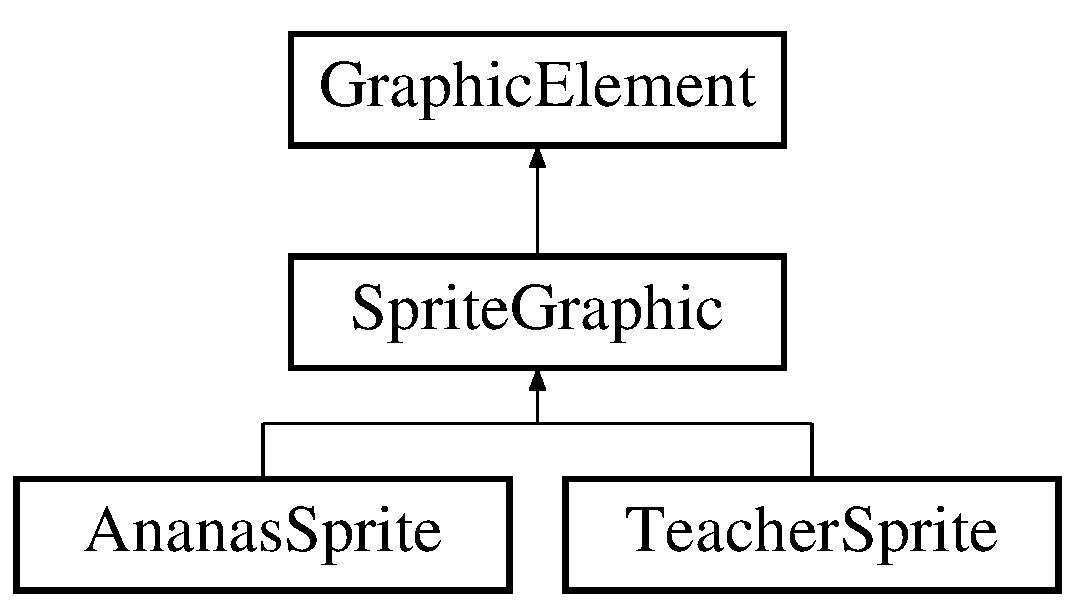
\includegraphics[height=3.000000cm]{class_sprite_graphic}
\end{center}
\end{figure}
\subsection*{Fonctions membres publiques}
\begin{DoxyCompactItemize}
\item 
\hypertarget{class_sprite_graphic_a4a559dacce663979705382433fca8c5a}{virtual void {\bfseries set\-Image\-To\-Sprite} ()}\label{class_sprite_graphic_a4a559dacce663979705382433fca8c5a}

\item 
\hypertarget{class_sprite_graphic_af855afb67c7368f31708d8175741367a}{virtual void {\bfseries set\-Teacher\-Mode} ()}\label{class_sprite_graphic_af855afb67c7368f31708d8175741367a}

\item 
\hypertarget{class_sprite_graphic_afae9b4e50c4787d6487bb9930989c225}{virtual void {\bfseries set\-Ananas\-Mode} ()}\label{class_sprite_graphic_afae9b4e50c4787d6487bb9930989c225}

\end{DoxyCompactItemize}
\subsection*{Attributs protégés statiques}
\begin{DoxyCompactItemize}
\item 
\hypertarget{class_sprite_graphic_a405a4e6f383dfd0c3a7c68c82ed35e5f}{static sf\-::\-Image {\bfseries my\-\_\-image}}\label{class_sprite_graphic_a405a4e6f383dfd0c3a7c68c82ed35e5f}

\end{DoxyCompactItemize}
\subsection*{Membres hérités additionnels}


La documentation de cette classe a été générée à partir des fichiers suivants \-:\begin{DoxyCompactItemize}
\item 
/\-Users/\-Ananas/\-Desktop/\-Mes\-Projets\-Git/purupurudigger/\-Code\-Cpp/Sprite\-Graphic.\-h\item 
/\-Users/\-Ananas/\-Desktop/\-Mes\-Projets\-Git/purupurudigger/\-Code\-Cpp/Sprite\-Graphic.\-cpp\end{DoxyCompactItemize}

\hypertarget{class_teacher_sprite}{\section{Référence de la classe Teacher\-Sprite}
\label{class_teacher_sprite}\index{Teacher\-Sprite@{Teacher\-Sprite}}
}
Graphe d'héritage de Teacher\-Sprite\-:\begin{figure}[H]
\begin{center}
\leavevmode
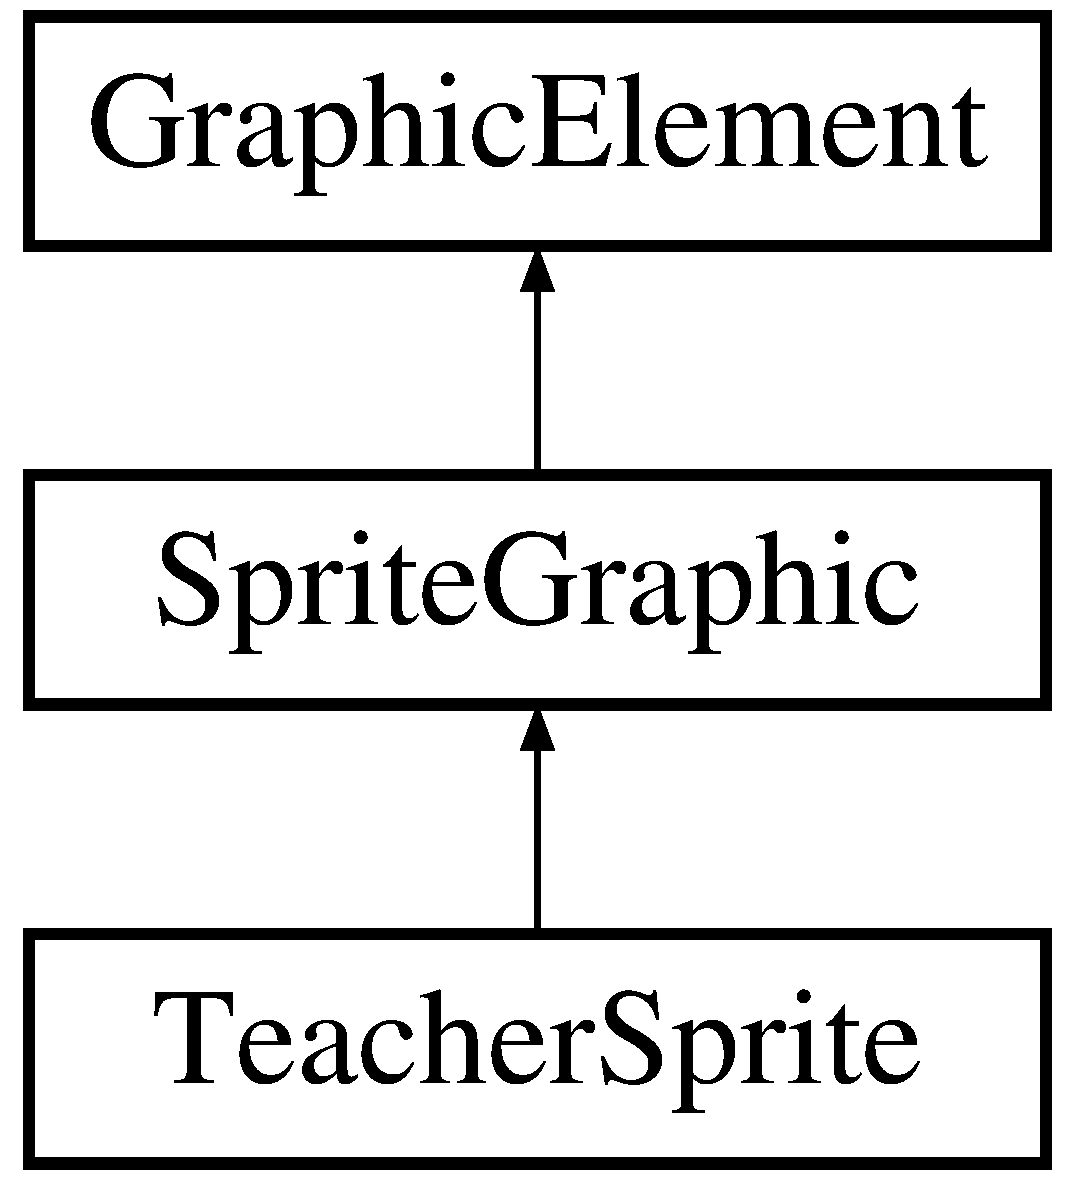
\includegraphics[height=3.000000cm]{class_teacher_sprite}
\end{center}
\end{figure}
\subsection*{Fonctions membres publiques}
\begin{DoxyCompactItemize}
\item 
\hypertarget{class_teacher_sprite_af27b172df663abe2bcfca26d7bf0f53c}{virtual void {\bfseries set\-Image\-To\-Sprite} ()}\label{class_teacher_sprite_af27b172df663abe2bcfca26d7bf0f53c}

\end{DoxyCompactItemize}
\subsection*{Membres hérités additionnels}


La documentation de cette classe a été générée à partir des fichiers suivants \-:\begin{DoxyCompactItemize}
\item 
/\-Users/\-Ananas/\-Desktop/\-Mes\-Projets\-Git/purupurudigger/\-Code\-Cpp/Teacher\-Sprite.\-h\item 
/\-Users/\-Ananas/\-Desktop/\-Mes\-Projets\-Git/purupurudigger/\-Code\-Cpp/Teacher\-Sprite.\-cpp\end{DoxyCompactItemize}

\hypertarget{class_value_cell}{\section{Référence de la classe Value\-Cell}
\label{class_value_cell}\index{Value\-Cell@{Value\-Cell}}
}


Classe modélisant ce qu'est une \hyperlink{class_value_cell}{Value\-Cell}.  




{\ttfamily \#include $<$Value\-Cell.\-h$>$}

Graphe d'héritage de Value\-Cell\-:\begin{figure}[H]
\begin{center}
\leavevmode
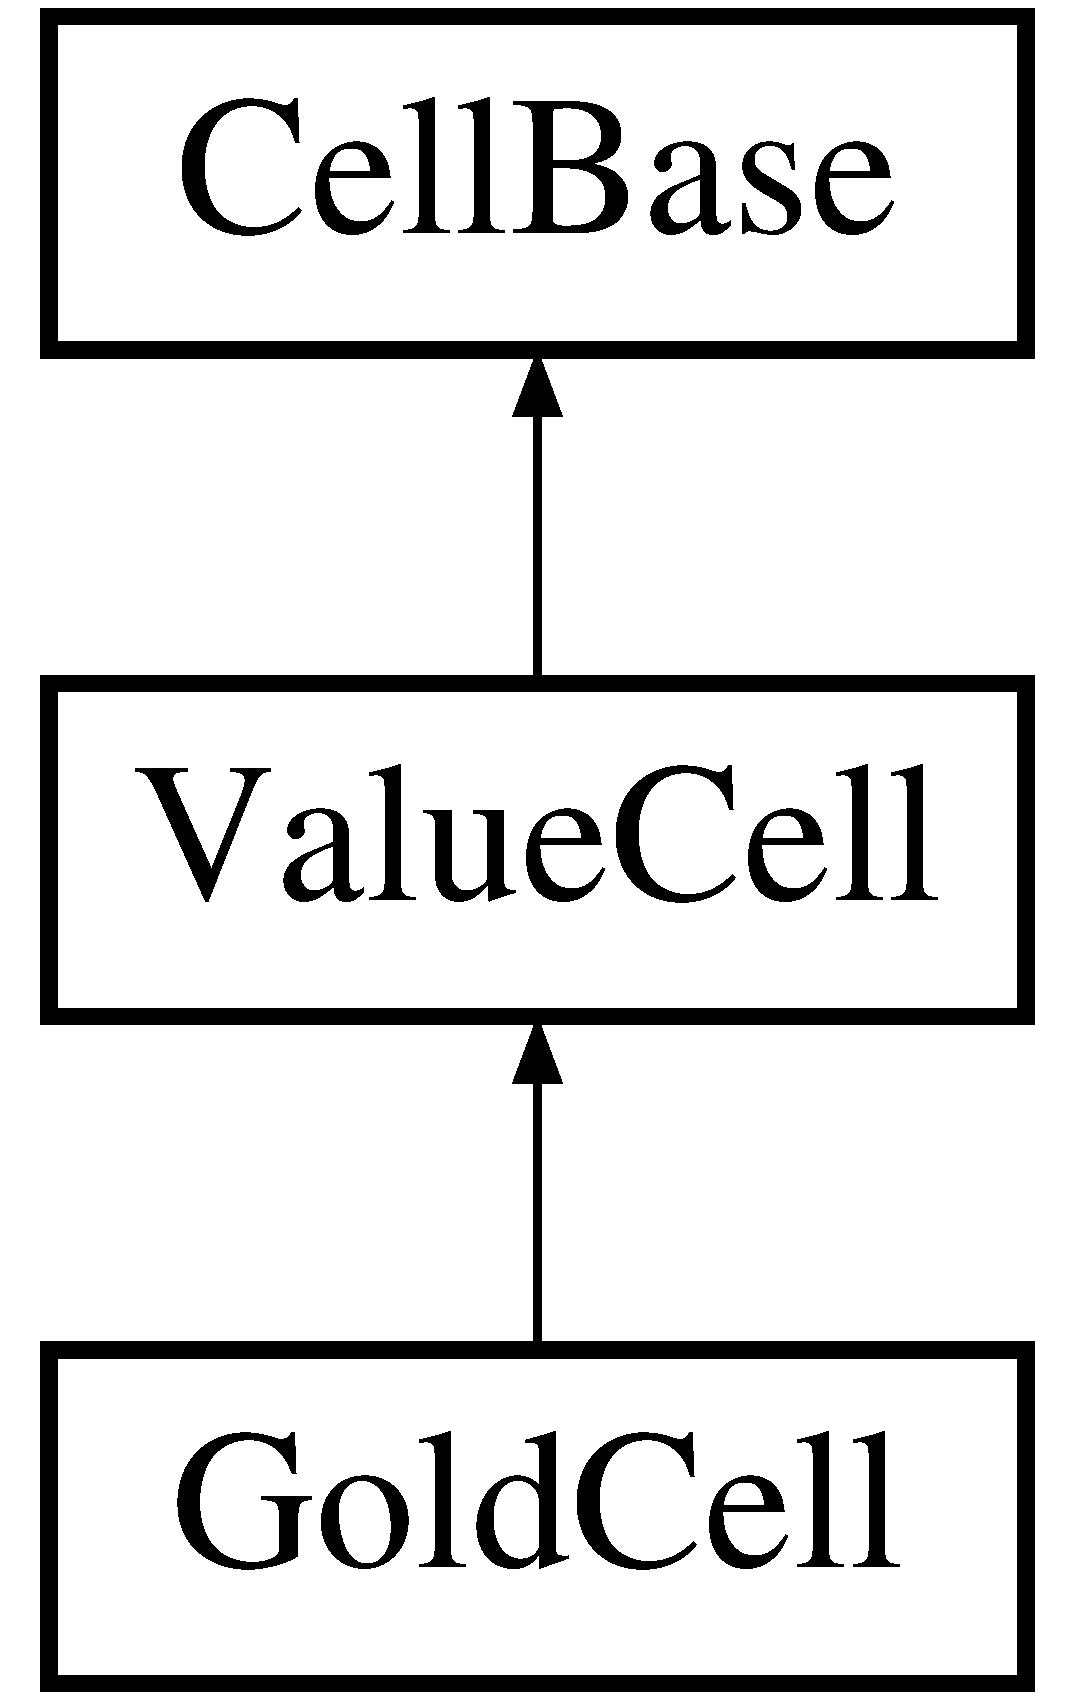
\includegraphics[height=3.000000cm]{class_value_cell}
\end{center}
\end{figure}
\subsection*{Fonctions membres publiques}
\begin{DoxyCompactItemize}
\item 
\hyperlink{class_value_cell_a396940ba9e81a9e379f3d55963f29a11}{Value\-Cell} ()
\begin{DoxyCompactList}\small\item\em Constructeur. \end{DoxyCompactList}\item 
\hyperlink{class_value_cell_af86c31417f0a2073b56f4e9fa3e4de32}{Value\-Cell} (int x, int y)
\begin{DoxyCompactList}\small\item\em Constructeur paramétré \end{DoxyCompactList}\item 
\hyperlink{class_value_cell_af45bf8b6d1678f18e47c305c7bc8d7f0}{Value\-Cell} (const \hyperlink{class_value_cell}{Value\-Cell} \&v)
\begin{DoxyCompactList}\small\item\em Constructeur par copie. \end{DoxyCompactList}\item 
virtual \hyperlink{class_value_cell_a5fae05f9343efe76a1cc8e91d2194d60}{$\sim$\-Value\-Cell} ()
\begin{DoxyCompactList}\small\item\em Destructeur. \end{DoxyCompactList}\item 
virtual int \hyperlink{class_value_cell_a8868208306d97f8f0a7b3b37119f6351}{get\-Value} () const 
\begin{DoxyCompactList}\small\item\em Retourne les points que va ajouter la case dans les scores. \end{DoxyCompactList}\item 
virtual int \hyperlink{class_value_cell_a711326876009350576251e512fcf126e}{get\-Points} () const 
\begin{DoxyCompactList}\small\item\em Retourne les points que va ajouter la case dans les scores. \end{DoxyCompactList}\item 
virtual \hyperlink{class_value_cell}{Value\-Cell} \& \hyperlink{class_value_cell_a321b5f779a6d72254b4dd419ee5f776e}{operator=} (const \hyperlink{class_value_cell}{Value\-Cell} \&v)
\begin{DoxyCompactList}\small\item\em Opérateur d'affectation pour recopier une \hyperlink{class_value_cell}{Value\-Cell}. \end{DoxyCompactList}\end{DoxyCompactItemize}
\subsection*{Fonctions membres protégées}
\begin{DoxyCompactItemize}
\item 
\hypertarget{class_value_cell_ae51fec7f6a31ee244a1d8eb063889e8f}{virtual void {\bfseries to\-Clone} (const \hyperlink{class_value_cell}{Value\-Cell} \&v)}\label{class_value_cell_ae51fec7f6a31ee244a1d8eb063889e8f}

\end{DoxyCompactItemize}
\subsection*{Attributs protégés}
\begin{DoxyCompactItemize}
\item 
int \hyperlink{class_value_cell_a630739966000f7611688a725bdea7d16}{my\-\_\-value}
\end{DoxyCompactItemize}


\subsection{Description détaillée}
Classe modélisant ce qu'est une \hyperlink{class_value_cell}{Value\-Cell}. 

\subsection{Documentation des constructeurs et destructeur}
\hypertarget{class_value_cell_a396940ba9e81a9e379f3d55963f29a11}{\index{Value\-Cell@{Value\-Cell}!Value\-Cell@{Value\-Cell}}
\index{Value\-Cell@{Value\-Cell}!ValueCell@{Value\-Cell}}
\subsubsection[{Value\-Cell}]{\setlength{\rightskip}{0pt plus 5cm}Value\-Cell\-::\-Value\-Cell (
\begin{DoxyParamCaption}
{}
\end{DoxyParamCaption}
)}}\label{class_value_cell_a396940ba9e81a9e379f3d55963f29a11}


Constructeur. 

Constructeur de la classe \hyperlink{class_value_cell}{Value\-Cell} \hypertarget{class_value_cell_af86c31417f0a2073b56f4e9fa3e4de32}{\index{Value\-Cell@{Value\-Cell}!Value\-Cell@{Value\-Cell}}
\index{Value\-Cell@{Value\-Cell}!ValueCell@{Value\-Cell}}
\subsubsection[{Value\-Cell}]{\setlength{\rightskip}{0pt plus 5cm}Value\-Cell\-::\-Value\-Cell (
\begin{DoxyParamCaption}
\item[{int}]{x, }
\item[{int}]{y}
\end{DoxyParamCaption}
)}}\label{class_value_cell_af86c31417f0a2073b56f4e9fa3e4de32}


Constructeur paramétré 

Constructeur paramétré de la classe \hyperlink{class_gold_cell}{Gold\-Cell} \hypertarget{class_value_cell_af45bf8b6d1678f18e47c305c7bc8d7f0}{\index{Value\-Cell@{Value\-Cell}!Value\-Cell@{Value\-Cell}}
\index{Value\-Cell@{Value\-Cell}!ValueCell@{Value\-Cell}}
\subsubsection[{Value\-Cell}]{\setlength{\rightskip}{0pt plus 5cm}Value\-Cell\-::\-Value\-Cell (
\begin{DoxyParamCaption}
\item[{const {\bf Value\-Cell} \&}]{v}
\end{DoxyParamCaption}
)}}\label{class_value_cell_af45bf8b6d1678f18e47c305c7bc8d7f0}


Constructeur par copie. 


\begin{DoxyParams}[1]{Paramètres}
\mbox{\tt in}  & {\em \hyperlink{class_value_cell}{Value\-Cell}} & v \\
\hline
\mbox{\tt out}  & {\em \hyperlink{class_value_cell}{Value\-Cell}} & v \\
\hline
\end{DoxyParams}
\hypertarget{class_value_cell_a5fae05f9343efe76a1cc8e91d2194d60}{\index{Value\-Cell@{Value\-Cell}!$\sim$\-Value\-Cell@{$\sim$\-Value\-Cell}}
\index{$\sim$\-Value\-Cell@{$\sim$\-Value\-Cell}!ValueCell@{Value\-Cell}}
\subsubsection[{$\sim$\-Value\-Cell}]{\setlength{\rightskip}{0pt plus 5cm}Value\-Cell\-::$\sim$\-Value\-Cell (
\begin{DoxyParamCaption}
{}
\end{DoxyParamCaption}
)\hspace{0.3cm}{\ttfamily [virtual]}}}\label{class_value_cell_a5fae05f9343efe76a1cc8e91d2194d60}


Destructeur. 

Destructeur de la classe fille \hyperlink{class_value_cell}{Value\-Cell} 

\subsection{Documentation des fonctions membres}
\hypertarget{class_value_cell_a711326876009350576251e512fcf126e}{\index{Value\-Cell@{Value\-Cell}!get\-Points@{get\-Points}}
\index{get\-Points@{get\-Points}!ValueCell@{Value\-Cell}}
\subsubsection[{get\-Points}]{\setlength{\rightskip}{0pt plus 5cm}int Value\-Cell\-::get\-Points (
\begin{DoxyParamCaption}
{}
\end{DoxyParamCaption}
) const\hspace{0.3cm}{\ttfamily [virtual]}}}\label{class_value_cell_a711326876009350576251e512fcf126e}


Retourne les points que va ajouter la case dans les scores. 

\begin{DoxyReturn}{Renvoie}
my\-\_\-points, retourne la valeur de la case 
\end{DoxyReturn}


Réimplémentée dans \hyperlink{class_gold_cell_a1f111db9bdb520176a48bb689c7baf2b}{Gold\-Cell}.

\hypertarget{class_value_cell_a8868208306d97f8f0a7b3b37119f6351}{\index{Value\-Cell@{Value\-Cell}!get\-Value@{get\-Value}}
\index{get\-Value@{get\-Value}!ValueCell@{Value\-Cell}}
\subsubsection[{get\-Value}]{\setlength{\rightskip}{0pt plus 5cm}int Value\-Cell\-::get\-Value (
\begin{DoxyParamCaption}
{}
\end{DoxyParamCaption}
) const\hspace{0.3cm}{\ttfamily [virtual]}}}\label{class_value_cell_a8868208306d97f8f0a7b3b37119f6351}


Retourne les points que va ajouter la case dans les scores. 

\begin{DoxyReturn}{Renvoie}
my\-\_\-value, retourne la valeur de la case 
\end{DoxyReturn}
\hypertarget{class_value_cell_a321b5f779a6d72254b4dd419ee5f776e}{\index{Value\-Cell@{Value\-Cell}!operator=@{operator=}}
\index{operator=@{operator=}!ValueCell@{Value\-Cell}}
\subsubsection[{operator=}]{\setlength{\rightskip}{0pt plus 5cm}{\bf Value\-Cell} \& Value\-Cell\-::operator= (
\begin{DoxyParamCaption}
\item[{const {\bf Value\-Cell} \&}]{v}
\end{DoxyParamCaption}
)\hspace{0.3cm}{\ttfamily [virtual]}}}\label{class_value_cell_a321b5f779a6d72254b4dd419ee5f776e}


Opérateur d'affectation pour recopier une \hyperlink{class_value_cell}{Value\-Cell}. 


\begin{DoxyParams}[1]{Paramètres}
\mbox{\tt in}  & {\em \hyperlink{class_value_cell}{Value\-Cell}} & v \-: opérateur d'affectation pour recopier une \hyperlink{class_gold_cell}{Gold\-Cell} \\
\hline
\end{DoxyParams}


\subsection{Documentation des données membres}
\hypertarget{class_value_cell_a630739966000f7611688a725bdea7d16}{\index{Value\-Cell@{Value\-Cell}!my\-\_\-value@{my\-\_\-value}}
\index{my\-\_\-value@{my\-\_\-value}!ValueCell@{Value\-Cell}}
\subsubsection[{my\-\_\-value}]{\setlength{\rightskip}{0pt plus 5cm}int Value\-Cell\-::my\-\_\-value\hspace{0.3cm}{\ttfamily [protected]}}}\label{class_value_cell_a630739966000f7611688a725bdea7d16}
Nos points 

La documentation de cette classe a été générée à partir des fichiers suivants \-:\begin{DoxyCompactItemize}
\item 
/\-Users/\-Ananas/\-Desktop/\-Mes\-Projets\-Git/purupurudigger/\-Code\-Cpp/\hyperlink{_value_cell_8h}{Value\-Cell.\-h}\item 
/\-Users/\-Ananas/\-Desktop/\-Mes\-Projets\-Git/purupurudigger/\-Code\-Cpp/\hyperlink{_value_cell_8cpp}{Value\-Cell.\-cpp}\end{DoxyCompactItemize}

\hypertarget{class_value_graphic}{\section{Référence de la classe Value\-Graphic}
\label{class_value_graphic}\index{Value\-Graphic@{Value\-Graphic}}
}
Graphe d'héritage de Value\-Graphic\-:\begin{figure}[H]
\begin{center}
\leavevmode
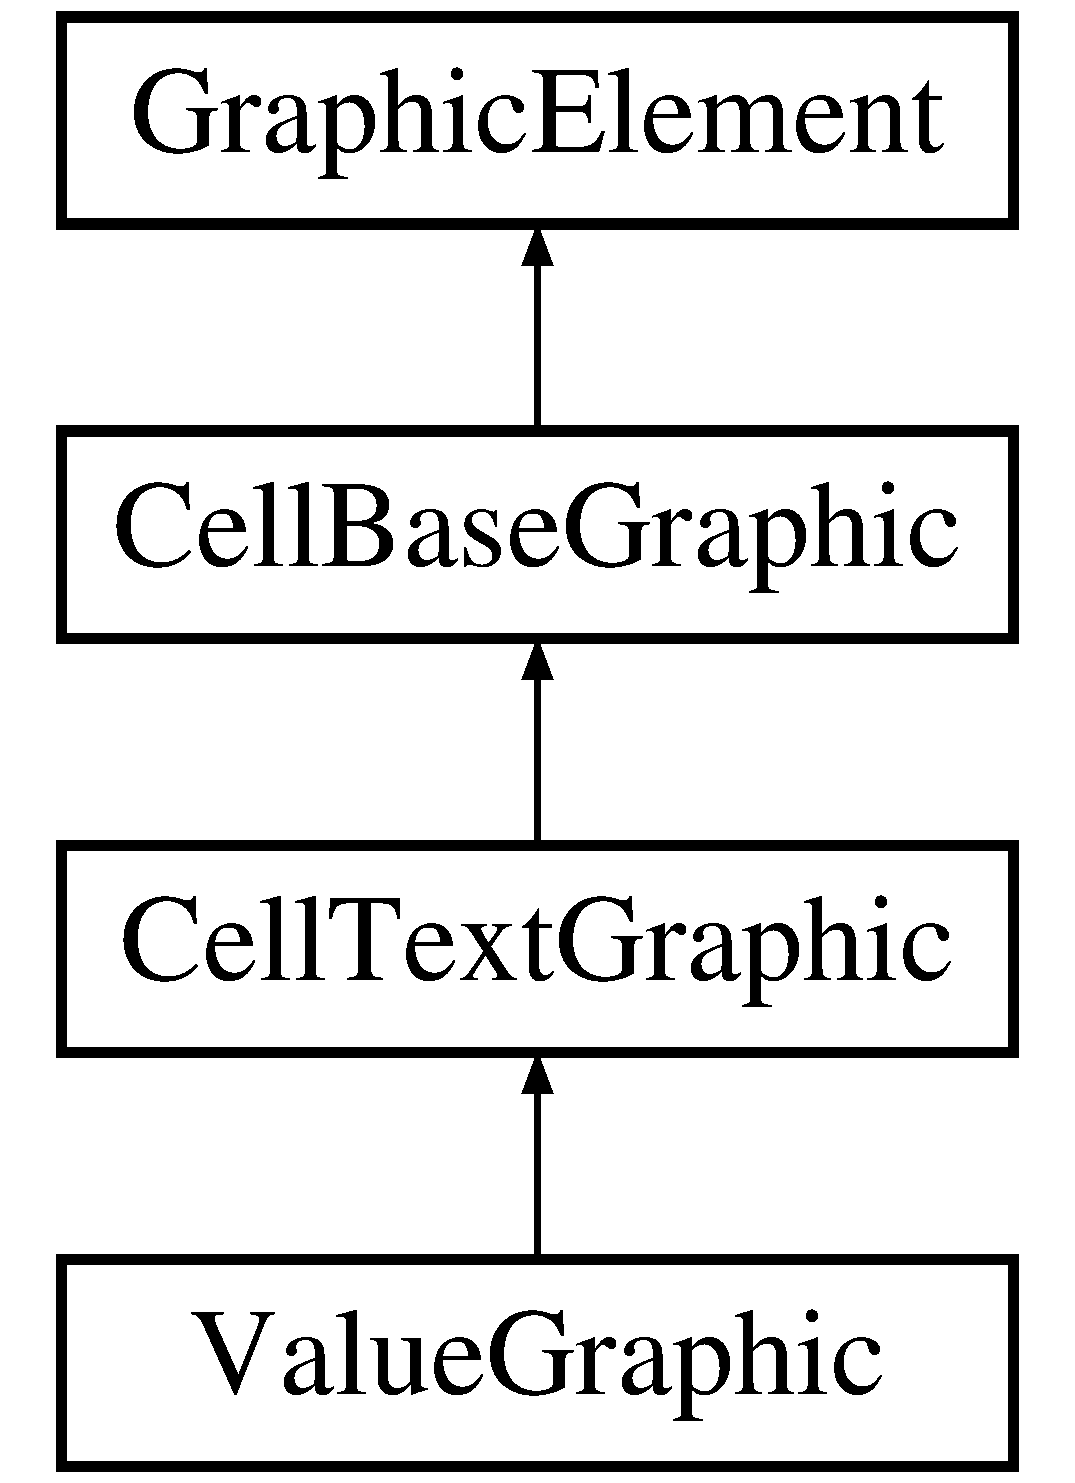
\includegraphics[height=4.000000cm]{class_value_graphic}
\end{center}
\end{figure}
\subsection*{Fonctions membres publiques}
\begin{DoxyCompactItemize}
\item 
\hypertarget{class_value_graphic_ae6fff32502bd90dce5f870fdf644ff1b}{virtual void {\bfseries set\-Image\-To\-Sprite} ()}\label{class_value_graphic_ae6fff32502bd90dce5f870fdf644ff1b}

\end{DoxyCompactItemize}
\subsection*{Membres hérités additionnels}


La documentation de cette classe a été générée à partir des fichiers suivants \-:\begin{DoxyCompactItemize}
\item 
/\-Users/\-Ananas/\-Desktop/\-Mes\-Projets\-Git/purupurudigger/\-Code\-Cpp/Value\-Graphic.\-h\item 
/\-Users/\-Ananas/\-Desktop/\-Mes\-Projets\-Git/purupurudigger/\-Code\-Cpp/Value\-Graphic.\-cpp\end{DoxyCompactItemize}

\chapter{Documentation des fichiers}
\hypertarget{_bomb_8cpp}{\section{Référence du fichier /\-Users/\-Ananas/\-Desktop/\-Mes\-Projets\-Git/purupurudigger/\-Code\-Cpp/\-Bomb.cpp}
\label{_bomb_8cpp}\index{/\-Users/\-Ananas/\-Desktop/\-Mes\-Projets\-Git/purupurudigger/\-Code\-Cpp/\-Bomb.\-cpp@{/\-Users/\-Ananas/\-Desktop/\-Mes\-Projets\-Git/purupurudigger/\-Code\-Cpp/\-Bomb.\-cpp}}
}


Notre classe \hyperlink{class_bomb}{Bomb}.  


{\ttfamily \#include \char`\"{}Bomb.\-h\char`\"{}}\\*


\subsection{Description détaillée}
Notre classe \hyperlink{class_bomb}{Bomb}. \begin{DoxyAuthor}{Auteur}
C\-H\-A\-R\-D\-A\-N Anaël 

D\-A\-M\-E\-Y Jérémy 
\end{DoxyAuthor}
\begin{DoxyDate}{Date}
09/03/2014 
\end{DoxyDate}

\hypertarget{_bomb_8h}{\section{Référence du fichier /\-Users/\-Ananas/\-Desktop/\-Mes\-Projets\-Git/purupurudigger/\-Code\-Cpp/\-Bomb.h}
\label{_bomb_8h}\index{/\-Users/\-Ananas/\-Desktop/\-Mes\-Projets\-Git/purupurudigger/\-Code\-Cpp/\-Bomb.\-h@{/\-Users/\-Ananas/\-Desktop/\-Mes\-Projets\-Git/purupurudigger/\-Code\-Cpp/\-Bomb.\-h}}
}


Notre classe \hyperlink{class_bomb}{Bomb}.  


{\ttfamily \#include $<$iostream$>$}\\*
{\ttfamily \#include \char`\"{}Cell\-Base.\-h\char`\"{}}\\*
\subsection*{Classes}
\begin{DoxyCompactItemize}
\item 
class \hyperlink{class_bomb}{Bomb}
\begin{DoxyCompactList}\small\item\em Classe modélisant ce qu'est une \hyperlink{class_bomb}{Bomb}. \end{DoxyCompactList}\end{DoxyCompactItemize}


\subsection{Description détaillée}
Notre classe \hyperlink{class_bomb}{Bomb}. \begin{DoxyAuthor}{Auteur}
C\-H\-A\-R\-D\-A\-N Anaël 

D\-A\-M\-E\-Y Jérémy 
\end{DoxyAuthor}
\begin{DoxyDate}{Date}
09/03/2014 
\end{DoxyDate}

\hypertarget{_cell_base_8cpp}{\section{Référence du fichier /\-Users/\-Ananas/\-Desktop/\-Mes\-Projets\-Git/purupurudigger/\-Code\-Cpp/\-Cell\-Base.cpp}
\label{_cell_base_8cpp}\index{/\-Users/\-Ananas/\-Desktop/\-Mes\-Projets\-Git/purupurudigger/\-Code\-Cpp/\-Cell\-Base.\-cpp@{/\-Users/\-Ananas/\-Desktop/\-Mes\-Projets\-Git/purupurudigger/\-Code\-Cpp/\-Cell\-Base.\-cpp}}
}


Notre classe \hyperlink{class_cell_base}{Cell\-Base}.  


{\ttfamily \#include \char`\"{}Cell\-Base.\-h\char`\"{}}\\*
{\ttfamily \#include $<$typeinfo$>$}\\*


\subsection{Description détaillée}
Notre classe \hyperlink{class_cell_base}{Cell\-Base}. \begin{DoxyAuthor}{Auteur}
C\-H\-A\-R\-D\-A\-N Anaël 

D\-A\-M\-E\-Y Jérémy 
\end{DoxyAuthor}
\begin{DoxyDate}{Date}
09/03/2014 
\end{DoxyDate}

\hypertarget{_cell_base_8h}{\section{Référence du fichier /\-Users/\-Ananas/\-Desktop/\-Mes\-Projets\-Git/purupurudigger/\-Code\-Cpp/\-Cell\-Base.h}
\label{_cell_base_8h}\index{/\-Users/\-Ananas/\-Desktop/\-Mes\-Projets\-Git/purupurudigger/\-Code\-Cpp/\-Cell\-Base.\-h@{/\-Users/\-Ananas/\-Desktop/\-Mes\-Projets\-Git/purupurudigger/\-Code\-Cpp/\-Cell\-Base.\-h}}
}


Notre classe \hyperlink{class_cell_base}{Cell\-Base}.  


{\ttfamily \#include $<$iostream$>$}\\*
{\ttfamily \#include $<$string$>$}\\*
{\ttfamily \#include \char`\"{}Utils.\-h\char`\"{}}\\*
{\ttfamily \#include \char`\"{}Constantes.\-h\char`\"{}}\\*
\subsection*{Classes}
\begin{DoxyCompactItemize}
\item 
class \hyperlink{class_cell_base}{Cell\-Base}
\begin{DoxyCompactList}\small\item\em Classe modélisant ce qu'est une case. \end{DoxyCompactList}\end{DoxyCompactItemize}


\subsection{Description détaillée}
Notre classe \hyperlink{class_cell_base}{Cell\-Base}. \begin{DoxyAuthor}{Auteur}
C\-H\-A\-R\-D\-A\-N Anaël 

D\-A\-M\-E\-Y Jérémy 
\end{DoxyAuthor}
\begin{DoxyDate}{Date}
09/03/2014 
\end{DoxyDate}

\hypertarget{_constantes_8h}{\section{Référence du fichier /\-Users/\-Ananas/\-Desktop/\-Mes\-Projets\-Git/purupurudigger/\-Code\-Cpp/\-Constantes.h}
\label{_constantes_8h}\index{/\-Users/\-Ananas/\-Desktop/\-Mes\-Projets\-Git/purupurudigger/\-Code\-Cpp/\-Constantes.\-h@{/\-Users/\-Ananas/\-Desktop/\-Mes\-Projets\-Git/purupurudigger/\-Code\-Cpp/\-Constantes.\-h}}
}


Les constantes.  


\subsection*{Énumérations}
\begin{DoxyCompactItemize}
\item 
enum \hyperlink{_constantes_8h_a315ca917ad583797f709ea477dd28705}{Language} \{ \\*
{\bfseries francais}, 
{\bfseries english}, 
{\bfseries deutsch}, 
{\bfseries espanol}, 
\\*
{\bfseries italiano}
 \}
\begin{DoxyCompactList}\small\item\em Voici l'énumeration des différents langues possibles. \end{DoxyCompactList}\item 
enum \hyperlink{_constantes_8h_a4f09127c805cc1f5ee20e67db7b45efa}{Message} \{ \\*
{\bfseries choice}, 
{\bfseries move}, 
{\bfseries nwest}, 
{\bfseries north}, 
\\*
{\bfseries neast}, 
{\bfseries west}, 
{\bfseries east}, 
{\bfseries swest}, 
\\*
{\bfseries south}, 
{\bfseries seast}, 
{\bfseries stop}, 
{\bfseries score}, 
\\*
{\bfseries level}, 
{\bfseries global}, 
{\bfseries current}, 
{\bfseries goal}, 
\\*
{\bfseries step}, 
{\bfseries life}, 
{\bfseries position}, 
{\bfseries winlevel}, 
\\*
{\bfseries looselevel}, 
{\bfseries loosegame}, 
{\bfseries name}, 
{\bfseries ltime}, 
\\*
{\bfseries timeup}, 
{\bfseries by}, 
{\bfseries play}, 
{\bfseries best}, 
\\*
{\bfseries setting}, 
{\bfseries language}, 
{\bfseries actual}, 
{\bfseries theme}
 \}
\begin{DoxyCompactList}\small\item\em Voici l'énumeration des différents messages possibles. \end{DoxyCompactList}\item 
enum {\bfseries Movement} \{ \\*
{\bfseries Nwest}, 
{\bfseries N\-East}, 
{\bfseries North}, 
{\bfseries South}, 
\\*
{\bfseries S\-West}, 
{\bfseries S\-East}, 
{\bfseries West}, 
{\bfseries East}
 \}
\end{DoxyCompactItemize}
\subsection*{Variables}
\begin{DoxyCompactItemize}
\item 
\hypertarget{_constantes_8h_ae45bf4c0e6b1d99fc99e157f74cb1ea0}{const int {\bfseries C\-O\-L\-O\-N\-N\-E} = 18}\label{_constantes_8h_ae45bf4c0e6b1d99fc99e157f74cb1ea0}

\item 
\hypertarget{_constantes_8h_a9f34eefe6819ddccaeb86da8bb65360a}{const int {\bfseries L\-I\-G\-N\-E} = 18}\label{_constantes_8h_a9f34eefe6819ddccaeb86da8bb65360a}

\item 
\hypertarget{_constantes_8h_a71fe1a78debc30125710b2a01b1663a8}{const int {\bfseries M\-I\-N\-V\-A\-L} = 1}\label{_constantes_8h_a71fe1a78debc30125710b2a01b1663a8}

\item 
\hypertarget{_constantes_8h_afbd3bad1d9da6b7935af1714d415c6c1}{const int {\bfseries M\-A\-X\-V\-A\-L} = 6}\label{_constantes_8h_afbd3bad1d9da6b7935af1714d415c6c1}

\item 
\hypertarget{_constantes_8h_a605058debdf7d118d06045856908d667}{const int {\bfseries M\-I\-N\-O\-B\-J} = 8}\label{_constantes_8h_a605058debdf7d118d06045856908d667}

\item 
\hypertarget{_constantes_8h_aa0662d0b34143a209aa4dfacd926cb38}{const int {\bfseries M\-A\-X\-O\-B\-J} = 10}\label{_constantes_8h_aa0662d0b34143a209aa4dfacd926cb38}

\item 
\hypertarget{_constantes_8h_a46ddfdc4e3be45b06f82bf9beabe43aa}{const int {\bfseries M\-I\-N\-V\-A\-L\-B} = 10}\label{_constantes_8h_a46ddfdc4e3be45b06f82bf9beabe43aa}

\item 
\hypertarget{_constantes_8h_a2fa7e505c01a24ad72efda083ca7170f}{const int {\bfseries M\-A\-X\-V\-A\-L\-B} = 100}\label{_constantes_8h_a2fa7e505c01a24ad72efda083ca7170f}

\item 
\hypertarget{_constantes_8h_a1849725ee55eae115e3000bf552dee51}{const int {\bfseries R\-E\-D} = 31}\label{_constantes_8h_a1849725ee55eae115e3000bf552dee51}

\item 
\hypertarget{_constantes_8h_a05bf83136788998dddf9143bcc8d4cbd}{const int {\bfseries G\-R\-E\-E\-N} = 32}\label{_constantes_8h_a05bf83136788998dddf9143bcc8d4cbd}

\item 
\hypertarget{_constantes_8h_ae55fbbfbc6852abe60a45bea8922b225}{const int {\bfseries Y\-E\-L\-L\-O\-W} = 33}\label{_constantes_8h_ae55fbbfbc6852abe60a45bea8922b225}

\item 
\hypertarget{_constantes_8h_aa98874749cfc133195b5ceffd6f583e7}{const int {\bfseries B\-L\-U\-E} = 34}\label{_constantes_8h_aa98874749cfc133195b5ceffd6f583e7}

\item 
\hypertarget{_constantes_8h_aba659bcba3358aadd16f9b90982a4cf1}{const int {\bfseries P\-I\-N\-K} = 35}\label{_constantes_8h_aba659bcba3358aadd16f9b90982a4cf1}

\item 
\hypertarget{_constantes_8h_a2db88b0cae6c6b4e4f291837a1213c5e}{const int {\bfseries C\-Y\-A\-N} = 36}\label{_constantes_8h_a2db88b0cae6c6b4e4f291837a1213c5e}

\item 
\hypertarget{_constantes_8h_a6fdc54ca55874b2959f7d77967f78dc2}{const int {\bfseries W\-H\-I\-T\-E} = 37}\label{_constantes_8h_a6fdc54ca55874b2959f7d77967f78dc2}

\item 
\hypertarget{_constantes_8h_a1b917f3b9c66922034e640c9a04c256c}{const int {\bfseries W\-I\-N\-D\-O\-W\-W\-I\-T\-D\-H} = 1128}\label{_constantes_8h_a1b917f3b9c66922034e640c9a04c256c}

\item 
\hypertarget{_constantes_8h_a69a6fba51c529e022587f8e9f27eaa2d}{const int {\bfseries W\-I\-N\-D\-O\-W\-H\-E\-I\-G\-H\-T} = 828}\label{_constantes_8h_a69a6fba51c529e022587f8e9f27eaa2d}

\item 
\hypertarget{_constantes_8h_a748df152d56e5d3e313573e5cbd4080f}{const int {\bfseries B\-P\-P} = 32}\label{_constantes_8h_a748df152d56e5d3e313573e5cbd4080f}

\item 
\hypertarget{_constantes_8h_a98f244d2ed45908f208c3f70b801304b}{const int {\bfseries M\-A\-R\-G\-I\-N\-L\-E\-F\-T} = 400}\label{_constantes_8h_a98f244d2ed45908f208c3f70b801304b}

\item 
\hypertarget{_constantes_8h_a59a2a34d231a812dd6e59b65500bfc2f}{const int {\bfseries M\-A\-R\-G\-I\-N\-T\-O\-P} = 100}\label{_constantes_8h_a59a2a34d231a812dd6e59b65500bfc2f}

\item 
\hypertarget{_constantes_8h_a7c58a3afb6f12e71dd4e17e88f787fa9}{const int {\bfseries P\-A\-D\-D\-I\-N\-G\-R\-I\-G\-H\-T} = 3}\label{_constantes_8h_a7c58a3afb6f12e71dd4e17e88f787fa9}

\item 
\hypertarget{_constantes_8h_a300a304652bed5ac81dd9eee4d795b11}{const int {\bfseries P\-A\-D\-D\-I\-N\-G\-B\-O\-T\-T\-O\-M} = 3}\label{_constantes_8h_a300a304652bed5ac81dd9eee4d795b11}

\item 
\hypertarget{_constantes_8h_a48c8e2d01ca921cf58cad85b2e4dbbc1}{const int {\bfseries C\-A\-S\-E\-W\-I\-T\-D\-H} = 35}\label{_constantes_8h_a48c8e2d01ca921cf58cad85b2e4dbbc1}

\item 
\hypertarget{_constantes_8h_a7c9068f654a9984eef4346cdb511dec1}{const int {\bfseries C\-A\-S\-E\-H\-E\-I\-G\-H\-T} = 35}\label{_constantes_8h_a7c9068f654a9984eef4346cdb511dec1}

\item 
\hypertarget{_constantes_8h_adc26e878f2ab67b8bacb78b82d5cdfc6}{const int {\bfseries S\-P\-R\-I\-T\-E\-C\-A\-S\-E\-B\-E\-G\-I\-N} = 6}\label{_constantes_8h_adc26e878f2ab67b8bacb78b82d5cdfc6}

\item 
\hypertarget{_constantes_8h_a0e763e322fcb44f2c7b8177ad9741974}{const int {\bfseries S\-P\-R\-I\-T\-E\-C\-A\-S\-E\-H\-E\-I\-G\-H\-T} = 56}\label{_constantes_8h_a0e763e322fcb44f2c7b8177ad9741974}

\item 
\hypertarget{_constantes_8h_aafedcfa2a91e170257cf3be9914ccf93}{const int {\bfseries D\-I\-G\-G\-E\-R\-S\-X} = 0}\label{_constantes_8h_aafedcfa2a91e170257cf3be9914ccf93}

\item 
\hypertarget{_constantes_8h_a37589c3784f6e3f5990dc4ca5722e4f6}{const int {\bfseries D\-I\-G\-G\-E\-R\-E\-X} = 50}\label{_constantes_8h_a37589c3784f6e3f5990dc4ca5722e4f6}

\item 
\hypertarget{_constantes_8h_a192ede5a1fe4f22f5765f3ad0c658207}{const int {\bfseries G\-O\-L\-D\-S\-X} = 56}\label{_constantes_8h_a192ede5a1fe4f22f5765f3ad0c658207}

\item 
\hypertarget{_constantes_8h_a2d02af819c2bdd8ee384fbec8ca83b87}{const int {\bfseries G\-O\-L\-D\-E\-X} = 106}\label{_constantes_8h_a2d02af819c2bdd8ee384fbec8ca83b87}

\item 
\hypertarget{_constantes_8h_a7cdb38aa6f23d233c3a2b988ff27e5dd}{const int {\bfseries E\-M\-P\-T\-Y\-S\-X} = 112}\label{_constantes_8h_a7cdb38aa6f23d233c3a2b988ff27e5dd}

\item 
\hypertarget{_constantes_8h_abd7b74616f723b171d11cbc6f126f431}{const int {\bfseries E\-M\-P\-T\-Y\-E\-X} = 162}\label{_constantes_8h_abd7b74616f723b171d11cbc6f126f431}

\item 
\hypertarget{_constantes_8h_aa58e425eb3e620563e0052433e641c52}{const int {\bfseries B\-O\-M\-B\-S\-X} = 168}\label{_constantes_8h_aa58e425eb3e620563e0052433e641c52}

\item 
\hypertarget{_constantes_8h_afb6b9a495ec236907901995c4af3b5cb}{const int {\bfseries B\-O\-M\-B\-E\-X} = 218}\label{_constantes_8h_afb6b9a495ec236907901995c4af3b5cb}

\item 
\hypertarget{_constantes_8h_ad5fd743d4e52be0e5205d8974ee32839}{const int {\bfseries V\-A\-L\-U\-E\-S\-X} = 224}\label{_constantes_8h_ad5fd743d4e52be0e5205d8974ee32839}

\item 
\hypertarget{_constantes_8h_ab39f4d3c453a4e25fc3a17ab4abf0da3}{const int {\bfseries V\-A\-L\-U\-E\-E\-X} = 274}\label{_constantes_8h_ab39f4d3c453a4e25fc3a17ab4abf0da3}

\item 
\hypertarget{_constantes_8h_a395a09a9ead33dbc8ff069013f861dd9}{const int {\bfseries T\-E\-X\-T\-P\-L\-A\-C\-E\-X} = 150}\label{_constantes_8h_a395a09a9ead33dbc8ff069013f861dd9}

\item 
\hypertarget{_constantes_8h_acc8327a09d4c2f48d1ebb3e19b04bab7}{const int {\bfseries S\-P\-R\-I\-T\-E\-L\-A\-N\-G\-U\-E\-B\-E\-G\-I\-N} = 12}\label{_constantes_8h_acc8327a09d4c2f48d1ebb3e19b04bab7}

\item 
\hypertarget{_constantes_8h_afbaf7c1dbaebc06c67c6da0562690b94}{const int {\bfseries S\-P\-R\-I\-T\-E\-L\-A\-N\-G\-U\-E\-H\-E\-I\-G\-H\-T} = 122}\label{_constantes_8h_afbaf7c1dbaebc06c67c6da0562690b94}

\item 
\hypertarget{_constantes_8h_a62591aa497170e2428b6e736568ab69e}{const int {\bfseries L\-A\-N\-G\-U\-E\-W\-I\-D\-T\-H} = 50}\label{_constantes_8h_a62591aa497170e2428b6e736568ab69e}

\item 
\hypertarget{_constantes_8h_a97eec71f67c97c1d2bdc34cf7ebf279e}{const int {\bfseries L\-A\-N\-G\-U\-E\-H\-E\-I\-G\-H\-T} = 50}\label{_constantes_8h_a97eec71f67c97c1d2bdc34cf7ebf279e}

\item 
\hypertarget{_constantes_8h_a2f5055fc3128d61ade2230e72b912ae1}{const int {\bfseries C\-H\-O\-I\-C\-E\-L\-A\-N\-G\-U\-E\-H\-I\-G\-H} = 150}\label{_constantes_8h_a2f5055fc3128d61ade2230e72b912ae1}

\item 
\hypertarget{_constantes_8h_a8da8cf2cf6f12f1d1e04c195c56c0752}{const int {\bfseries M\-Y\-L\-A\-N\-G\-U\-E\-X} = 400}\label{_constantes_8h_a8da8cf2cf6f12f1d1e04c195c56c0752}

\item 
\hypertarget{_constantes_8h_a1618b37b8fb6b4373b7853c951ceebb1}{const int {\bfseries M\-Y\-L\-A\-N\-G\-U\-E\-Y} = C\-H\-O\-I\-C\-E\-L\-A\-N\-G\-U\-E\-H\-I\-G\-H + 120}\label{_constantes_8h_a1618b37b8fb6b4373b7853c951ceebb1}

\item 
\hypertarget{_constantes_8h_a27b49db0b8cf04eb87fb8bf6751c9dba}{const int {\bfseries E\-N\-G\-L\-I\-S\-H\-X} = 400}\label{_constantes_8h_a27b49db0b8cf04eb87fb8bf6751c9dba}

\item 
\hypertarget{_constantes_8h_af85490e77fa2177ecc0c91dc2166028a}{const int {\bfseries E\-N\-G\-L\-I\-S\-H\-S\-X} = 7}\label{_constantes_8h_af85490e77fa2177ecc0c91dc2166028a}

\item 
\hypertarget{_constantes_8h_a5d87cdcb293f2f860cd748acc004a17b}{const int {\bfseries E\-N\-G\-L\-I\-S\-H\-E\-X} = 114}\label{_constantes_8h_a5d87cdcb293f2f860cd748acc004a17b}

\item 
\hypertarget{_constantes_8h_a9441c4b468e6385486ac450fe80e6f78}{const int {\bfseries F\-R\-E\-N\-C\-H\-X} = E\-N\-G\-L\-I\-S\-H\-X + 100}\label{_constantes_8h_a9441c4b468e6385486ac450fe80e6f78}

\item 
\hypertarget{_constantes_8h_a6ba3fef4a21ed6743a87f5aad639520e}{const int {\bfseries F\-R\-E\-N\-C\-H\-S\-X} = 123}\label{_constantes_8h_a6ba3fef4a21ed6743a87f5aad639520e}

\item 
\hypertarget{_constantes_8h_a5f1c3ac92c19a20e68e6ca5c03f4fcd7}{const int {\bfseries F\-R\-E\-N\-C\-H\-E\-X} = 230}\label{_constantes_8h_a5f1c3ac92c19a20e68e6ca5c03f4fcd7}

\item 
\hypertarget{_constantes_8h_a0ddb80810a7344217091610c0b219e4b}{const int {\bfseries I\-T\-A\-L\-I\-A\-N\-O\-X} = F\-R\-E\-N\-C\-H\-X + 100}\label{_constantes_8h_a0ddb80810a7344217091610c0b219e4b}

\item 
\hypertarget{_constantes_8h_a869f10e4030bcd666c1efa4d6a47394f}{const int {\bfseries I\-T\-A\-L\-I\-A\-N\-O\-S\-X} = 240}\label{_constantes_8h_a869f10e4030bcd666c1efa4d6a47394f}

\item 
\hypertarget{_constantes_8h_a2659ef86f752dc8f4bf1271400d2801a}{const int {\bfseries I\-T\-A\-L\-I\-A\-N\-O\-E\-X} = 346}\label{_constantes_8h_a2659ef86f752dc8f4bf1271400d2801a}

\item 
\hypertarget{_constantes_8h_af023436c54d4acfe209edabba6d72676}{const int {\bfseries S\-P\-A\-N\-I\-S\-H\-X} = I\-T\-A\-L\-I\-A\-N\-O\-X + 100}\label{_constantes_8h_af023436c54d4acfe209edabba6d72676}

\item 
\hypertarget{_constantes_8h_a88663c40d8db6db3bfef67a8ce3c56ca}{const int {\bfseries S\-P\-A\-N\-I\-S\-H\-S\-X} = 360}\label{_constantes_8h_a88663c40d8db6db3bfef67a8ce3c56ca}

\item 
\hypertarget{_constantes_8h_a0f5ae72fe0f52c8549073d35f308943d}{const int {\bfseries S\-P\-A\-N\-I\-S\-H\-E\-X} = 463}\label{_constantes_8h_a0f5ae72fe0f52c8549073d35f308943d}

\item 
\hypertarget{_constantes_8h_a3daca1c6a5d3ae81e8f63df850705945}{const int {\bfseries D\-E\-U\-T\-S\-C\-H\-X} = S\-P\-A\-N\-I\-S\-H\-X + 100}\label{_constantes_8h_a3daca1c6a5d3ae81e8f63df850705945}

\item 
\hypertarget{_constantes_8h_ab8f3c8abc5d2839e9a9a77d173b09c62}{const int {\bfseries D\-E\-U\-T\-S\-C\-H\-S\-X} = 472}\label{_constantes_8h_ab8f3c8abc5d2839e9a9a77d173b09c62}

\item 
\hypertarget{_constantes_8h_a7ca60ed2196dfc29ed3a96ef21afacfa}{const int {\bfseries D\-E\-U\-T\-S\-C\-H\-E\-X} = 578}\label{_constantes_8h_a7ca60ed2196dfc29ed3a96ef21afacfa}

\item 
\hypertarget{_constantes_8h_abbff6b115a9d6ed89a20060f48a4b7dd}{const int {\bfseries C\-H\-O\-I\-C\-E\-S\-P\-R\-I\-T\-E\-Y} = M\-Y\-L\-A\-N\-G\-U\-E\-Y + 120}\label{_constantes_8h_abbff6b115a9d6ed89a20060f48a4b7dd}

\item 
\hypertarget{_constantes_8h_a42c366303eb11249f43efe2ae0b0483c}{const int {\bfseries C\-H\-O\-I\-C\-E\-A\-N\-A\-N\-A\-S\-X} = 400}\label{_constantes_8h_a42c366303eb11249f43efe2ae0b0483c}

\item 
\hypertarget{_constantes_8h_a3545dfe9df6133b1e1d9f6d8d15d1a4f}{const int {\bfseries C\-H\-O\-I\-C\-E\-T\-E\-A\-C\-H\-E\-R\-X} = 700}\label{_constantes_8h_a3545dfe9df6133b1e1d9f6d8d15d1a4f}

\item 
\hypertarget{_constantes_8h_ac3a4f53b42dcf7c63612c7c9baa4dba0}{const int {\bfseries S\-P\-R\-I\-T\-E\-C\-H\-O\-I\-C\-E\-B\-E\-G\-I\-N} = 0}\label{_constantes_8h_ac3a4f53b42dcf7c63612c7c9baa4dba0}

\item 
\hypertarget{_constantes_8h_a1222f65f86c505eb2071fc74b09a6e6f}{const int {\bfseries S\-P\-R\-I\-T\-E\-C\-H\-O\-I\-C\-E\-H\-E\-I\-G\-H\-T} = 150}\label{_constantes_8h_a1222f65f86c505eb2071fc74b09a6e6f}

\item 
\hypertarget{_constantes_8h_aa60bbd1b6bc7705c91b5b4d72af9f217}{const int {\bfseries S\-P\-R\-I\-T\-E\-C\-H\-O\-I\-C\-E\-W\-I\-D\-T\-H} = 150}\label{_constantes_8h_aa60bbd1b6bc7705c91b5b4d72af9f217}

\item 
\hypertarget{_constantes_8h_af81d1dbbd9dcb0fb35a80bc8b7a5acce}{const int {\bfseries S\-P\-R\-I\-T\-E\-A\-N\-A\-N\-A\-S\-S\-X} = 0}\label{_constantes_8h_af81d1dbbd9dcb0fb35a80bc8b7a5acce}

\item 
\hypertarget{_constantes_8h_ac3652f5ace5f6855be4e5173ab2a6217}{const int {\bfseries S\-P\-R\-I\-T\-E\-A\-N\-A\-N\-A\-S\-E\-X} = 285}\label{_constantes_8h_ac3652f5ace5f6855be4e5173ab2a6217}

\item 
\hypertarget{_constantes_8h_aaf8cc554e46d59216fba54a32e3815ad}{const int {\bfseries S\-P\-R\-I\-T\-E\-T\-E\-A\-C\-H\-E\-R\-S\-X} = 344}\label{_constantes_8h_aaf8cc554e46d59216fba54a32e3815ad}

\item 
\hypertarget{_constantes_8h_ad51b431cf1b40d0efcc7f133ae85f14b}{const int {\bfseries S\-P\-R\-I\-T\-E\-T\-E\-A\-C\-H\-E\-R\-E\-X} = 600}\label{_constantes_8h_ad51b431cf1b40d0efcc7f133ae85f14b}

\item 
\hypertarget{_constantes_8h_a3e01f17dfdf93d4916fc63a6a1abd79c}{const int {\bfseries B\-U\-T\-T\-O\-N\-W\-I\-D\-T\-H} = 220}\label{_constantes_8h_a3e01f17dfdf93d4916fc63a6a1abd79c}

\item 
\hypertarget{_constantes_8h_a2fcf486492665ea07bfd475dc0f85a3f}{const int {\bfseries B\-U\-T\-T\-O\-N\-H\-E\-I\-G\-H\-T} = 60}\label{_constantes_8h_a2fcf486492665ea07bfd475dc0f85a3f}

\item 
\hypertarget{_constantes_8h_a40ea952dab8229c4d40070bdd93a7b4d}{const int {\bfseries B\-U\-T\-T\-O\-N\-C\-A\-S\-E\-B\-E\-G\-I\-N} = 3}\label{_constantes_8h_a40ea952dab8229c4d40070bdd93a7b4d}

\item 
\hypertarget{_constantes_8h_a0ca7ee75bd29a31e65c4d76ddad2bd0c}{const int {\bfseries B\-U\-T\-T\-O\-N\-C\-A\-S\-E\-H\-E\-I\-G\-H\-T} = 68}\label{_constantes_8h_a0ca7ee75bd29a31e65c4d76ddad2bd0c}

\item 
\hypertarget{_constantes_8h_a2333d1922183ecab66ed917ca83c7962}{const int {\bfseries B\-U\-T\-T\-O\-N\-N\-O\-R\-M\-S\-X} = 2}\label{_constantes_8h_a2333d1922183ecab66ed917ca83c7962}

\item 
\hypertarget{_constantes_8h_a688f6cc68e37520686fd95425a108f1e}{const int {\bfseries B\-U\-T\-T\-O\-N\-N\-O\-R\-M\-E\-X} = 143}\label{_constantes_8h_a688f6cc68e37520686fd95425a108f1e}

\item 
\hypertarget{_constantes_8h_a7e553ef4dd51ffdbd3f8e49ff7a29d6f}{const int {\bfseries B\-U\-T\-T\-O\-N\-H\-O\-V\-E\-S\-X} = 157}\label{_constantes_8h_a7e553ef4dd51ffdbd3f8e49ff7a29d6f}

\item 
\hypertarget{_constantes_8h_a0ac639a40f107230737e3214d75ccde3}{const int {\bfseries B\-U\-T\-T\-O\-N\-H\-O\-V\-E\-E\-X} = 298}\label{_constantes_8h_a0ac639a40f107230737e3214d75ccde3}

\item 
\hypertarget{_constantes_8h_adcc36a93647e553517df78d4fcccb591}{const int {\bfseries I\-C\-O\-N\-W\-I\-D\-T\-H} = 50}\label{_constantes_8h_adcc36a93647e553517df78d4fcccb591}

\item 
\hypertarget{_constantes_8h_ab7a8b45ccfaa0328a40790fb77e21a51}{const int {\bfseries I\-C\-O\-N\-H\-E\-I\-G\-H\-T} = 50}\label{_constantes_8h_ab7a8b45ccfaa0328a40790fb77e21a51}

\item 
\hypertarget{_constantes_8h_a9972bc27df55821f9d9034ca926fa74e}{const int {\bfseries I\-C\-O\-N\-S\-P\-R\-I\-T\-E\-B\-E\-G\-I\-N} = 0}\label{_constantes_8h_a9972bc27df55821f9d9034ca926fa74e}

\item 
\hypertarget{_constantes_8h_a32e01d105b7ead087b20d5415ef1f731}{const int {\bfseries I\-C\-O\-N\-S\-P\-R\-I\-T\-E\-H\-E\-I\-G\-H\-T} = 143}\label{_constantes_8h_a32e01d105b7ead087b20d5415ef1f731}

\item 
\hypertarget{_constantes_8h_afa52cb626e7fac1da537f4ec8f6611a5}{const int {\bfseries M\-U\-S\-I\-C\-O\-N\-S\-X} = 0}\label{_constantes_8h_afa52cb626e7fac1da537f4ec8f6611a5}

\item 
\hypertarget{_constantes_8h_a9590eab159e25d89e1f0f3d173fa2d82}{const int {\bfseries M\-U\-S\-I\-C\-O\-N\-E\-X} = 130}\label{_constantes_8h_a9590eab159e25d89e1f0f3d173fa2d82}

\item 
\hypertarget{_constantes_8h_a6edd99cdc12c099459875fbb24f9a16b}{const int {\bfseries M\-U\-S\-I\-C\-O\-F\-F\-S\-X} = 130}\label{_constantes_8h_a6edd99cdc12c099459875fbb24f9a16b}

\item 
\hypertarget{_constantes_8h_a69998dea9e002866e4a3cd9c70ae93d3}{const int {\bfseries M\-U\-S\-I\-C\-O\-F\-F\-E\-X} = 270}\label{_constantes_8h_a69998dea9e002866e4a3cd9c70ae93d3}

\item 
\hypertarget{_constantes_8h_a1784053244c6a14dbb7fd1288a561373}{const int {\bfseries S\-O\-U\-N\-D\-S\-X} = 270}\label{_constantes_8h_a1784053244c6a14dbb7fd1288a561373}

\item 
\hypertarget{_constantes_8h_a2b0b1ca2754fa4e8a4ff3f62b96d6444}{const int {\bfseries S\-O\-U\-N\-D\-O\-F\-F\-E\-X} = 370}\label{_constantes_8h_a2b0b1ca2754fa4e8a4ff3f62b96d6444}

\item 
\hypertarget{_constantes_8h_acce866145e142c7c0637c4284240f4ab}{const int {\bfseries S\-O\-U\-N\-D\-O\-N\-E\-X} = 431}\label{_constantes_8h_acce866145e142c7c0637c4284240f4ab}

\item 
\hypertarget{_constantes_8h_a6c2879b33cb7aef05ca43ec89e678423}{const int {\bfseries I\-C\-O\-N\-Y} = 10}\label{_constantes_8h_a6c2879b33cb7aef05ca43ec89e678423}

\item 
\hypertarget{_constantes_8h_a8c54d319b6e5afa9868f6ae27d4bc583}{const int {\bfseries M\-U\-S\-I\-C\-X} = W\-I\-N\-D\-O\-W\-W\-I\-T\-D\-H -\/ ( 2 $\ast$ I\-C\-O\-N\-W\-I\-D\-T\-H ) -\/ 100}\label{_constantes_8h_a8c54d319b6e5afa9868f6ae27d4bc583}

\item 
\hypertarget{_constantes_8h_a4c97f22e5a5c5cca4d1804609e6c513e}{const int {\bfseries S\-O\-U\-N\-D\-X} = M\-U\-S\-I\-C\-X + I\-C\-O\-N\-W\-I\-D\-T\-H + 20}\label{_constantes_8h_a4c97f22e5a5c5cca4d1804609e6c513e}

\item 
\hypertarget{_constantes_8h_a745543f54d99966644d162e2f9d0f171}{const int {\bfseries P\-L\-A\-Y\-X} = 150}\label{_constantes_8h_a745543f54d99966644d162e2f9d0f171}

\item 
\hypertarget{_constantes_8h_a3eadd5690f40c938f7ed257d7d885fde}{const int {\bfseries P\-L\-A\-Y\-Y} = 300}\label{_constantes_8h_a3eadd5690f40c938f7ed257d7d885fde}

\item 
\hypertarget{_constantes_8h_a51afff60951dbe3088d18a1c4279c641}{const int {\bfseries O\-P\-T\-I\-O\-N\-X} = P\-L\-A\-Y\-X + 200}\label{_constantes_8h_a51afff60951dbe3088d18a1c4279c641}

\item 
\hypertarget{_constantes_8h_a5df88094b301f0c26248f52fbf2c734a}{const int {\bfseries O\-P\-T\-I\-O\-N\-Y} = P\-L\-A\-Y\-Y + 120}\label{_constantes_8h_a5df88094b301f0c26248f52fbf2c734a}

\item 
\hypertarget{_constantes_8h_a94a08ae35c368aa88ccec10a455b050f}{const int {\bfseries B\-E\-S\-T\-X} = O\-P\-T\-I\-O\-N\-X + 200}\label{_constantes_8h_a94a08ae35c368aa88ccec10a455b050f}

\item 
\hypertarget{_constantes_8h_a942b0731f92c91ac7ab9827ff9b777be}{const int {\bfseries B\-E\-S\-T\-Y} = O\-P\-T\-I\-O\-N\-Y + 120}\label{_constantes_8h_a942b0731f92c91ac7ab9827ff9b777be}

\item 
\hypertarget{_constantes_8h_a1d2baa2233bd8d19812af09dc29b8c46}{const int {\bfseries Q\-U\-I\-T\-X} = B\-E\-S\-T\-X + 200}\label{_constantes_8h_a1d2baa2233bd8d19812af09dc29b8c46}

\item 
\hypertarget{_constantes_8h_aa76d69bd0b57032480aa421c390a4cc3}{const int {\bfseries Q\-U\-I\-T\-Y} = B\-E\-S\-T\-Y + 120}\label{_constantes_8h_aa76d69bd0b57032480aa421c390a4cc3}

\item 
\hypertarget{_constantes_8h_a9db7806522bc79c49c2ba616da82c928}{const int {\bfseries Q\-U\-I\-T\-O\-N\-X} = 100}\label{_constantes_8h_a9db7806522bc79c49c2ba616da82c928}

\item 
\hypertarget{_constantes_8h_acaf704dd6f70d41cf6285dd45a731ad6}{const int {\bfseries Q\-U\-I\-T\-O\-N\-Y} = 600}\label{_constantes_8h_acaf704dd6f70d41cf6285dd45a731ad6}

\item 
\hypertarget{_constantes_8h_a76497367551ca56ead4b9910a5536c2a}{const std\-::string {\bfseries F\-I\-L\-E\-B\-E\-S\-T\-S\-C\-O\-R\-E} = \char`\"{}best\-Scores.\-txt\char`\"{}}\label{_constantes_8h_a76497367551ca56ead4b9910a5536c2a}

\end{DoxyCompactItemize}


\subsection{Description détaillée}
Les constantes. \begin{DoxyAuthor}{Auteur}
C\-H\-A\-R\-D\-A\-N Anaël 

D\-A\-M\-E\-Y Jérémy 
\end{DoxyAuthor}
\begin{DoxyDate}{Date}
09/03/2014 
\end{DoxyDate}

\hypertarget{_digger_8cpp}{\section{Référence du fichier /\-Users/\-Ananas/\-Desktop/\-Mes\-Projets\-Git/purupurudigger/\-Code\-Cpp/\-Digger.cpp}
\label{_digger_8cpp}\index{/\-Users/\-Ananas/\-Desktop/\-Mes\-Projets\-Git/purupurudigger/\-Code\-Cpp/\-Digger.\-cpp@{/\-Users/\-Ananas/\-Desktop/\-Mes\-Projets\-Git/purupurudigger/\-Code\-Cpp/\-Digger.\-cpp}}
}


Notre classe \hyperlink{class_digger}{Digger}.  


{\ttfamily \#include \char`\"{}Digger.\-h\char`\"{}}\\*
{\ttfamily \#include \char`\"{}Constantes.\-h\char`\"{}}\\*


\subsection{Description détaillée}
Notre classe \hyperlink{class_digger}{Digger}. \begin{DoxyAuthor}{Auteur}
C\-H\-A\-R\-D\-A\-N Anaël 

D\-A\-M\-E\-Y Jérémy 
\end{DoxyAuthor}
\begin{DoxyDate}{Date}
09/03/2014 
\end{DoxyDate}

\hypertarget{_digger_8h}{\section{Référence du fichier /\-Users/\-Ananas/\-Desktop/\-Mes\-Projets\-Git/purupurudigger/\-Code\-Cpp/\-Digger.h}
\label{_digger_8h}\index{/\-Users/\-Ananas/\-Desktop/\-Mes\-Projets\-Git/purupurudigger/\-Code\-Cpp/\-Digger.\-h@{/\-Users/\-Ananas/\-Desktop/\-Mes\-Projets\-Git/purupurudigger/\-Code\-Cpp/\-Digger.\-h}}
}


Notre classe \hyperlink{class_digger}{Digger}.  


{\ttfamily \#include $<$iostream$>$}\\*
{\ttfamily \#include \char`\"{}Cell\-Base.\-h\char`\"{}}\\*
\subsection*{Classes}
\begin{DoxyCompactItemize}
\item 
class \hyperlink{class_digger}{Digger}
\begin{DoxyCompactList}\small\item\em Classe modélisant ce qu'est un digger. \end{DoxyCompactList}\end{DoxyCompactItemize}


\subsection{Description détaillée}
Notre classe \hyperlink{class_digger}{Digger}. \begin{DoxyAuthor}{Auteur}
C\-H\-A\-R\-D\-A\-N Anaël 

D\-A\-M\-E\-Y Jérémy 
\end{DoxyAuthor}
\begin{DoxyDate}{Date}
09/03/2014 
\end{DoxyDate}

\hypertarget{_empty_cell_8cpp}{\section{Référence du fichier /\-Users/\-Ananas/\-Desktop/\-Mes\-Projets\-Git/purupurudigger/\-Code\-Cpp/\-Empty\-Cell.cpp}
\label{_empty_cell_8cpp}\index{/\-Users/\-Ananas/\-Desktop/\-Mes\-Projets\-Git/purupurudigger/\-Code\-Cpp/\-Empty\-Cell.\-cpp@{/\-Users/\-Ananas/\-Desktop/\-Mes\-Projets\-Git/purupurudigger/\-Code\-Cpp/\-Empty\-Cell.\-cpp}}
}


Notre classe \hyperlink{class_empty_cell}{Empty\-Cell}.  


{\ttfamily \#include \char`\"{}Empty\-Cell.\-h\char`\"{}}\\*


\subsection{Description détaillée}
Notre classe \hyperlink{class_empty_cell}{Empty\-Cell}. \begin{DoxyAuthor}{Auteur}
C\-H\-A\-R\-D\-A\-N Anaël 

D\-A\-M\-E\-Y Jérémy 
\end{DoxyAuthor}
\begin{DoxyDate}{Date}
09/03/2014 
\end{DoxyDate}

\hypertarget{_empty_cell_8h}{\section{Référence du fichier /\-Users/\-Ananas/\-Desktop/\-Mes\-Projets\-Git/purupurudigger/\-Code\-Cpp/\-Empty\-Cell.h}
\label{_empty_cell_8h}\index{/\-Users/\-Ananas/\-Desktop/\-Mes\-Projets\-Git/purupurudigger/\-Code\-Cpp/\-Empty\-Cell.\-h@{/\-Users/\-Ananas/\-Desktop/\-Mes\-Projets\-Git/purupurudigger/\-Code\-Cpp/\-Empty\-Cell.\-h}}
}


Notre classe \hyperlink{class_empty_cell}{Empty\-Cell}.  


{\ttfamily \#include $<$iostream$>$}\\*
{\ttfamily \#include \char`\"{}Cell\-Base.\-h\char`\"{}}\\*
\subsection*{Classes}
\begin{DoxyCompactItemize}
\item 
class \hyperlink{class_empty_cell}{Empty\-Cell}
\begin{DoxyCompactList}\small\item\em Classe modélisant ce qu'est une \hyperlink{class_empty_cell}{Empty\-Cell}. \end{DoxyCompactList}\end{DoxyCompactItemize}


\subsection{Description détaillée}
Notre classe \hyperlink{class_empty_cell}{Empty\-Cell}. \begin{DoxyAuthor}{Auteur}
C\-H\-A\-R\-D\-A\-N Anaël 

D\-A\-M\-E\-Y Jérémy 
\end{DoxyAuthor}
\begin{DoxyDate}{Date}
09/03/2014 
\end{DoxyDate}

\hypertarget{_game_model_8cpp}{\section{Référence du fichier /\-Users/\-Ananas/\-Desktop/\-Mes\-Projets\-Git/purupurudigger/\-Code\-Cpp/\-Game\-Model.cpp}
\label{_game_model_8cpp}\index{/\-Users/\-Ananas/\-Desktop/\-Mes\-Projets\-Git/purupurudigger/\-Code\-Cpp/\-Game\-Model.\-cpp@{/\-Users/\-Ananas/\-Desktop/\-Mes\-Projets\-Git/purupurudigger/\-Code\-Cpp/\-Game\-Model.\-cpp}}
}


Ce que représente une partie.  


{\ttfamily \#include \char`\"{}Game\-Model.\-h\char`\"{}}\\*


\subsection{Description détaillée}
Ce que représente une partie. \begin{DoxyAuthor}{Auteur}
C\-H\-A\-R\-D\-A\-N Anaël 

D\-A\-M\-E\-Y Jérémy 
\end{DoxyAuthor}
\begin{DoxyDate}{Date}
09/03/2014 
\end{DoxyDate}

\hypertarget{_game_model_8h}{\section{Référence du fichier /\-Users/\-Ananas/\-Desktop/\-Mes\-Projets\-Git/purupurudigger/\-Code\-Cpp/\-Game\-Model.h}
\label{_game_model_8h}\index{/\-Users/\-Ananas/\-Desktop/\-Mes\-Projets\-Git/purupurudigger/\-Code\-Cpp/\-Game\-Model.\-h@{/\-Users/\-Ananas/\-Desktop/\-Mes\-Projets\-Git/purupurudigger/\-Code\-Cpp/\-Game\-Model.\-h}}
}


Ce que représente une partie.  


{\ttfamily \#include $<$iostream$>$}\\*
{\ttfamily \#include $<$vector$>$}\\*
{\ttfamily \#include \char`\"{}Level.\-h\char`\"{}}\\*
{\ttfamily \#include \char`\"{}Score.\-h\char`\"{}}\\*
\subsection*{Classes}
\begin{DoxyCompactItemize}
\item 
class \hyperlink{class_game_model}{Game\-Model}
\begin{DoxyCompactList}\small\item\em Classe modélisant une partie. \end{DoxyCompactList}\end{DoxyCompactItemize}


\subsection{Description détaillée}
Ce que représente une partie. \begin{DoxyAuthor}{Auteur}
C\-H\-A\-R\-D\-A\-N Anaël 

D\-A\-M\-E\-Y Jérémy 
\end{DoxyAuthor}
\begin{DoxyDate}{Date}
09/03/2014 
\end{DoxyDate}

\hypertarget{_game_view_8cpp}{\section{Référence du fichier /\-Users/\-Ananas/\-Desktop/\-Mes\-Projets\-Git/purupurudigger/\-Code\-Cpp/\-Game\-View.cpp}
\label{_game_view_8cpp}\index{/\-Users/\-Ananas/\-Desktop/\-Mes\-Projets\-Git/purupurudigger/\-Code\-Cpp/\-Game\-View.\-cpp@{/\-Users/\-Ananas/\-Desktop/\-Mes\-Projets\-Git/purupurudigger/\-Code\-Cpp/\-Game\-View.\-cpp}}
}


M�thode li�e � l'affichage de notre partie.  


{\ttfamily \#include \char`\"{}Game\-View.\-h\char`\"{}}\\*
{\ttfamily \#include \char`\"{}Constantes.\-h\char`\"{}}\\*
{\ttfamily \#include $<$fstream$>$}\\*
{\ttfamily \#include \char`\"{}Int\-Dec\-Functor.\-h\char`\"{}}\\*
{\ttfamily \#include $<$string$>$}\\*
{\ttfamily \#include $<$sstream$>$}\\*
{\ttfamily \#include $<$cstdlib$>$}\\*
{\ttfamily \#include \char`\"{}Utils.\-h\char`\"{}}\\*
{\ttfamily \#include \char`\"{}Digger.\-h\char`\"{}}\\*
{\ttfamily \#include \char`\"{}Bomb.\-h\char`\"{}}\\*
{\ttfamily \#include \char`\"{}Empty\-Cell.\-h\char`\"{}}\\*
{\ttfamily \#include \char`\"{}Value\-Cell.\-h\char`\"{}}\\*
{\ttfamily \#include \char`\"{}Gold\-Cell.\-h\char`\"{}}\\*


\subsection{Description détaillée}
M�thode li�e � l'affichage de notre partie. \begin{DoxyAuthor}{Auteur}
C\-H\-A\-R\-D\-A\-N Ana�l 

D\-A\-M\-E\-Y J�r�my 
\end{DoxyAuthor}
\begin{DoxyDate}{Date}
09/03/2014 
\end{DoxyDate}

\hypertarget{_game_view_8h}{\section{Référence du fichier /\-Users/\-Ananas/\-Desktop/\-Mes\-Projets\-Git/purupurudigger/\-Code\-Cpp/\-Game\-View.h}
\label{_game_view_8h}\index{/\-Users/\-Ananas/\-Desktop/\-Mes\-Projets\-Git/purupurudigger/\-Code\-Cpp/\-Game\-View.\-h@{/\-Users/\-Ananas/\-Desktop/\-Mes\-Projets\-Git/purupurudigger/\-Code\-Cpp/\-Game\-View.\-h}}
}


Affichage de notre partie.  


{\ttfamily \#include $<$iostream$>$}\\*
{\ttfamily \#include \char`\"{}Game\-Model.\-h\char`\"{}}\\*
{\ttfamily \#include \char`\"{}Language\-Message.\-h\char`\"{}}\\*
{\ttfamily \#include $<$map$>$}\\*
{\ttfamily \#include $<$string$>$}\\*
\subsection*{Classes}
\begin{DoxyCompactItemize}
\item 
class \hyperlink{class_game_view}{Game\-View}
\begin{DoxyCompactList}\small\item\em Classe modélisant ce qu'est une vue. \end{DoxyCompactList}\end{DoxyCompactItemize}


\subsection{Description détaillée}
Affichage de notre partie. \begin{DoxyAuthor}{Auteur}
C\-H\-A\-R\-D\-A\-N Anaël 

D\-A\-M\-E\-Y Jérémy 
\end{DoxyAuthor}
\begin{DoxyDate}{Date}
09/03/2014 
\end{DoxyDate}

\hypertarget{_gold_cell_8cpp}{\section{Référence du fichier /\-Users/\-Ananas/\-Desktop/\-Mes\-Projets\-Git/purupurudigger/\-Code\-Cpp/\-Gold\-Cell.cpp}
\label{_gold_cell_8cpp}\index{/\-Users/\-Ananas/\-Desktop/\-Mes\-Projets\-Git/purupurudigger/\-Code\-Cpp/\-Gold\-Cell.\-cpp@{/\-Users/\-Ananas/\-Desktop/\-Mes\-Projets\-Git/purupurudigger/\-Code\-Cpp/\-Gold\-Cell.\-cpp}}
}


Notre classe \hyperlink{class_gold_cell}{Gold\-Cell}.  


{\ttfamily \#include \char`\"{}Gold\-Cell.\-h\char`\"{}}\\*


\subsection{Description détaillée}
Notre classe \hyperlink{class_gold_cell}{Gold\-Cell}. \begin{DoxyAuthor}{Auteur}
C\-H\-A\-R\-D\-A\-N Anaël 

D\-A\-M\-E\-Y Jérémy 
\end{DoxyAuthor}
\begin{DoxyDate}{Date}
09/03/2014 
\end{DoxyDate}

\hypertarget{_gold_cell_8h}{\section{Référence du fichier /\-Users/\-Ananas/\-Desktop/\-Mes\-Projets\-Git/purupurudigger/\-Code\-Cpp/\-Gold\-Cell.h}
\label{_gold_cell_8h}\index{/\-Users/\-Ananas/\-Desktop/\-Mes\-Projets\-Git/purupurudigger/\-Code\-Cpp/\-Gold\-Cell.\-h@{/\-Users/\-Ananas/\-Desktop/\-Mes\-Projets\-Git/purupurudigger/\-Code\-Cpp/\-Gold\-Cell.\-h}}
}


Notre classe \hyperlink{class_gold_cell}{Gold\-Cell}.  


{\ttfamily \#include $<$iostream$>$}\\*
{\ttfamily \#include \char`\"{}Value\-Cell.\-h\char`\"{}}\\*
\subsection*{Classes}
\begin{DoxyCompactItemize}
\item 
class \hyperlink{class_gold_cell}{Gold\-Cell}
\begin{DoxyCompactList}\small\item\em Classe modélisant ce qu'est une \hyperlink{class_gold_cell}{Gold\-Cell}. \end{DoxyCompactList}\end{DoxyCompactItemize}


\subsection{Description détaillée}
Notre classe \hyperlink{class_gold_cell}{Gold\-Cell}. \begin{DoxyAuthor}{Auteur}
C\-H\-A\-R\-D\-A\-N Anaël 

D\-A\-M\-E\-Y Jérémy 
\end{DoxyAuthor}
\begin{DoxyDate}{Date}
09/03/2014 
\end{DoxyDate}

\hypertarget{_int_dec_functor_8h}{\section{Référence du fichier /\-Users/\-Ananas/\-Desktop/\-Mes\-Projets\-Git/purupurudigger/\-Code\-Cpp/\-Int\-Dec\-Functor.h}
\label{_int_dec_functor_8h}\index{/\-Users/\-Ananas/\-Desktop/\-Mes\-Projets\-Git/purupurudigger/\-Code\-Cpp/\-Int\-Dec\-Functor.\-h@{/\-Users/\-Ananas/\-Desktop/\-Mes\-Projets\-Git/purupurudigger/\-Code\-Cpp/\-Int\-Dec\-Functor.\-h}}
}


Notre classe \hyperlink{class_digger}{Digger}.  


{\ttfamily \#include $<$iostream$>$}\\*
\subsection*{Classes}
\begin{DoxyCompactItemize}
\item 
class \hyperlink{class_dec_functor}{Dec\-Functor}
\begin{DoxyCompactList}\small\item\em Foncteur pour trier une map à l'envers. \end{DoxyCompactList}\end{DoxyCompactItemize}


\subsection{Description détaillée}
Notre classe \hyperlink{class_digger}{Digger}. \begin{DoxyAuthor}{Auteur}
C\-H\-A\-R\-D\-A\-N Anaël 

D\-A\-M\-E\-Y Jérémy 
\end{DoxyAuthor}
\begin{DoxyDate}{Date}
09/03/2014 
\end{DoxyDate}

\hypertarget{_language_message_8cpp}{\section{Référence du fichier /\-Users/\-Ananas/\-Desktop/\-Mes\-Projets\-Git/purupurudigger/\-Code\-Cpp/\-Language\-Message.cpp}
\label{_language_message_8cpp}\index{/\-Users/\-Ananas/\-Desktop/\-Mes\-Projets\-Git/purupurudigger/\-Code\-Cpp/\-Language\-Message.\-cpp@{/\-Users/\-Ananas/\-Desktop/\-Mes\-Projets\-Git/purupurudigger/\-Code\-Cpp/\-Language\-Message.\-cpp}}
}


Notre classe \hyperlink{class_language_message}{Language\-Message}.  


{\ttfamily \#include \char`\"{}Language\-Message.\-h\char`\"{}}\\*


\subsection{Description détaillée}
Notre classe \hyperlink{class_language_message}{Language\-Message}. \begin{DoxyAuthor}{Auteur}
C\-H\-A\-R\-D\-A\-N Anaël 

D\-A\-M\-E\-Y Jérémy 
\end{DoxyAuthor}
\begin{DoxyDate}{Date}
09/03/2014 
\end{DoxyDate}

\hypertarget{_language_message_8h}{\section{Référence du fichier /\-Users/\-Ananas/\-Desktop/\-Mes\-Projets\-Git/purupurudigger/\-Code\-Cpp/\-Language\-Message.h}
\label{_language_message_8h}\index{/\-Users/\-Ananas/\-Desktop/\-Mes\-Projets\-Git/purupurudigger/\-Code\-Cpp/\-Language\-Message.\-h@{/\-Users/\-Ananas/\-Desktop/\-Mes\-Projets\-Git/purupurudigger/\-Code\-Cpp/\-Language\-Message.\-h}}
}


Notre classe \hyperlink{class_language_message}{Language\-Message}.  


{\ttfamily \#include $<$iostream$>$}\\*
{\ttfamily \#include $<$map$>$}\\*
{\ttfamily \#include $<$string$>$}\\*
{\ttfamily \#include \char`\"{}Constantes.\-h\char`\"{}}\\*
\subsection*{Classes}
\begin{DoxyCompactItemize}
\item 
class \hyperlink{class_language_message}{Language\-Message}
\begin{DoxyCompactList}\small\item\em Classe pour enregistrer notre multilangue. \end{DoxyCompactList}\end{DoxyCompactItemize}


\subsection{Description détaillée}
Notre classe \hyperlink{class_language_message}{Language\-Message}. \begin{DoxyAuthor}{Auteur}
C\-H\-A\-R\-D\-A\-N Anaël 

D\-A\-M\-E\-Y Jérémy 
\end{DoxyAuthor}
\begin{DoxyDate}{Date}
09/03/2014 
\end{DoxyDate}

\hypertarget{_level_8cpp}{\section{Référence du fichier /\-Users/\-Ananas/\-Desktop/\-Mes\-Projets\-Git/purupurudigger/\-Code\-Cpp/\-Level.cpp}
\label{_level_8cpp}\index{/\-Users/\-Ananas/\-Desktop/\-Mes\-Projets\-Git/purupurudigger/\-Code\-Cpp/\-Level.\-cpp@{/\-Users/\-Ananas/\-Desktop/\-Mes\-Projets\-Git/purupurudigger/\-Code\-Cpp/\-Level.\-cpp}}
}


Les méthodes liées à notre classe level.  


{\ttfamily \#include \char`\"{}Level.\-h\char`\"{}}\\*
{\ttfamily \#include \char`\"{}Bomb.\-h\char`\"{}}\\*
{\ttfamily \#include \char`\"{}Gold\-Cell.\-h\char`\"{}}\\*
{\ttfamily \#include \char`\"{}Empty\-Cell.\-h\char`\"{}}\\*
{\ttfamily \#include $<$vector$>$}\\*
{\ttfamily \#include $<$algorithm$>$}\\*


\subsection{Description détaillée}
Les méthodes liées à notre classe level. \begin{DoxyAuthor}{Auteur}
C\-H\-A\-R\-D\-A\-N Anaël 

D\-A\-M\-E\-Y Jérémy 
\end{DoxyAuthor}
\begin{DoxyDate}{Date}
09/03/2014 
\end{DoxyDate}

\hypertarget{_level_8h}{\section{Référence du fichier /\-Users/\-Ananas/\-Desktop/\-Mes\-Projets\-Git/purupurudigger/\-Code\-Cpp/\-Level.h}
\label{_level_8h}\index{/\-Users/\-Ananas/\-Desktop/\-Mes\-Projets\-Git/purupurudigger/\-Code\-Cpp/\-Level.\-h@{/\-Users/\-Ananas/\-Desktop/\-Mes\-Projets\-Git/purupurudigger/\-Code\-Cpp/\-Level.\-h}}
}


Les méthodes liées à notre classe level.  


{\ttfamily \#include $<$iostream$>$}\\*
{\ttfamily \#include \char`\"{}Score.\-h\char`\"{}}\\*
{\ttfamily \#include \char`\"{}Digger.\-h\char`\"{}}\\*
{\ttfamily \#include \char`\"{}Cell\-Base.\-h\char`\"{}}\\*
{\ttfamily \#include \char`\"{}Value\-Cell.\-h\char`\"{}}\\*
{\ttfamily \#include \char`\"{}Gold\-Cell.\-h\char`\"{}}\\*
{\ttfamily \#include \char`\"{}Bomb.\-h\char`\"{}}\\*
{\ttfamily \#include \char`\"{}Constantes.\-h\char`\"{}}\\*
{\ttfamily \#include $<$ctime$>$}\\*
\subsection*{Classes}
\begin{DoxyCompactItemize}
\item 
class \hyperlink{class_level}{Level}
\begin{DoxyCompactList}\small\item\em Classe modélisant un level. \end{DoxyCompactList}\end{DoxyCompactItemize}
\subsection*{Définitions de type}
\begin{DoxyCompactItemize}
\item 
typedef std\-::vector\\*
$<$ std\-::vector$<$ \hyperlink{class_cell_base}{Cell\-Base} $\ast$ $>$ $>$ \hyperlink{_level_8h_aa52f3da1e4a1cd4aecda50840fed14ff}{Grid}
\end{DoxyCompactItemize}


\subsection{Description détaillée}
Les méthodes liées à notre classe level. \begin{DoxyAuthor}{Auteur}
C\-H\-A\-R\-D\-A\-N Anaël 

D\-A\-M\-E\-Y Jérémy 
\end{DoxyAuthor}
\begin{DoxyDate}{Date}
09/03/2014 
\end{DoxyDate}


\subsection{Documentation des définitions de type}
\hypertarget{_level_8h_aa52f3da1e4a1cd4aecda50840fed14ff}{\index{Level.\-h@{Level.\-h}!Grid@{Grid}}
\index{Grid@{Grid}!Level.h@{Level.\-h}}
\subsubsection[{Grid}]{\setlength{\rightskip}{0pt plus 5cm}typedef std\-::vector$<$std\-::vector$<${\bf Cell\-Base}$\ast$$>$ $>$ {\bf Grid}}}\label{_level_8h_aa52f3da1e4a1cd4aecda50840fed14ff}
Typedef pour faciliter l'écriture 
\hypertarget{main_8cpp}{\section{Référence du fichier /\-Users/\-Ananas/\-Desktop/\-Mes\-Projets\-Git/purupurudigger/\-Code\-Cpp/main.cpp}
\label{main_8cpp}\index{/\-Users/\-Ananas/\-Desktop/\-Mes\-Projets\-Git/purupurudigger/\-Code\-Cpp/main.\-cpp@{/\-Users/\-Ananas/\-Desktop/\-Mes\-Projets\-Git/purupurudigger/\-Code\-Cpp/main.\-cpp}}
}


Notre main.  


{\ttfamily \#include $<$iostream$>$}\\*
{\ttfamily \#include \char`\"{}Game\-Model.\-h\char`\"{}}\\*
{\ttfamily \#include \char`\"{}Game\-View.\-h\char`\"{}}\\*
{\ttfamily \#include $<$cstdlib$>$}\\*
\subsection*{Fonctions}
\begin{DoxyCompactItemize}
\item 
\hypertarget{main_8cpp_ac0f2228420376f4db7e1274f2b41667c}{int {\bfseries main} (int argc, const char $\ast$argv\mbox{[}$\,$\mbox{]})}\label{main_8cpp_ac0f2228420376f4db7e1274f2b41667c}

\end{DoxyCompactItemize}


\subsection{Description détaillée}
Notre main. \begin{DoxyAuthor}{Auteur}
C\-H\-A\-R\-D\-A\-N Anaël 

D\-A\-M\-E\-Y Jérémy 
\end{DoxyAuthor}
\begin{DoxyDate}{Date}
09/03/2014 
\end{DoxyDate}

\hypertarget{_score_8cpp}{\section{Référence du fichier /\-Users/\-Ananas/\-Desktop/\-Mes\-Projets\-Git/purupurudigger/\-Code\-Cpp/\-Score.cpp}
\label{_score_8cpp}\index{/\-Users/\-Ananas/\-Desktop/\-Mes\-Projets\-Git/purupurudigger/\-Code\-Cpp/\-Score.\-cpp@{/\-Users/\-Ananas/\-Desktop/\-Mes\-Projets\-Git/purupurudigger/\-Code\-Cpp/\-Score.\-cpp}}
}


Méthodes liées à notre classe score.  


{\ttfamily \#include \char`\"{}Score.\-h\char`\"{}}\\*


\subsection{Description détaillée}
Méthodes liées à notre classe score. \begin{DoxyAuthor}{Auteur}
C\-H\-A\-R\-D\-A\-N Anaël 

D\-A\-M\-E\-Y Jérémy 
\end{DoxyAuthor}
\begin{DoxyDate}{Date}
09/03/2014 
\end{DoxyDate}

\hypertarget{_score_8h}{\section{Référence du fichier /\-Users/\-Ananas/\-Desktop/\-Mes\-Projets\-Git/purupurudigger/\-Code\-Cpp/\-Score.h}
\label{_score_8h}\index{/\-Users/\-Ananas/\-Desktop/\-Mes\-Projets\-Git/purupurudigger/\-Code\-Cpp/\-Score.\-h@{/\-Users/\-Ananas/\-Desktop/\-Mes\-Projets\-Git/purupurudigger/\-Code\-Cpp/\-Score.\-h}}
}


Notre classe \hyperlink{class_score}{Score}.  


{\ttfamily \#include $<$iostream$>$}\\*
{\ttfamily \#include $<$vector$>$}\\*
\subsection*{Classes}
\begin{DoxyCompactItemize}
\item 
class \hyperlink{class_score}{Score}
\begin{DoxyCompactList}\small\item\em Classe modélisant un score. \end{DoxyCompactList}\end{DoxyCompactItemize}


\subsection{Description détaillée}
Notre classe \hyperlink{class_score}{Score}. \begin{DoxyAuthor}{Auteur}
C\-H\-A\-R\-D\-A\-N Anaël 

D\-A\-M\-E\-Y Jérémy 
\end{DoxyAuthor}
\begin{DoxyDate}{Date}
09/03/2014 
\end{DoxyDate}

\hypertarget{_value_cell_8cpp}{\section{Référence du fichier /\-Users/\-Ananas/\-Desktop/\-Mes\-Projets\-Git/purupurudigger/\-Code\-Cpp/\-Value\-Cell.cpp}
\label{_value_cell_8cpp}\index{/\-Users/\-Ananas/\-Desktop/\-Mes\-Projets\-Git/purupurudigger/\-Code\-Cpp/\-Value\-Cell.\-cpp@{/\-Users/\-Ananas/\-Desktop/\-Mes\-Projets\-Git/purupurudigger/\-Code\-Cpp/\-Value\-Cell.\-cpp}}
}


Notre classe \hyperlink{class_value_cell}{Value\-Cell}.  


{\ttfamily \#include \char`\"{}Value\-Cell.\-h\char`\"{}}\\*
{\ttfamily \#include $<$sstream$>$}\\*
{\ttfamily \#include $<$string$>$}\\*


\subsection{Description détaillée}
Notre classe \hyperlink{class_value_cell}{Value\-Cell}. \begin{DoxyAuthor}{Auteur}
C\-H\-A\-R\-D\-A\-N Anaël 

D\-A\-M\-E\-Y Jérémy 
\end{DoxyAuthor}
\begin{DoxyDate}{Date}
09/03/2014 
\end{DoxyDate}

\hypertarget{_value_cell_8h}{\section{Référence du fichier /\-Users/\-Ananas/\-Desktop/\-Mes\-Projets\-Git/purupurudigger/\-Code\-Cpp/\-Value\-Cell.h}
\label{_value_cell_8h}\index{/\-Users/\-Ananas/\-Desktop/\-Mes\-Projets\-Git/purupurudigger/\-Code\-Cpp/\-Value\-Cell.\-h@{/\-Users/\-Ananas/\-Desktop/\-Mes\-Projets\-Git/purupurudigger/\-Code\-Cpp/\-Value\-Cell.\-h}}
}


Notre classe \hyperlink{class_value_cell}{Value\-Cell}.  


{\ttfamily \#include $<$iostream$>$}\\*
{\ttfamily \#include \char`\"{}Constantes.\-h\char`\"{}}\\*
{\ttfamily \#include \char`\"{}Cell\-Base.\-h\char`\"{}}\\*
{\ttfamily \#include $<$cstdlib$>$}\\*
\subsection*{Classes}
\begin{DoxyCompactItemize}
\item 
class \hyperlink{class_value_cell}{Value\-Cell}
\begin{DoxyCompactList}\small\item\em Classe modélisant ce qu'est une \hyperlink{class_value_cell}{Value\-Cell}. \end{DoxyCompactList}\end{DoxyCompactItemize}


\subsection{Description détaillée}
Notre classe \hyperlink{class_value_cell}{Value\-Cell}. \begin{DoxyAuthor}{Auteur}
C\-H\-A\-R\-D\-A\-N Anaël 

D\-A\-M\-E\-Y Jérémy 
\end{DoxyAuthor}
\begin{DoxyDate}{Date}
09/03/2014 
\end{DoxyDate}

%--- End generated contents ---

% Index
\newpage
\phantomsection
\addcontentsline{toc}{chapter}{Index}
\printindex

\end{document}
